% Preamble
\documentclass[specialist,
    substylefile = spbu.rtx,
    subf,href,colorlinks=true, 12pt]{disser}

% Packages
\usepackage[a4paper, includefoot,
    left=3cm, right=1.5cm,
    top=2cm, bottom=2cm,
    headsep=1cm, footskip=1cm]{geometry}
\usepackage{amsmath}
\usepackage{amssymb}
\usepackage[T2A]{fontenc}
\usepackage[utf8]{inputenc}
\usepackage[english, russian]{babel}
\usepackage{pdfpages}
\usepackage{graphicx}
\usepackage{wrapfig}
\usepackage{amsthm}
\usepackage{framed}
\usepackage{xcolor}
\usepackage{color}
\usepackage{fancyvrb}
\usepackage{slashbox}
\usepackage{multirow}
\usepackage{mdwtab}
\usepackage{subcaption}
\usepackage{algorithm}
\usepackage{algorithmicx}
\usepackage{refcount}
\usepackage{placeins}
\usepackage{mathdots}

%new calligraphic font for subspaces 
\usepackage{euscript}
\newcommand{\cA}{\EuScript{A}}
\newcommand{\cB}{\EuScript{B}}
\newcommand{\cC}{\EuScript{C}}
\newcommand{\cD}{\EuScript{D}}
\newcommand{\cE}{\EuScript{E}}
\newcommand{\cF}{\EuScript{F}}
\newcommand{\cG}{\EuScript{G}}
\newcommand{\cH}{\EuScript{H}}
\newcommand{\cI}{\EuScript{I}}
\newcommand{\cJ}{\EuScript{J}}
\newcommand{\cK}{\EuScript{K}}
\newcommand{\cL}{\EuScript{L}}
\newcommand{\cM}{\EuScript{M}}
\newcommand{\cN}{\EuScript{N}}
\newcommand{\cO}{\EuScript{O}}
\newcommand{\cP}{\EuScript{P}}
\newcommand{\cQ}{\EuScript{Q}}
\newcommand{\cR}{\EuScript{R}}
\newcommand{\cS}{\EuScript{S}}
\newcommand{\cT}{\EuScript{T}}
\newcommand{\cU}{\EuScript{U}}
\newcommand{\cV}{\EuScript{V}}
\newcommand{\cW}{\EuScript{W}}
\newcommand{\cX}{\EuScript{X}}
\newcommand{\cY}{\EuScript{Y}}
\newcommand{\cZ}{\EuScript{Z}}

%font for text indices like transposition X^\mathrm{T}
\newcommand{\rmA}{\mathrm{A}}
\newcommand{\rmB}{\mathrm{B}}
\newcommand{\rmC}{\mathrm{C}}
\newcommand{\rmD}{\mathrm{D}}
\newcommand{\rmE}{\mathrm{E}}
\newcommand{\rmF}{\mathrm{F}}
\newcommand{\rmG}{\mathrm{G}}
\newcommand{\rmH}{\mathrm{H}}
\newcommand{\rmI}{\mathrm{I}}
\newcommand{\rmJ}{\mathrm{J}}
\newcommand{\rmK}{\mathrm{K}}
\newcommand{\rmL}{\mathrm{L}}
\newcommand{\rmM}{\mathrm{M}}
\newcommand{\rmN}{\mathrm{N}}
\newcommand{\rmO}{\mathrm{O}}
\newcommand{\rmP}{\mathrm{P}}
\newcommand{\rmQ}{\mathrm{Q}}
\newcommand{\rmR}{\mathrm{R}}
\newcommand{\rmS}{\mathrm{S}}
\newcommand{\rmT}{\mathrm{T}}
\newcommand{\rmU}{\mathrm{U}}
\newcommand{\rmV}{\mathrm{V}}
\newcommand{\rmW}{\mathrm{W}}
\newcommand{\rmX}{\mathrm{X}}
\newcommand{\rmY}{\mathrm{Y}}
\newcommand{\rmZ}{\mathrm{Z}}

%tt font for time series
\newcommand{\tA}{\mathsf{A}}
\newcommand{\tB}{\mathsf{B}}
\newcommand{\tC}{\mathsf{C}}
\newcommand{\tD}{\mathsf{D}}
\newcommand{\tE}{\mathsf{E}}
\newcommand{\tF}{\mathsf{F}}
\newcommand{\tG}{\mathsf{G}}
\newcommand{\tH}{\mathsf{H}}
\newcommand{\tI}{\mathsf{I}}
\newcommand{\tJ}{\mathsf{J}}
\newcommand{\tK}{\mathsf{K}}
\newcommand{\tL}{\mathsf{L}}
\newcommand{\tM}{\mathsf{M}}
\newcommand{\tN}{\mathsf{N}}
\newcommand{\tO}{\mathsf{O}}
\newcommand{\tP}{\mathsf{P}}
\newcommand{\tQ}{\mathsf{Q}}
\newcommand{\tR}{\mathsf{R}}
\newcommand{\tS}{\mathsf{S}}
\newcommand{\tT}{\mathsf{T}}
\newcommand{\tU}{\mathsf{U}}
\newcommand{\tV}{\mathsf{V}}
\newcommand{\tW}{\mathsf{W}}
\newcommand{\tX}{\mathsf{X}}
\newcommand{\tY}{\mathsf{Y}}
\newcommand{\tZ}{\mathsf{Z}}

%bf font for matrices
\newcommand{\bfA}{\mathbf{A}}
\newcommand{\bfB}{\mathbf{B}}
\newcommand{\bfC}{\mathbf{C}}
\newcommand{\bfD}{\mathbf{D}}
\newcommand{\bfE}{\mathbf{E}}
\newcommand{\bfF}{\mathbf{F}}
\newcommand{\bfG}{\mathbf{G}}
\newcommand{\bfH}{\mathbf{H}}
\newcommand{\bfI}{\mathbf{I}}
\newcommand{\bfJ}{\mathbf{J}}
\newcommand{\bfK}{\mathbf{K}}
\newcommand{\bfL}{\mathbf{L}}
\newcommand{\bfM}{\mathbf{M}}
\newcommand{\bfN}{\mathbf{N}}
\newcommand{\bfO}{\mathbf{O}}
\newcommand{\bfP}{\mathbf{P}}
\newcommand{\bfQ}{\mathbf{Q}}
\newcommand{\bfR}{\mathbf{R}}
\newcommand{\bfS}{\mathbf{S}}
\newcommand{\bfT}{\mathbf{T}}
\newcommand{\bfU}{\mathbf{U}}
\newcommand{\bfV}{\mathbf{V}}
\newcommand{\bfW}{\mathbf{W}}
\newcommand{\bfX}{\mathbf{X}}
\newcommand{\bfY}{\mathbf{Y}}
\newcommand{\bfZ}{\mathbf{Z}}

%bb font for standard spaces and expectation
\newcommand{\bbA}{\mathbb{A}}
\newcommand{\bbB}{\mathbb{B}}
\newcommand{\bbC}{\mathbb{C}}
\newcommand{\bbD}{\mathbb{D}}
\newcommand{\bbE}{\mathbb{E}}
\newcommand{\bbF}{\mathbb{F}}
\newcommand{\bbG}{\mathbb{G}}
\newcommand{\bbH}{\mathbb{H}}
\newcommand{\bbI}{\mathbb{I}}
\newcommand{\bbJ}{\mathbb{J}}
\newcommand{\bbK}{\mathbb{K}}
\newcommand{\bbL}{\mathbb{L}}
\newcommand{\bbM}{\mathbb{M}}
\newcommand{\bbN}{\mathbb{N}}
\newcommand{\bbO}{\mathbb{O}}
\newcommand{\bbP}{\mathbb{P}}
\newcommand{\bbQ}{\mathbb{Q}}
\newcommand{\bbR}{\mathbb{R}}
\newcommand{\bbS}{\mathbb{S}}
\newcommand{\bbT}{\mathbb{T}}
\newcommand{\bbU}{\mathbb{U}}
\newcommand{\bbV}{\mathbb{V}}
\newcommand{\bbW}{\mathbb{W}}
\newcommand{\bbX}{\mathbb{X}}
\newcommand{\bbY}{\mathbb{Y}}
\newcommand{\bbZ}{\mathbb{Z}}

%got font for any case
\newcommand{\gA}{\mathfrak{A}}
\newcommand{\gB}{\mathfrak{B}}
\newcommand{\gC}{\mathfrak{C}}
\newcommand{\gD}{\mathfrak{D}}
\newcommand{\gE}{\mathfrak{E}}
\newcommand{\gF}{\mathfrak{F}}
\newcommand{\gG}{\mathfrak{G}}
\newcommand{\gH}{\mathfrak{H}}
\newcommand{\gI}{\mathfrak{I}}
\newcommand{\gJ}{\mathfrak{J}}
\newcommand{\gK}{\mathfrak{K}}
\newcommand{\gL}{\mathfrak{L}}
\newcommand{\gM}{\mathfrak{M}}
\newcommand{\gN}{\mathfrak{N}}
\newcommand{\gO}{\mathfrak{O}}
\newcommand{\gP}{\mathfrak{P}}
\newcommand{\gQ}{\mathfrak{Q}}
\newcommand{\gR}{\mathfrak{R}}
\newcommand{\gS}{\mathfrak{S}}
\newcommand{\gT}{\mathfrak{T}}
\newcommand{\gU}{\mathfrak{U}}
\newcommand{\gV}{\mathfrak{V}}
\newcommand{\gW}{\mathfrak{W}}
\newcommand{\gX}{\mathfrak{X}}
\newcommand{\gY}{\mathfrak{Y}}
\newcommand{\gZ}{\mathfrak{Z}}

%old calligraphic font
\newcommand{\calA}{\mathcal{A}}
\newcommand{\calB}{\mathcal{B}}
\newcommand{\calC}{\mathcal{C}}
\newcommand{\calD}{\mathcal{D}}
\newcommand{\calE}{\mathcal{E}}
\newcommand{\calF}{\mathcal{F}}
\newcommand{\calG}{\mathcal{G}}
\newcommand{\calH}{\mathcal{H}}
\newcommand{\calI}{\mathcal{I}}
\newcommand{\calJ}{\mathcal{J}}
\newcommand{\calK}{\mathcal{K}}
\newcommand{\calL}{\mathcal{L}}
\newcommand{\calM}{\mathcal{M}}
\newcommand{\calN}{\mathcal{N}}
\newcommand{\calO}{\mathcal{O}}
\newcommand{\calP}{\mathcal{P}}
\newcommand{\calQ}{\mathcal{Q}}
\newcommand{\calR}{\mathcal{R}}
\newcommand{\calS}{\mathcal{S}}
\newcommand{\calT}{\mathcal{T}}
\newcommand{\calU}{\mathcal{U}}
\newcommand{\calV}{\mathcal{V}}
\newcommand{\calW}{\mathcal{W}}
\newcommand{\calX}{\mathcal{X}}
\newcommand{\calY}{\mathcal{Y}}
\newcommand{\calZ}{\mathcal{Z}}


\setcounter{tocdepth}{2}
\graphicspath{{./img}}

\theoremstyle{plain}
\newtheorem{statement}{Утверждение}[section]
\newtheorem{theorem}{Теорема}

\theoremstyle{definition}
\newtheorem{definition}{Определение}[section]
\newtheorem{property}{Свойство}[section]
\newtheorem{example}{Пример}[section]
\newtheorem*{corollary}{Следствие}

\theoremstyle{remark}
\newtheorem*{remark}{Замечание}

\newcommand{\Input}{\textbf{Входные данные: }}
\newcommand{\Output}{\textbf{Результат: }}
\newcommand{\iu}{\mathrm{i}}

\floatname{algorithm}{Алгоритм}
\renewcommand{\listalgorithmname}{Список алгоритмов}

% Document
\begin{document}

    \title{Выпускная квалификационная работа}
    \topic{Тензорный анализ сингулярного спектра}
    \author{\textsc{Хромов} Никита Андреевич}
    \group{%
        Уровень образования: бакалавриат\\
        Направление 01.03.02 <<Прикладная математика и информатика>>\\
        Основная образовательная программа СВ.5004.2020 <<Прикладная математика и информатика>>
    }
    \date{\number\year}
    \institution{
        Санкт-Петербургский государственный университет
    }
    \sa       {Н.\,Э.~Голяндина}
    \sastatus {Доцент, кафедра статистического моделирования, \\
                д.\,ф.-м.\,н., доцент}
    \rev      { К.\,Д.~Усевич}
    \revstatus{Исследователь, Национальный центр научных исследований,\\ к.ф.-м.н.}
    \city{Санкт-Петербург}
    \maketitle

    \institution{
        Saint Petersburg State University \\
        Applied Mathematics and Computer Science
    }

    \title{Graduation Project}


    \topic{Tensor singular spectrum analysis}
    %
    %% Author
    \author{\textsc{Khromov} Nikita Andreevich}
    \group{}

    %% Scientific Advisor
    \sa       {N.\,E.~Golyandina}
    \sastatus {Associate professor, Department of Statistical Modelling}
    %
    %% Reviewer
    \rev      {K.\,D.~Usevich}
    \revstatus{Researcher, French National Centre for Scientific Research}
    %
    %% City & Year
    \city{Saint Petersburg}
    \date{\number\year}

    \maketitle[en]

    \tableofcontents


    \section{Введение}\label{sec:intro}
    Singular spectrum analysis (SSA)~\cite{ssa} является распространённым методом анализа временных рядов.
    Этот метод используется, в частности, для выделения сигнала и разделения аддитивных компонент сигнала из
    временного ряда.
    SSA относится к классу методов, основанных на подпространстве сигнала, и заключается в сингулярном разложении
    особой матрицы, построенной по временному ряду и называемой траекторной.

    В работах~\cite{TSSA, TSSA-improved} предлагается тензорная модификации метода SSA для решения
    задачи выделения сигнала, которая основана на некотором тензорном разложении траекторного тензора,
    построенного по временному ряду.
    В работе~\cite{hosvd-hooi-separation} предлагается похожая тензорная модификация
    метода ESPRIT~\cite{esprit} для решения задачи оценки частот периодических компонент сигнала
    в особой модели.
    Причём, в этих работах утверждается преимущество тензорных модификаций над стандартным SSA\@.

    Существует множество видов тензорных разложений, например каноническое \linebreak (CPD)~\cite{parafac1, parafac2},
    и Таккера (Tucker)~\cite{tucker}. Частным случаем разложения Таккера является сингулярное
    разложение высшего порядка (HOSVD)~\cite{hosvd}, которое также позволяет искать наилучшее приближение
    (усечением разложения).

%    например High-Order Singular Value Decomposition (HOSVD)~\cite{hosvd},
%    Canonical Polyadic Decomposition (CPD)~\cite{parafac1, parafac2}, Tucker decomposition~\cite{tucker}.
%    В частности, в работах~\cite{TSSA, TSSA-improved} используется разложение CPD, а в
%    работе~\cite{hosvd-hooi-separation} "--- HOSVD\@.

    Была поставлена задача реализовать тензорную модификацию
    метода SSA, выбрав некоторое тензорное разложение, в некотором смысле расширяющее SVD,
    и сравнить с методом SSA по точности выделения сигнала и разделения компонент сигнала, а также
    рассмотреть расширение метода SSA на многомерные ряды "--- метод MSSA~\cite{ssa-2020},
    сформулировать и реализовать тензорную модификацию этого метода и сравнить её с другими методами
    семейства SSA по точности выделения сигнала и разделения компонент сигнала.
    В качестве метода разложения был выбран метод HOSVD, который имеет наибольшее число
    свойств, справедливых для SVD.
    В качестве языка программирования для реализаций алгоритмов был выбран язык R.

    Способ построения траекторного тензора и его разложение были выбраны из предложенных в
    статье~\cite{hosvd-hooi-separation}, однако в отличие от этой статьи, в данной работе изучается применение
    выбранных средств в задаче выделения сигнала из временного ряда и в задаче разделения компонент сигнала.

    В разделе~\ref{sec:known-results-ssa} приведено описание методов SSA и MSSA, а также некоторые их
    известные свойства и важные определения.
    В разделе~\ref{sec:tensor-decompositions} приведено описание некоторых тензорных разложений, используемых в работе,
    а также их свойства, необходимые для доказательства ключевых утверждений о
    тензорных модификациях методов семейства SSA.
    В разделах~\ref{sec:HO-SSA-method-description},~\ref{sec:HO-SSA-properties} представлено описание
    тензорных модификаций метода SSA "--- HOSVD-SSA и HOOI-SSA (оба этих метода в совокупности будем называть
    High-Order SSA или HO-SSA), и приведены утверждения, позволяющие использовать некоторые определения и
    свойства из теории базового SSA в модифицированных алгоритмах.
    В разделе~\ref{sec:tensor-ssa-examples} приведены примеры применения методов HO-SSA в задачах выделения сигнала
    из ряда и разделения компонент и численные сравнения этих методов с SSA.
    По итогам этого раздела
%    была выявлена проблема сложности сопоставления компонент разложения с компонентами сигнала, и
    было установлено,
    что в большинстве рассмотренных случаев методы HO-SSA имеют меньшую точность, чем метод Basic SSA.
    В разделах~\ref{sec:Tensor-MSSA-method-description},~\ref{sec:hosvd-mssa-properties},~\ref{sec:numerical-compar}
    и~\ref{sec:numerical-comp-sep}
    описывается метод HOSVD-MSSA для выделения сигнала и разделения компонент и его свойства, а также
    проводятся численные сравнения этого метода с другими методами семейства SSA на гармонических сигналах особого вида.
    В результате были получены утверждения, позволяющие применять метод HOSVD-MSSA для выделения сигнала и разделения компонент, и было установлено преимущество этого метода над методом MSSA для рассматриваемых моделей сигнала
    и при некоторых условиях.
    \newpage


    \section{Известные сведения об алгоритмах SSA и MSSA}\label{sec:known-results-ssa}
    В этом разделе приведены описания алгоритмов SSA и MSSA, а также некоторые их свойства и важные определения.


    \subsection{SSA}\label{subsec:ssa}
    Все определения и утверждения из этого раздела можно найти в книге~\cite{ssa}.

    Пусть дан временной ряд $\tX$ длины $N$
    \[
        \tX=(x_1,x_2,\ldots,x_N).
    \]

     \begin{definition}[Оператор вложения]
        \label{def:injection-op}
        Оператором вложения $\calH_L$ с длиной окна $L$ будем называть отображение, переводящее временной ряд
        $\tX=(x_1, x_2,\ldots, x_N)$, $N \geqslant L$, в ганкелеву матрицу $\bfX\in \bbR^{L \times K}$, $K = N-L+1$,
        такую, что $\bfX_{lk}=x_{l+k-1}$.
        Результирующая матрица имеет вид
        \[
        \calH_L(\tX) = \bfX =
        \begin{pmatrix}
            x_1    & x_2     & \ldots & x_K     \\
            x_2    & x_3     & \ldots & x_{K+1} \\
            \vdots & \vdots  & \ddots & \vdots  \\
            x_L    & x_{L+1} & \ldots & x_N
        \end{pmatrix}.
        \]
    \end{definition}

    \begin{definition}[Траекторная матрица]
        Траекторной матрицей ряда $\tX$ с длиной окна $L<N$ называют матрицу $\bfX$, полученную применением оператора
        вложения $\calH_L$, к ряду $\tX$.
    \end{definition}

    Пусть временной ряд $\tX$ представим в виде суммы временных рядов $\tX_k$ и шума $\tE$:
    \[
        \tX = \sum_{k=1}^{m} \tX_k + \tE.
    \]
    В алгоритме~\ref{alg:ssa-components} описан метод SSA для разделения компонент сигнила, то есть
    нахождения рядов $\tX_k$.
    В алгоритме~\ref{alg:ssa-signal} описан метод SSA для выделения сигнала, то есть нахождения $\sum_{k=1}^{m} \tX_k$.
    Первые два шага в алгоритме~\ref{alg:ssa-signal} совпадают с соответствующими шагами
    алгоритма~\ref{alg:ssa-components}, поэтому описание алгоритма начинается с шага 3.

    \begin{algorithm}[!h]
        \caption{SSA для разделения компонент сигнала.}
        \label{alg:ssa-components}
        \Input $\tX$, $L: 1 < L < N$, где $N$ "--- длина $\tX$, $m$, $R: m \leqslant R\leqslant \min(L, N-L+1)$,
        $\mathfrak{S}_1, \ldots, \mathfrak{S}_m$:
        \[
            \{1,\, 2\,\ldots,\, R\}=\bigcup_{k=1}^{m}\mathfrak{S}_k, \qquad \mathfrak{S}_k\cap \mathfrak{S}_l =\varnothing,\,
            k\ne l.
        \]
        \Output $\widetilde{\tX}_1$, $\widetilde{\tX}_2$, $\ldots$, $\widetilde{\tX}_m$ "--- оценки рядов
        $\tX_1$, $\tX_2$, $\ldots$, $\tX_m$.
        \begin{algorithmic}[1]
            \State Вложение: построение траекторной матрицы $\bfX$ по длине окна $L$.
            \State Разложение: проведение SVD траекторной матрицы $\bfX$, получение её представления в виде
            \begin{equation*}
                \bfX=\sum_{i=1}^{d} \sqrt{\lambda_i} U_i V_i^{\rmT}, \quad R \leqslant d \leqslant \min(L, N-L+1).
            \end{equation*}
            \State Группировка: построение матриц
            \begin{equation*}
                \bfX_k=\sum_{i \in \mathfrak{S}_k} \sqrt{\lambda_i} U_i V_i^{\rmT}.
                %            \label{eq:tens-group}
            \end{equation*}
            \State Восстановление: вычисление рядов $\widetilde{\tX}_k$ по матрицам $\bfX_k$ посредством их усреднения
            вдоль побочных диагоналей $i + j =\operatorname{const}$:
            \begin{gather*}
                \tilde{x}^{(k)}_n=\frac{1}{\#\mathfrak{M}_n}\sum_{(i,j)\in \mathfrak{M}_n}
                \left(\bfX_k\right)_{ij},\qquad n\in \overline{1:N},\\
                \mathfrak{M}_n=\left\{(i,\, j)~\Big|~1\leqslant i \leqslant L,\, 1\leqslant j \leqslant N-L+1,\,
                i+j-1=n\right\}.
            \end{gather*}
        \end{algorithmic}
    \end{algorithm}

    \begin{algorithm}[!h]
        \caption{SSA для выделения сигнала.}
        \label{alg:ssa-signal}
        \Input $\tX$, $L: 1 < L < N$, где $N$ "--- длина $\tX$, $R: 1 \leqslant R\leqslant \min(L, N-L+1)$.\\
        \Output $\widetilde{\tX}$ "--- оценка сигнала $\sum_{k=1}^{m} \tX_k$.
        \begin{algorithmic}[1]
            \setcounter{ALG@line}{2}
%            \State Построение траекторной матрицы $\bfX$ по длине окна $L$.
%            \State Проведение SVD траекторной матрицы $\bfX$, получение её представления в виде
%            \begin{equation*}
%                \bfX=\sum_{i=1}^{d} \sqrt{\lambda_i} U_i V_i^{\rmT}, \quad R \leqslant d \leqslant \min(L, N-L+1).
%            \end{equation*}
            \State Группировка: построение матрицы
            \begin{equation*}
                \widetilde{\bfX} = \sum_{i = 1}^{R} \sqrt{\lambda_i} U_i V_i^{\rmT}.
                %            \label{eq:tens-group}
            \end{equation*}
            \State Восстановление ряда $\widetilde{\tX}$ по матрице $\widetilde{\bfX}$ посредством её усреднения
            вдоль побочных диагоналей $i + j =\operatorname{const}$.
        \end{algorithmic}
    \end{algorithm}

    \begin{definition}[SSA-ранг временного ряда]
        \label{def:ssa-rank}
        Число $d$ называется SSA-рангом временного ряда $\tX$ длины $N$, если $d \leqslant (N+1) / 2$ и для любой допустимой
        длины окна $L$,
        то есть такой, что $d \leqslant \min(L, N- L + 1)$, ранг траекторной матрицы $\bfX$ этого ряда, построенной по
        длине окна $L$, равен $d$.
    \end{definition}
    \begin{remark}
        В качестве параметра $R$ в алгоритмах~\ref{alg:ssa-components} и~\ref{alg:ssa-signal} рекомендуется выбирать
        SSA-ранг сигнала.
    \end{remark}

    \begin{example}
        \label{ex:ssa-ranks}
        Ниже приведены примеры некоторых рядов, имеющих конечные SSA-ранги.
        \begin{itemize}
            \item Ранг полиномиального ряда $x_n = Q_d(n)$, где $Q_d$ "--- многочлен степени $d$, равен $d + 1$.
            \item Ранг экспоненциального ряда $x_n = C e^{\alpha n}$, где $\alpha \in \bbR$ и $C \ne 0$, равен 1.
            \item Ранг экспоненциально-модулированного гармонического ряда
            \[
                x_n = C e^{\alpha n}\cos(2 \pi n \omega + \psi),
            \]
            где $C \ne 0$, $\alpha \in \bbR$ и $\omega \in [0,1/2]$,
            равен $r(\omega)$, где
            \begin{equation}
                \label{eq:cos-rank}
                r(\omega) =
                \begin{cases}
                    1, & \omega \in \{0,\, 1/2\},\\
                    2, & \omega \in (0, 1/2).
                \end{cases}
            \end{equation}
            \item Ранг суммы экспоненциально-модулированных гармоник
            \[
                x_n = \sum_{i=1}^{M} C e^{\alpha_i n}\cos(2 \pi n \omega_i + \psi_i)
            \]
            равен
            \begin{equation*}
                \label{eq:cos-sum-rank}
                \sum_{(\omega, \alpha)\in \Omega} r(\omega),
            \end{equation*}
            где $\Omega$ "--- множество уникальных пар $(\omega_i,\, \alpha_i)$, представленных в данном временном ряде.
        \end{itemize}
    \end{example}

    \begin{definition}[Слабая SSA-разделимость]
        \label{def:ssa-separability}
        Временные ряды $\widehat{\tX} = (\hat{x}_1, \hat{x}_2, \ldots, \hat{x}_N)$ и
        $\widetilde{\tX} = (\tilde{x}_1, \tilde{x}_2, \ldots, \tilde{x}_N)$ называют слабо $L$-разделимыми в терминах
        SSA, если выполнены следующие условия:
        \begin{enumerate}
            \item $\displaystyle \sum_{k=0}^{L - 1} \hat{x}_{i + k}\tilde{x}_{j + k} = 0,
            \quad \forall i, j \in \overline{1:(N - L + 1)}$,
            \item $\displaystyle \sum_{k=0}^{N - L} \hat{x}_{i + k}\tilde{x}_{j + k} = 0,
            \quad \forall i, j \in \overline{1:L}$.
        \end{enumerate}
    \end{definition}

    \begin{statement}
        \label{state:ssa-separability}
        Пусть $\tX = \widehat{\tX} + \widetilde{\tX}$, а $\bfX$, $\widehat{\bfX}$ и $\widetilde{\bfX}$ "--- траекторные
        матрицы с длиной окна $L$ рядов $\tX$, $\widehat{\tX}$ и $\widetilde{\tX}$ соответственно.
        Тогда сумма \emph{SVD} матриц $\widehat{\bfX}$ и $\widetilde{\bfX}$ является \emph{SVD} матрицы $\bfX$ тогда и только тогда, когда
        ряды $\widehat{\tX}$ и $\widetilde{\tX}$ слабо $L$-разделимы в терминах \emph{SSA}.
    \end{statement}

    Утверждение~\ref{state:ssa-separability} позволяет выделить множество временных рядов, которые возможно
    разделить алгоритмом~\ref{alg:ssa-components}, а именно: слабо разделимые с некоторой длиной окна.


    \subsection{MSSA}\label{subsec:mssa}
    Все определения и утверждения из этого раздела можно найти в работах~\cite{ssa-2020} и~\cite{mssa}.

    Пусть дан $P$-мерный временной ряд $\tX$ длины $N$
    \begin{gather*}
        \tX = (\tX_1: \tX_2: \ldots: \tX_P), \\
        \tX_p = \left(x_1^{(p)}, x_2^{(p)}, \ldots, x_N^{(p)}\right)^{\rmT}.
    \end{gather*}

    \begin{definition}[Траекторная матрица многомерного временного ряда]
        Пусть \linebreak $\bfX_1$, $\bfX_2$, $\ldots$, $\bfX_P$ "--- траекторные матрицы рядов
        $\tX_1$, $\tX_2$, $\ldots$, $\tX_P$ соответственно, построенные по длине окна $L$.
        Траекторной матрицей многомерного временного ряда $\tX$ называется
        матрица $\bfX\in \bbR^{L \times KP}$, $K = N - L + 1$, построенная соединением матриц $\bfX_p$ по столбцам, то есть
        \[
            \bfX = [\bfX_1 : \bfX_2 : \ldots : \bfX_P].
        \]
    \end{definition}

    Методы MSSA для разделения компонент и выделения сигнала совпадают с алгоритмами~\ref{alg:ssa-components}
    и~\ref{alg:ssa-signal} соответственно, с точностью до изменения шагов вложения и восстановления в соответствии
    с определением траекторной матрицы многомерного ряда (процедура восстановления временного ряда по
    матрице должна быть обратной к шагу вложения).

    \begin{definition}[MSSA-ранг временного ряда]
        \label{def:mssa-rank}
        Число $d$ называется MSSA-рангом $P$-мерного временного ряда $\tX$ длины $N$, если $d \leqslant P(N+1) / (P+1)$,
        и для любой допустимой
        длины окна $L$,
        то есть такой, что $d \leqslant \min(L, P(N- L + 1))$, ранг траекторной матрицы $\bfX$ этого ряда,
        построенной по длине окна $L$, равен $d$.
    \end{definition}
    \begin{remark}
        Как и в SSA, в алгоритме MSSA рекомендуется в качестве параметра количества компонент, относимых к сигналу,
        выбирать ранг сигнала.
    \end{remark}
    \begin{example}
        \label{ex:mssa-ranks}
        Рассмотрим $P$-мерный временной ряд $\tX$ длины $N$ с элементами вида
        \begin{equation}
            \label{eq:nd-cos-sum-model}
            x_n^{(p)} = \sum_{i=1}^{R(p)} a_i^{(p)} e^{-\alpha_i^{(p)} n}
            \cos\left(2 \pi \omega_i^{(p)} n + \varphi_i^{(p)}\right).
        \end{equation}
        MSSA-ранг такого ряда равен
        \begin{equation}
            \sum_{(\omega, \alpha)\in \Omega} r(\omega),
        \end{equation}
        где функция $r(\omega)$ определена в уравнении~\eqref{eq:cos-rank}, а $\Omega$ "--- множество уникальных пар
        \linebreak $\left(\omega_i^{(p)}, \alpha_i^{(p)}\right)$, представленных в данном временном ряде.
    \end{example}

    \begin{remark}
        В дальнейшем в работе будут проведены сравнения методов SSA и MSSA с их тензорными модификациями
        HO-SSA и HOSVD-MSSA на многомерных сигналах вида~\eqref{eq:nd-cos-sum-model}.
        Это обосновано тем, что такая модель, а точнее её частный случай, в котором параметры $R(p)$, $\omega_i^{(p)}$
        и $\alpha_i^{(p)}$ не зависят от номера ряда $p$, применяется в спектроскопии ядерного магнитного
        резонанса~\cite{NMR}.
        Кроме того, в работе~\cite{hosvd-hooi-separation} также рассматривается этот частный случай модели.
    \end{remark}

    \begin{definition}[Слабая MSSA-разделимость]
        \label{def:mssa-separability}
        $P$-мерные временные ряды $\widehat{\tX}$ и $\widetilde{\tX}$ длины $N$ называются слабо $L$-разделимыми, если
        выполнены следующие условия:
        \begin{enumerate}
            \item $\displaystyle \sum_{k=0}^{L-1} \hat{x}_{i+k}^{(p)}\tilde{x}_{j+k}^{(p')} = 0,
            \qquad \forall i, j \in \overline{1:(N-L+1)},\, p, p' \in \overline{1:P}$,
            \item $\displaystyle \sum_{p=1}^{P} \sum_{i=0}^{K-1} \hat{x}_{k+i}^{(p)} \tilde{x}_{m+i}^{(p)} = 0, \quad
            \forall k, m \in \overline{1:L}$.
        \end{enumerate}
    \end{definition}

    \begin{statement}
        \label{state:mssa-separability}
        Пусть $\tX = \widehat{\tX} + \widetilde{\tX}$, а $\bfX$, $\widehat{\bfX}$ и $\widetilde{\bfX}$ "--- траекторные
        матрицы с длиной окна $L$ рядов $\tX$, $\widehat{\tX}$ и $\widetilde{\tX}$ соответственно.
        Тогда сумма \emph{SVD} матриц $\widehat{\bfX}$ и $\widetilde{\bfX}$ является \emph{SVD} матрицы $\bfX$ тогда и только тогда, когда
        ряды $\widehat{\tX}$ и $\widetilde{\tX}$ слабо $L$-разделимы в терминах MSSA.
    \end{statement}
    Как и в одномерном случае, это утверждение позволяет определять множество рядов, которые возможно разделить с
    помощью метода MSSA.


    \section{Основы теории тензорных разложений}\label{sec:tensor-decompositions}
    Под тензорами в данной работе подразумеваются $M$-мерные массивы.
    Элементы тензора $\calA \in \bbC^{I_1 \times I_2 \times \ldots \times I_M}$ обозначаются
    $\calA_{i_1 i_2 \ldots i_M}$.
    Все определения и утверждения из этого раздела можно найти в работах~\cite{hosvd, tensors-bg}


    \subsection{Ранги тензоров и тензорные разложения}\label{subsec:tensor-ranks}
    Для определения канонического тензорного разложения и разложения Таккера вводятся следующие определения.
    \newpage
    \begin{definition}[Тензорный ранг]
        \leavevmode
        \begin{enumerate}
            \item Говорят, что тензор $\mathcal{A}$ размера $I_1\times I_2\times \ldots \times I_M$ имеет тензорный ранг, равный $1$, если он представим в виде
            \[
            \mathcal{A}=a_1\circ a_2\circ \ldots \circ a_M,
            \]
            где $a_{k} \in \mathbb{C}^{I_k}$, а символ $\circ$ обозначает тензорное произведение.
            \item Говорят, что тензор $\mathcal{A}$ имеет ранг $R$, если он представим в виде линейной комбинации $R$ тензоров
            ранга 1, и такое $R$ минимально.
            Обозначение: $R=\operatorname{rank}(\mathcal{A})$.
        \end{enumerate}
    \end{definition}
    \begin{remark}
        \begin{enumerate}
            \item Представление тензора $\calA$ в виде линейной комбинации $R = \operatorname{rank}(\calA)$ тензоров ранга 1 называется каноническим разложением этого тензора (CPD).
            \item Ранг тензора может зависеть от того, над каким полем рассматривается этот тензор:
            $\bbC$ или $\bbR$~\cite{tensors-bg}.
        \end{enumerate}
    \end{remark}

    \begin{definition}[$n$-ранг тензора]
        $n$-рангом тензора $\mathcal{A}$ называется размерность векторного пространства, порождённого
        $n$-столбцами (векторами $n$-го направления) этого тензора.
        Обозначается $R_n=\operatorname{rank}_{n}(\mathcal{A})$.
    \end{definition}

    \begin{remark}
        \begin{enumerate}
            \item В отличие от матричного случая, $n$-ранги тензора с количеством размеров больше $2$ могут различаться.
            \item В общем случае ранг тензора $\mathcal{A}$ не равен его $n$-рангам, даже если они все равны между
            собой.
            Кроме того, всегда справедливо неравенство
            $\operatorname{rank}_n(\mathcal{A})\leqslant \operatorname{rank}(\mathcal{A})$.
        \end{enumerate}
    \end{remark}

    \begin{definition}[$n$-я матрица развёртки тензора]
        Пусть $\mathcal{A}$ "--- тензор размера \linebreak $I_1\times I_2\times\ldots\times I_M$, тогда $n$-я матрица
        развёртки этого тензора (матрица сечений) "--- это матрица $[\bfA]_n$ (или $\mathbf{A}_{(n)}$)
        размера $I_n\times I_{n+1}I_{n+2}\ldots I_{M}I_{1}I_{2}\ldots I_{n-1}$,
        в которой элемент тензора $\calA_{i_1 i_2\ldots i_M}$ содержится в строке $i_n$ и столбце с номером, равным
        \[
            1 + \sum_{\substack{k = 1 \\ k \ne n}}^{N} \left[(i_k - 1)
            \prod_{\substack{m=1 \\ m\ne n}}^{k-1} I_m\right].
        \]
    \end{definition}

    \begin{property}
        [Связь $n$-ранга тензора и ранга его развёртки по измерению $n$]
         $n$-столб\-цы тензора $\mathcal{A}$ являются столбцами его $n$-й матрицы развёртки, и выполняется равенство
        \[
            \operatorname{rank}_{n}(\mathcal{A})=\operatorname{rank}\left(\left[\mathbf{A}\right]_n\right).
        \]
    \end{property}

    \begin{definition}[Произведение тензора и матрицы по направлению]
        Пусть $\mathcal A$ "--- тензор размера $I_1\times I_2\times\ldots\times I_M$, $\mathbf U$
        "--- матрица размера $J_n\times I_n$ с элементами $u_{ij}$,
        тогда произведением тензора $\mathcal{A}$ и матрицы $\mathbf{U}$ по
        направлению $n$ $(\mathcal{A}\times_n \mathbf U)$ называется тензор размера
        $I_1\times I_2\times\ldots\times I_{n-1} \times J_n\times I_{n+1}\times \ldots\times I_M$,
        который считается по формуле
        \[
            (\mathcal{A}\times_n \mathbf U)_{i_1 i_2\ldots i_{n-1}j_n i_{n+1}\ldots i_M} =
            \sum_{i_n=1}^{I_n} \calA_{i_1 i_2\ldots i_{n-1}i_n i_{n+1} \ldots i_M} u_{j_n i_n}.
        \]
    \end{definition}

    \begin{definition}[Разложение Таккера]
        Пусть тензор $\calA \in \bbC^{I_1 \times I_2 \times \ldots \times I_M}$ имеет $n$-ранги
        $(R_1, R_2, \ldots, R_M)$.
        Тогда $\calA$ может быть представлен в виде
        \begin{equation}
            \label{eq:tucker-decomp}
            \calA = \calZ \times_1 \bfU^{(1)} \times_2 \bfU^{(2)} \ldots \times_M \bfU^{(M)},
        \end{equation}
        где тензор $\calZ \in \bbC^{J_1 \times J_2 \times \ldots \times J_M}$ называется ядром разложения,
        $\bfU^{(k)} \in \bbC^{I_k \times J_k}$, $J_k \geqslant R_k$.
        Такое представление называется разложением Таккера.
    \end{definition}

    \begin{remark}
        Разложение Таккера не единственно.
        Частным случаем этого разложения является сингулярное разложение высшего порядка (HOSVD),
        которое и будет рассматриваться в дальнейшем в этой работе по следующим причинам:
        \begin{itemize}
            \item HOSVD имеет наибольше среди всех тензорных разложений
            число свойств, схожих со свойствами матричного сингулярного разложения (SVD),
            применяемого в алгоритмах SSA и MSSA;
            \item HOSVD позволяет находить наилучшее приближение тензора тензором с
            фиксированными $n$-рангами.
        \end{itemize}
    \end{remark}


    \subsection{HOSVD}\label{subsec:hosvd}
    В этом разделе приведены определение разложения HOSVD и некоторые его свойства.
%    Все утверждения из этого раздела и их доказательства приведены в статье~\cite{hosvd}.

%    \begin{definition}[Произведение тензора и матрицы по измерению]
%        Пусть $\mathcal A$ "--- тензор размерности $I_1\times I_2\times\ldots\times I_M$, $\mathbf U$
%        "--- матрица размерности $J_n\times I_n$, тогда произведением тензора $\mathcal{A}$ и матрицы $\mathbf{U}$ по
%        измерению $n$ $(\mathcal{A}\times_n \mathbf U)$ называется тензор размерности $I_1\times I_2\times\ldots\times I_{n-1}
%        \times J_n\times I_{n+1}\times \ldots\times I_M$, который считается по формуле
%        \[
%            (\mathcal{A}\times_n \mathbf U)_{i_1 i_2\ldots i_{n-1}j_n i_{n+1}\ldots i_M} = \sum_{i_n=1}^{I_n} a_{i_1 i_2\ldots
%            i_{n-1}i_n i_{n+1} \ldots i_M} u_{j_n i_n}.
%        \]
%    \end{definition}

    \begin{theorem}
    [Сингулярное разложение порядка $M$]
        Любой комплекснозначный тензор $\mathcal{A}$ размера $I_1\times I_2 \times \ldots \times I_M$ может быть представлен
        в виде произведения
        \begin{equation}
            \mathcal{A} = \mathcal{Z} \times_1 \mathbf{U}^{(1)} \times_2 \mathbf{U}^{(2)} \times_3 \ldots \times_M \mathbf{U}^{(M)},\label{eq:hosvd}
        \end{equation}
        в котором
        \begin{enumerate}
            \item $\mathbf{U}^{(n)}=\left[U_1^{(n)}:\, U_2^{(n)}:\ldots:\, U_{I_n}^{(n)} \right]$ "--- унитарные матрицы,
            \item $\mathcal{Z}$ "--- комплекснозначный тензор размера $I_1\times I_2 \times \ldots \times I_M$, в котором
            каждое сечение $\mathcal Z_{i_n=\alpha}$, полученное фиксированием индекса $i_n=\alpha$, удовлетворяет следующим свойствам.
            \begin{enumerate}
                \item Полная ортогональность: сечения $\mathcal Z_{i_n=\alpha}$ и $\mathcal Z_{i_n=\beta}$ ортогональны для всех возможных значений
                $n,\, \alpha,\, \beta: \alpha\ne\beta$:
                \[
                    \langle\mathcal Z_{i_n=\alpha},\mathcal Z_{i_n=\beta}\rangle=0 \qquad \alpha\ne\beta,
                \]
                где угловые скобки обозначают скалярное произведение.
                \item Упорядоченность: сечения расположены в порядке убывания их норм Фробениуса:
                \begin{equation}
                    \|\mathcal Z_{i_n=1}\|\geqslant\|\mathcal Z_{i_n=2}\| \geqslant \ldots \geqslant\|\mathcal Z_{i_n=I_n}\|\label{eq:order}
                \end{equation}
                для всех $n\in \overline{1:M}$.
            \end{enumerate}
        \end{enumerate}
    \end{theorem}
    \begin{definition}[Сингулярное разложение тензора]
        \label{def:hosvd}
        Разложение вида~\eqref{eq:hosvd} называется сингулярным разложением тензора $\mathcal{A}$ порядка $M$ или
        HOSVD тензора $\mathcal{A}$.
    \end{definition}
    \begin{definition}[Сингулярное число тензора]
        \label{def:singular-value}
        Обозначим $\sigma_i^{(n)}=\|\mathcal Z_{i_n=i}\|$ и будем называть $\sigma_i^{(n)}$ $i$-м сингулярным числом
        тензора $\mathcal A$ по направлению $n$.
    \end{definition}
    \begin{definition}[Сингулярный вектор тензора]
        \label{def:singular-tensor}
        Векторы $U_i^{(n)}$ будем называть $i$-м сингулярным вектором тензора $\mathcal A$ по направлению $n$.
    \end{definition}
    \begin{remark}
        Представление~\eqref{eq:hosvd} можно переписать в виде
        \begin{equation}
            \mathcal{A}=\sum_{i_1=1}^{I_1} \sum_{i_2=1}^{I_2}\ldots \sum_{i_M=1}^{I_M} \mathcal{Z}_{i_1 i_2 \ldots i_M}
            U^{(1)}_{i_1} \circ U^{(2)}_{i_2} \circ \ldots\circ U^{(M)}_{i_M}.\label{eq:sum-hosvd}
        \end{equation}
        Такое представление удобно для описания тензорных алгоритмов HO-SSA и HOSVD-MSSA\@.
    \end{remark}

%    \begin{definition}[Развёртка тензора по измерению]
%        Пусть $\mathcal{A}$ "--- тензор размера $I_1\times I_2\times\ldots\times I_M$, тогда его развёртка
%        по $n$-му измерению "--- это матрица $\mathbf{A}_{(n)}$ (или $[\bfA]_n$)
%        размерности $I_n\times I_{n+1}I_{n+2}\ldots I_{M}I_{1}I_{2}\ldots I_{n-1}$,
%        в которой элемент $a_{i_1 i_2\ldots i_M}$ тензора содержится в строке $i_n$ и столбце с номером равным
%        \[
%        1 + \sum_{\substack{k = 1 \\ k \ne n}}^{N} \left[(i_k - 1)
%        \prod_{\substack{m=1 \\ m\ne n}}^{k-1} I_m\right].
%        \]
%    \end{definition}

    \subsection{Свойства HOSVD}\label{subsec:hosvd-properties}
    Многие свойства методов SSA и MSSA являются следствиями свойств SVD\@.
    В свою очередь, многие свойства HOSVD являются аналогами свойств SVD\@.
    Таким образом, аналогичность некоторых свойств SSA и MSSA со свойствами HO-SSA и HOSVD-MSSA
    может быть выведена из аналогичности некоторых свойств SVD и HOSVD\@.
%    \begin{definition}[Развёртка тензора по измерению]
%        Пусть $\mathcal{A}$ "--- тензор размерности $I_1\times I_2\times\ldots\times I_M$, тогда его развёртка
%        по $n$-му измерению "--- это матрица $\mathbf{A}_{(n)}$ (или $[\bfA]_n$)
%        размерности $I_n\times I_{n+1}I_{n+2}\ldots I_{M}I_{1}I_{2}\ldots I_{n-1}$,
%        в которой элемент $a_{i_1 i_2\ldots i_M}$ тензора содержится в строке $i_n$ и столбце с номером равным
%        \[
%            1 + \sum_{\substack{k = 1 \\ k \ne n}}^{N} \left[(i_k - 1)
%            \prod_{\substack{m=1 \\ m\ne n}}^{k-1} I_m\right].
%        \]
%    \end{definition}

    Пусть $\calA$ "--- тензор размера $I_1\times I_2\times\ldots\times I_M$.
    Применением SVD ко всем матрицам сечений этого тензора вычисляются $M$ матриц $\mathbf{U}^{(n)}$,
    составленных из левых сингулярных векторов соответствующих развёрток.
    Определим тензор $\calZ$ следующим образом
    \[
        \mathcal{Z}=\mathcal{A}\times_1 \left(\mathbf{U}^{(1)}\right)^\mathrm{H}\times_2 \left(\mathbf{U}^{(2)}\right)^\mathrm{H}\ldots \times_M
        \left(\mathbf{U}^{(M)}\right)^\mathrm{H},
    \]
    где верхний индекс $\mathrm{H}$ обозначает эрмитово сопряжение матрицы.
    Тогда исходный тензор $\calA$ можно представить в виде~\eqref{eq:hosvd}
%    \begin{equation}
%        \label{eq:hosvd-to-svd}
%        \mathcal{A} = \mathcal{Z}\times_1 \mathbf{U}^{(1)}\times_2 \mathbf{U}^{(2)}\ldots \times_M \mathbf{U}^{(M)}.
%    \end{equation}

    \begin{statement}
        Процедура, описанная выше, даёт HOSVD тензора $\calA$.
%        Представление тензора $\calA$ в виде~\eqref{eq:hosvd-to-svd} является HOSVD этого тензора.
        \label{state:hosvd-to-svd}
    \end{statement}

    Из-за этой связи HOSVD с SVD для многих свойств SVD существуют аналогичные свойства HOSVD\@.
    \begin{property}[Единственность]
        \leavevmode
        \begin{enumerate}
            \item Все сингулярные числа по каждому направлению определяются однозначно.
            \item Если сингулярные числа по направлению $n$ различны, то сингулярные векторы по направлению $n$ определены
            с точностью до умножения на коэффициент единичной нормы.
            Другими словами, если вектор $U_\alpha^{(n)}$ умножается на $e^{\iu\theta}$, то
            сечение $\mathcal{Z}_{i_n=\alpha}$ должно быть умножено на обратный
            коэффициент $e^{-\iu\theta}$.
            \item Сингулярные векторы по направлению $n$, соответствующие одному и тому же сингулярному числу по направлению $n$, могут быть заменены любой унитарной линейной комбинацией этих векторов.
            Соответствующие сечения $\mathcal{Z}_{i_n=\alpha}$ должны быть пересчитаны обратным образом.
            Другими словами, $\mathbf{U}^{(n)}$ можно заменить на $\mathbf{U}^{(n)}\mathbf{Q}$,
            где $\mathbf{Q}$ "--- блочно-диагональная матрица, состоящая из унитарных блоков, в которой блочное
            разбиение соответствует разбиению $\mathbf{U}^{(n)}$
            на наборы сингулярных векторов по направлению $n$, соответствующих одинаковым сингулярным значениям
            по направлению $n$.
            При этом тензор $\mathcal{Z}$ должен быть заменён на $\mathcal{Z}\times_{n} \mathbf{Q}^{\mathrm{H}}$.
        \end{enumerate}
        В случае вещественнозначных тензоров единственность имеется с точностью до знака, что соответствует
        умножению на унитарную матрицу.
    \end{property}

    \begin{property}[Обобщение]
        HOSVD тензора является обобщением SVD в том смысле, что
        результат применения HOSVD к тензору с двумя размерами, т.е. матрице, совпадает
        с результатом применения SVD к этой же матрице, с точностью до унитарных преобразований сингулярных векторов,
        отвечающих равным сингулярным числам, и соответствующих преобразований
        матрицы сингулярных значений.
    \end{property}

%    Перед формулировкой следующих свойств необходимо ввести несколько определений.
%    \begin{definition}[$n$-ранг]
%        $n$-рангом тензора $\mathcal{A}$ называется размерность векторного пространства, порождённого векторами измерения $n$ этого тензора.
%        Обозначается $R_n=\operatorname{rank}_{n}(\mathcal{A})$.
%    \end{definition}
%
%    \begin{remark}
%        В отличие от матричного случая, $n$-ранги тензора порядка выше $2$ могут в общем случае отличаться.
%    \end{remark}

%    \begin{definition}[Тензорный ранг]
%        \leavevmode
%        \begin{enumerate}
%            \item Говорят, что тензор $\mathcal{A}$ размерности $I_1\times I_2\times \ldots \times I_M$ имеет тензорный ранг, равный $1$, если он представим в виде
%            \[
%                \mathcal{A}=a_1\circ a_2\circ \ldots \circ a_M,
%            \]
%            где $a_{k} \in \mathbb{C}^{I_k}$, а $\circ$ обозначает внешнее произведение.
%            \item Говорят, что тензор $\mathcal{A}$ имеет ранг $R$, если он представим в виде линейной комбинации $R$ тензоров
%            ранга $1$, и такое $R$ минимальное.
%            Обозначение: $R=\operatorname{rank}(\mathcal{A})$.
%        \end{enumerate}
%    \end{definition}

%    \begin{remark}
%        В общем случае ранг тензора $\mathcal{A}$ не равен его $n$-рангам, даже если они все равны между собой.
%        Более того, всегда справедливо неравенство $\operatorname{rank}_n(\mathcal{A})\leqslant \operatorname{rank}(\mathcal{A})$.
%    \end{remark}
%
%    \begin{property}
%    [Связь $n$-ранга тензора и ранга его развёртки по измерению $n$]
%        Векторы измерения $n$ тензора $\mathcal{A}$ являются столбцами его развёртки по измерению $n$ и выполняется равенство
%        \[\operatorname{rank}_{n}(\mathcal{A})=\operatorname{rank}\left(\left[\mathbf{A}\right]_n\right).\]
%    \end{property}

    \begin{property}
    [Связь $n$-ранга тензора и его HOSVD]
        \label{property:n-rank}
        Пусть имеется HOSVD тензора $\mathcal{A}\in \bbC^{I_1\times I_2\times \ldots \times I_M}$
        вида~\eqref{eq:hosvd},
%        \[\mathcal{A} = \mathcal{Z}\times_1 \mathbf{U}^{(1)}\times_2\mathbf{U}^{(2)}\times_3\ldots \times_{M}\mathbf{U}^{(M)},\]
        тогда, по определению, тензор сингулярных чисел $\mathcal{Z}$ удовлетворяет свойству упорядоченности
        сингулярных чисел
        \[\|\mathcal{Z}_{i_n=1}\|\geqslant\|\mathcal{Z}_{i_n=2}\|\geqslant\ldots \geqslant \|\mathcal{Z}_{i_n=I_n}\|\]
        для всех $n\in \overline{1:M}$.
        Обозначим $r_n$ "--- наибольший индекс такой, что $\|\mathcal{Z}_{i_n=r_n}\|>0$.
        Тогда
        \begin{equation}
            \operatorname{rank}_n(\mathcal{A})=r_n.\label{eq:n-rank}
        \end{equation}
    \end{property}

    \begin{property}[Норма]
        \label{property:norm}
        Пусть имеется HOSVD тензора $\mathcal{A}$, представленное в виде~\eqref{eq:hosvd}, и пусть $R_n=\operatorname{rank}_n(\mathcal{A})$,
        $n\in \overline{1:M}$.
        Тогда справедливо равенство
        \begin{align*}
            \|\mathcal{A}\|^2=\|\mathcal{Z}\|^2 =\sum_{i=1}^{R_1}\left( \sigma_i^{(1)} \right)^2=\sum_{i=1}^{R_2}\left( \sigma_i^{(2)} \right)^2
            =\ldots =\sum_{i=1}^{R_M}\left( \sigma_i^{(M)} \right)^2
        \end{align*}
    \end{property}

    \subsection{Наилучшее приближение малого ранга разложением Таккера}
    HOSVD позволяет получать приближение произвольного тензора
    $\calA\in \bbC^{I_1 \times I_2 \times \ldots \times I_M}$ некоторым тензором с заданными меньшими $n$-рангами
    $(R_1, R_2, \ldots, R_M)$.

    \begin{definition}[Ориентированная энергия]
        Ориентированной по направлению $n$ энергией тензора $\mathcal{A}\in \mathbb{C}^{I_1\times I_2\times \ldots \times I_M}$ в направлении
        вектора $X\in \mathbb{C}^{I_n}$ единичной нормы называют выражение
        \[
            \operatorname{OE}_n(X, \mathcal{A}) = \left\|X^{\mathrm{H}}[\mathbf{A}]_{n}\right\|^2.
        \]
    \end{definition}
    \begin{property}[Об ориентированной энергии]
        \label{property:oriented-energy}
        Направления экстремальной ориентированной энергии по направлению $n$ соответствуют сингулярным векторам по направлению $n$,
        причём значение экстремальной энергии равно соответствующему квадрату сингулярного значения по направлению $n$.
    \end{property}
    Это означает, что $n$-столбцы тензора $\mathcal{A}$ содержат наибольшие вклады в
    направлении $U^{(n)}_1$, и
    на это направление приходится $\left(\sigma^{(n)}_1\right)^2$ энергии по отношению к общему количеству энергии в тензоре.
    Затем ориентированная энергия по направлению $n$ достигает экстремума в направлении $U^{(n)}_2$,
    перпендикулярном $U^{(n)}_1$, с величиной $\left(\sigma^{(n)}_2\right)^2$, и так далее.

    \begin{property}[Приближение]
        \label{property:approx}
        Пусть имеется HOSVD тензора $\mathcal{A}$, представленное в виде~\eqref{eq:hosvd}, и пусть $R_n=\operatorname{rank}_n(\mathcal{A})$.
        Определим тензор $\widehat{\mathcal{A}}$ отбрасыванием наименьших сингулярных значений $\sigma_{I_{n}'+1}^{(n)}, \sigma_{I_{n}'+2}^{(n)},\ldots, \sigma_{R_n}^{(n)}$
        для заданных $I_{n}'$, $n \in \overline{1:M}$, то есть заменяя нулями соответствующие сечения тензора $\mathcal{Z}$.
        Тогда верно
        \begin{equation}
            \left\|\mathcal{A}-\widehat{\mathcal{A}}\right\|^2\leqslant \sum_{i_1=I_{1}'+1}^{R_1}\left( \sigma_{i_1}^{(1)}\right)^2 +
            \sum_{i_2=I_{2}'+1}^{R_2}\left( \sigma_{i_2}^{(2)}\right)^2 + \ldots + \sum_{i_M=I_{M}'+1}^{R_M}\left( \sigma_{i_M}^{(M)}\right)^2.\label{eq:approx}
        \end{equation}
    \end{property}

    Это свойство является эквивалентом высшего порядка связи между SVD матрицы и ее наилучшим приближением,
    в смысле наименьших квадратов, матрицей более низкого ранга.
    Для тензоров эта связь принимает другой вид.
    Тензор, получаемый отбрасыванием наименьших сингулярных значений по направлению $n$ будет иметь
    $n$-ранги $(I_1', I_2', \ldots, I_M')$, но в общем случае не будет наилучшим приближением при
    заданных ограничениях на $n$-ранги.
%    Отбрасывая наименьшие сингулярные значения по направлению $n$, мы получаем тензор $\hat{\mathcal{A}}$ с рангом столбцов
%    равным $I_1'$, рангом строк равным $I_2'$ и т.д.
%    Но этот тензор в общем случае не является наилучшим приближением при заданных ограничениях на ранги измерений.
    Тем не менее, условие упорядоченности~\eqref{eq:order} подразумевает, что <<энергия>> $\mathcal{A}$ в основном сосредоточена в части,
    соответствующей малым значениям индексов направлений.
    Следовательно, если $\sigma^{(n)}_{I_n'} \gg \sigma^{(n)}_{I_n'+1}$ (например, если $I_n'=\operatorname{rank}_n(\mathcal{A})$,
    то меньшие сингулярные значения по измерению $n$ не существенны), то $\widehat{\mathcal{A}}$ всё ещё можно считать хорошим приближением $\mathcal{A}$.
    Ошибка ограничена выражением~\eqref{eq:approx}.

    Одним из методов получения оптимального приближения тензора тензором малых рангов является алгоритм
    High-Order Orthogonal Iteration (HOOI)~\cite{hooi, hooi-alg}.
    При заданных тензоре $\mathcal{A}$ и наборе $n$-рангов $(R_1,\, R_2,\, \ldots,\, R_M)$
    алгоритм решает задачу минимизации
    \[
        \left\|\mathcal{A}-\widehat{\mathcal{A}}\right\|\to \min
    \]
    относительно тензора $\widehat{\calA}$ с заданными $n$-рангами $(R_1,\, R_2,\, \ldots,\, R_M)$.
    Алгоритм HOOI является итерационным, в качестве начального приближения $\calA_0$ обычно используется
    усечение с нужными рангами HOSVD тензора $\calA$.
    Критерий остановки алгоритма на шаге $k$:
    $\left\|\widehat{\mathcal{A}}_{k-1}-\widehat{\mathcal{A}}_k\right\| < \varepsilon$
    для некоторого заданного $\varepsilon$, либо $k \geqslant N$ для некоторого заданного $N$.
    \begin{property}
        \label{property:hooi-properties}
        \leavevmode
        \begin{enumerate}
            \item Алгоритм HOOI не гарантирует сходимости к глобальному минимуму выражения
            $\left\|\mathcal{A}-\widehat{\mathcal{A}}_k\right\|$.
            \item На практике алгоритм HOOI обычно демонстрирует линейную скорость сходимости, но его теоретическая скорость сходимости может быть и нелинейной в зависимости от конкретных
            условий~\cite{hooi-convergence}.
        \end{enumerate}
    \end{property}



    \section{Описание метода HO-SSA}\label{sec:HO-SSA-method-description}
    Пусть дан временной ряд $\tX$ длины $N$
    \[
        \tX=(x_1,x_2,\ldots,x_N).
    \]
    \begin{definition}[Траекторный тензор ряда]
        Траекторным тензором ряда $\tX$ с параметрами $I,L: 1 < I,L < N,\, I + L < N + 1$
        будем называть тензор $\mathcal{X}$ размера $I\times L \times J,\, J=N-I-L+2$, элементы которого удовлетворяют равенству
        \[
            \mathcal{X}_{ilj}=x_{i+l+j-2}\qquad i\in \overline{1:I},\, l \in\overline{1:L},\, j \in\overline{1:J}.
        \]
    \end{definition}

    \begin{remark}
        Траекторный тензор $\calX$ является ганкелевым~\cite{hankel-tensor}.
    \end{remark}

    Введём обозначения для сечений произвольного трёхмерного тензора $\calA$:
    \[
        \calA_{k \cdot \cdot} = \calA_{i_1=k}, \quad
        \calA_{\cdot k \cdot} = \calA_{i_2=k}, \quad
        \calA_{\cdot \cdot k} = \calA_{i_3=k}.
    \]
    Тогда в терминах оператора вложения~\ref{def:injection-op} сечения траекторного тензора ряда $\tX$
    с параметрами $I, L$ имеют следующий вид
    \begin{gather*}
        \mathcal{X}_{\cdot \cdot j}= \calH_I \Big((x_j, x_{j+1}, \ldots, x_{j+I+L-2})\Big),\\
        \mathcal{X}_{\cdot l \cdot}= \calH_I \Big((x_l, x_{l+1}, \ldots, x_{l+L+J-2})\Big),\\
        \mathcal{X}_{i\cdot \cdot}=\calH_L \Big((x_i, x_{i+1}, \ldots, x_{i+L+J-2})\Big).
    \end{gather*}

    На вход алгоритму подаётся временной ряд $\tX$ и параметры $I,L: 1< I,L < N,\, I + L < N + 1$.
    Так как при замене одного из этих параметров на $J=N-I-L+2$ или при замене их между собой получаются
    те же самые траекторные тензоры с точностью до перестановки их направлений, то имеет смысл при
    рассмотрении нескольких наборов параметров рассматривать только те, которые дают уникальные тройки $(I, L, J)$
    без учёта порядка.
    В зависимости от целей определяются разные формулировки алгоритма.


   \subsection{HO-SSA для разделения компонент сигнала}\label{ho-ssa-sep}
   Пусть временной ряд $\tX$ представим в виде суммы временных рядов $\tX_k$ и шума $\tE$:
   \[
        \tX = \sum_{k=1}^{m} \tX_k + \tE.
   \]
   Алгоритм HO-SSA для разделения компонент сигнала сводится к представлению \linebreak HOSVD траекторного тензора ряда
   $\tX$ в виде суммы HOSVD траекторных тензоров рядов $\tX_k$.
   Метод HOSVD-SSA для разделения компонент сигнала представлен в алгоритме~\ref{alg:hosvd-ssa-components}.

   \begin{algorithm}[!h]
        \caption{HOSVD-SSA для разделения компонент сигнала.}
        \label{alg:hosvd-ssa-components}
        \Input $\tX$, $I,L: 1< I,L < N,\, I + L < N + 1$, где $N$ "--- длина $\tX$,
         $m$,\linebreak $R: m \leqslant R\leqslant \min(I, L, N-I-L+2)$,
        $\mathfrak{S}_1, \ldots, \mathfrak{S}_m$:
        \[
            \{1,\, 2\,\ldots,\, R\}=\bigcup_{k=1}^{m}\mathfrak{S}_k \qquad \mathfrak{S}_k\cap \mathfrak{S}_l =\varnothing,\,
        k\ne l.
        \]
        \Output $\widetilde{\tX}_1$, $\widetilde{\tX}_2$, $\ldots$, $\widetilde{\tX}_m$ "--- оценки рядов
        $\tX_1$, $\tX_2$, $\ldots$, $\tX_m$.
        \begin{algorithmic}[1]
            \State \label{alg:first-step}
            Вложение: построение траекторного тензора $\mathcal{X}$ по параметрам $I, L$.
            \State \label{alg:second-step}
            Разложение: проведение HOSVD траекторного тензора $\mathcal{X}$, получение его представления в виде
            \begin{equation}
                \mathcal{X}=\sum_{i=1}^{I} \sum_{l=1}^{L} \sum_{j=1}^{J} \mathcal{Z}_{ilj} U^{(1)}_{i}
                \circ U^{(2)}_{l} \circ U^{(3)}_{j}.
                \label{eq:trajectory-hosvd}
            \end{equation}
            \State Группировка: построение тензоров
            \begin{equation*}
                \mathcal{X}^{(\mathfrak{S}_k)}=\sum_{i \in \mathfrak{S}_k} \sum_{l\in \mathfrak{S}_k} \sum_{j\in \mathfrak{S}_k}
                \mathcal{Z}_{ilj} U^{(1)}_{i}\circ U^{(2)}_{l} \circ U^{(3)}_{j}.
%            \label{eq:tens-group}
            \end{equation*}
            \State Восстановление: получение рядов $\widetilde{\tX}_k$ по тензорам
            $\mathcal{X}^{(\mathfrak{S}_k)}$ посредством их усреднения вдоль
            плоскостей $i+l+j=\operatorname{const}$:
            \begin{gather*}
                \tilde{x}^{(k)}_n=\frac{1}{\#\mathfrak{M}_n}\sum_{(i,l,j)\in \mathfrak{M}_n} \mathcal{X}^{(\mathfrak{S}_k)}_{ilj},\qquad n\in \overline{1:N},         \\
                \mathfrak{M}_n=\left\{(i,\, l,\, j)~\Big|~1\leqslant i \leqslant I,\, 1\leqslant l \leqslant L,\, 1\leqslant j \leqslant J,\, i+l+j-2=n\right\}.
            \end{gather*}
        \end{algorithmic}
    \end{algorithm}


    \subsection{HO-SSA для выделения сигнала из ряда}\label{subsec:ho-ssa-signal}
    Алгоритм HO-SSA для выделения в ряде сигнала из шума сводится к получению
    как можно более точного приближения траекторного тензора тензором меньших $n$-рангов, заданных пользователем, и
    может быть проведён двумя различными способами.

    Первый способ заключается в приближении траекторного тензора путём усечения его HOSVD (HOSVD-SSA).
    Благодаря свойству~\ref{property:approx} такое приближение можно считать достаточно точным,
    хоть оно и не оптимально.
    Первые два шага этого алгоритма совпадают с алгоритмом~\ref{alg:hosvd-ssa-components}, поэтому опишем его, начиная с третьего шага.
    Описание приведено в алгоритме~\ref{alg:hosvd-ssa-signal}.

%    Второй способ использует метод приближения тензора другим тензором с меньшими значениями $n$-рангов "--- High-Order Orthogonal
%    Iteration (HOOI)~\cite{hooi}.
%    При заданных тензоре $\mathcal{A}$ и наборе $n$-рангов $(R_1,\, R_2,\, \ldots,\, R_M)$, результатом метода будет
%    тензор $\hat{\mathcal{A}}$, $n$-ранги которого совпадают с набором $(R_1,\, R_2,\, \ldots,\, R_M)$, и который решает
%    задачу минимизации
%    \[
%        \|\mathcal{A}-\hat{\mathcal{A}}\|\to \min,
%    \]
%    где минимум берётся по классу тензоров с заданными $n$-рангами.
%    Исходя из определения, результат метода HOOI является оптимальным, в связи с чем его можно использовать
%    для приближения траекторного тензора ряда.
    Второй способ использует алгоритм HOOI для приближения траекторного тензора ряда некоторым тензором
    меньших $n$-рангов, причём результатом выполнения HOOI будет HOSVD этого приближения (HOOI-SSA).
    Первый шаг этого алгоритма совпадает с первым шагом алгоритма~\ref{alg:hosvd-ssa-components},
    поэтому опишем его начиная со второго шага.
    Описание приведено в алгоритме~\ref{alg:hooi-ssa}.

    \begin{algorithm}[!ht]
        \caption{HOSVD-SSA для выделения сигнала.}
        \label{alg:hosvd-ssa-signal}
        \Input $\tX$, $I,L: 1< I,L < N,\, I + L < N + 1$, где $N$ "--- длина $\tX$, $R_1 \in \overline{1:I}$,
        $R_2 \in \overline{1:L}$, $R_3 \in \overline{1:J}$.\\
        \Output $\widehat{\tX}$.

        \begin{algorithmic}[1]
            \setcounterref{ALG@line}{alg:second-step}
            \State По параметрам $R_1, R_2, R_3$ и разложению траекторного тензора $\mathcal{X}$
            в виде~\eqref{eq:trajectory-hosvd},
            в тензоре $\mathcal{Z}$ проводится замена сечений $\calZ_{i_m = k}$ при $k>R_m$ на нулевые,
            и по полученному тензору $\widehat{\mathcal{Z}}$
            строится приближение траекторного тензора $\widehat{\mathcal{X}}$.
            \State \label{alg:hosvd-ssa-reconstruct-step}
            Усреднение тензора $\widehat{\mathcal{X}}$ вдоль плоскостей $i+l+j=\operatorname{const}$,
            в результате чего получается оценка сигнала $\widehat{\tX}$.
        \end{algorithmic}
    \end{algorithm}

    \begin{algorithm}[!ht]
        \caption{HOOI-SSA}
        \label{alg:hooi-ssa}
        \Input $\tX$, $I,L: 1< I,L <N,\, I + L < N + 1$, где $N$ "--- длина $\tX$, $R_1 \in \overline{1:I}$,
        $R_2 \in \overline{1:L}$, $R_3 \in \overline{1:J}$.\\
        \Output $\widehat{\tX}$.

        \begin{algorithmic}[1]
            \setcounterref{ALG@line}{alg:first-step}
            \State Применение к построенному на первом шаге траекторному тензору $\mathcal{X}$ метода
            HOOI с набором $n$-рангов $(R_1,\, R_2,\, R_3)$. Результат применения HOOI: тензор $\widehat{\calX}$,
            имеющий заданные $n$-ранги.
            \State Восстановление сигнала, совпадает с шагом~\ref{alg:hosvd-ssa-reconstruct-step}
            алгоритма~\ref{alg:hosvd-ssa-signal}.
        \end{algorithmic}
    \end{algorithm}


    \section{Свойства HO-SSA}\label{sec:HO-SSA-properties}
    В силу аналогичности свойств SVD и HOSVD, многие определения и свойства из теории SSA~\cite{ssa} можно перенести на тензорный случай.

    \subsection{Разделимость рядов в терминах HO-SSA}\label{subsec:tensor-ssa-separability}
    \begin{theorem}
        \label{state:separability}
        Пусть $\widetilde{\tX}=(\tilde{x}_1,\ldots , \tilde{x}_N)$ и
        $\widehat{\tX}=(\hat{x}_1,\ldots , \hat{x}_N)$ "--- временные ряды длины $N$,
        $\tX = \widetilde{\tX} + \widehat{\tX}$.
        Траекторные тензоры рядов с длинами окна $I, L$ равны соответственно $\widetilde{\mathcal{X}},\,
        \widehat{\mathcal{X}},\, \mathcal{X}$.
        Тогда существует \emph{HOSVD} тензора $\mathcal{X}$, которое можно представить
        в виде суммы \emph{HOSVD} тензоров $\widetilde{\mathcal{X}}$ и $\widehat{\mathcal{X}}$
        в том и только том случае, когда взаимно ортогональны все подряды рядов
        $\widetilde{\tX}$ и $\widehat{\tX}$ длины $I,\, L,\, J=N-I-L+2$, то есть
        \begin{enumerate}
            \item $\displaystyle \sum_{i=0}^{I-1} \tilde{x}_{k+i}\hat{x}_{m+i} = 0 \qquad \forall k,\, m\in\overline{1:(N-I+1)}$,
            \item $\displaystyle \sum_{l=0}^{L-1} \tilde{x}_{k+l}\hat{x}_{m+l} = 0 \qquad \forall k,\, m\in\overline{1:(N-L+1)}$,
            \item $\displaystyle \sum_{J=0}^{J-1} \tilde{x}_{k+j}\hat{x}_{m+j} = 0 \qquad \forall k,\, m\in\overline{1:(N-J+1)}$.
        \end{enumerate}
    \end{theorem}
    \begin{proof}
        Сингулярные разложения тензоров $\mathcal{X}, \widetilde{\mathcal{X}}, \widehat{\mathcal{X}}$
        могут быть представлены в виде
        следующих сумм:
        \[
            \begin{aligned}
                \mathcal{X}=\sum_{i=1}^{I} \sum_{l=1}^{L} \sum_{j=1}^{J} \mathcal{Z}_{ilj} U^{(1)}_{i}
                \circ U^{(2)}_{l} \circ U^{(3)}_{j},\\
                \widetilde{\mathcal{X}}=\sum_{i=1}^{I} \sum_{l=1}^{L} \sum_{j=1}^{J} \widetilde{\mathcal{Z}}_{ilj}
                \widetilde{U}^{(1)}_{i} \circ \widetilde{U}^{(2)}_{l} \circ \widetilde{U}^{(3)}_{j},\\
                \widehat{\mathcal{X}}=\sum_{i=1}^{I} \sum_{l=1}^{L} \sum_{j=1}^{J} \widehat{\mathcal{Z}}_{ilj}
                \widehat{U}^{(1)}_{i} \circ \widehat{U}^{(2)}_{l} \circ \widehat{U}^{(3)}_{j}.
            \end{aligned}
        \]

        Сумма $\mathcal{X} = \sum_{i} \sum_{l} \sum_{j} \widetilde{\mathcal{Z}}_{ilj}
        \widetilde{U}^{(1)}_{i} \circ \widetilde{U}^{(2)}_{l} \circ \widetilde{U}^{(3)}_{j} +
        \sum_{i} \sum_{l} \sum_{j} \widehat{\mathcal{Z}}_{ilj} \widehat{U}^{(1)}_{i} \circ \widehat{U}^{(2)}_{l}
        \circ \widehat{U}^{(3)}_{j}$ является HOSVD тензора $\mathcal{X}$ в том и только том случае, когда
        пары векторов $\widetilde{U}^{(\sigma)}_{k},\, \widehat{U}^{(\sigma)}_{m}$ взаимно ортогональны
        при всех возможных значениях $\sigma, k, m$.
        Это равносильно ортогональности линейных пространств $\mathcal{L}^{(\sigma)}_{1},\, \mathcal{L}^{(\sigma)}_{2}$,
        построенных на векторах $\widetilde{U}^{(\sigma)}_{k}$ и $\widehat{U}^{(\sigma)}_{m}$ соответственно.

        Рассмотрим пространства $\mathcal{L}^{(1)}_{1},\, \mathcal{L}^{(1)}_{2}$: это пространства первых направлений
        тензоров $\widetilde{\mathcal{X}}$ и $\widehat{\mathcal{X}}$, то есть пространства, построенные на векторах вида $\left(\tilde{x}_k, \tilde{x}_{k+1}, \ldots, \tilde{x}_{k+I-1}\right)^{\rmT}$ и
        $\left(\hat{x}_k, \hat{x}_{k+1}, \ldots, \hat{x}_{k+I-1}\right)^{\rmT}$ соответственно.
        Отсюда следует, что условие ортогональности линейных пространств, построенных на этих векторах
        равносильно первому условию из формулировки теоремы.

        Оставшиеся два условия получаются аналогично из условий ортогональности оставшихся двух пар линейных пространств.
    \end{proof}

    \begin{remark}
        Условия утверждения выше сильнее, чем для аналогичного утверждения~\ref{state:ssa-separability}
        для стандартного SSA.
        Это позволяет предположить, что тензорный вариант может оказаться не точнее стандартного.
    \end{remark}

    Из утверждения~\ref{state:separability} следует, что понятие слабой разделимости ряда из теории SSA
    применимо и к тензорному случаю.
    \begin{corollary}
        Если временные ряды $\widetilde{\tX}$ и $\widehat{\tX}$ длины $N$ слабо $I$- и $L$-разделимы
        в смысле теории SSA (определение~\ref{def:ssa-separability}),
        то существует такое HOSVD траекторного тензора $\mathcal{X}$ ряда
        $\tX=\widetilde{\tX} + \widehat{\tX}$, что его можно разбить
        на две части, являющиеся HOSVD траекторных тензоров, составленных по рядам
        $\widetilde{\tX}$ и $\widehat{\tX}$.
    \end{corollary}

    \subsection{Примеры разделимости рядов в алгоритме HO-SSA}\label{subsec:separation-example}
    Рассмотрим условия разделимости рядов $\widetilde{\tX}=(\tilde{x}_{1},\, \tilde{x}_{2},\ldots,\, \tilde{x}_{N}),\, \widehat{\tX}=
    (\hat{x}_{1},\, \hat{x}_{2},\ldots,\, \hat{x}_{N})$ в некоторых частных случаях.
    \begin{itemize}
        \item Отделимость от константного ряда

        Пусть $\tilde{x}_n\ne 0$ для $n\in\overline{1:N}$.
        Тогда необходимые и достаточные условия разделимости с ним ряда $\widehat{\tX}$ в смысле HO-SSA следующие:
        \begin{enumerate}
            \item Ряд $\widehat{\tX}$ имеет целый период $T$, и $I/T$, $L/T$, $J/T$ "--- целые;
            \item $\hat{x}_{1}+\hat{x}_2+\ldots+\hat{x}_T=0$.
        \end{enumerate}
        \begin{example}
            Ряд с элементами вида $\tilde{x}_n=\cos(2\pi n / T + \varphi)$ длины $N$ такой, что $N+2$ делится нацело на
            $T$, будет слабо разделим с константным рядом при выборе параметров $I,\, L:\: I+L< N+1$,
            делящихся нацело на $T$.
        \end{example}
        \item Отделимость от экспоненциального ряда

        Пусть $\tilde{x}_n=e^{\alpha n}$ для $n\in\overline{1:N}$.
        Тогда необходимые и достаточные условия отделимости от него ряда $\widehat{\tX}$ в смысле HO-SSA следующие:
        \begin{enumerate}
            \item Ряд $(\tilde{x}_{1}\hat{x}_{1},\, \tilde{x}_{2}\hat{x}_{2},\ldots,\, \tilde{x}_{N}\hat{x}_{N})$
            имеет целый период $T$, и $I/T$, $L/T$, $J/T$ "--- целые;
            \item $\tilde{x}_{1}\hat{x}_{1}+\tilde{x}_{2}\hat{x}_2+\ldots+\tilde{x}_{N}\hat{x}_T=0$.
        \end{enumerate}
        \begin{example}
            Ряд с элементами вида $\tilde{x}_n=e^{-\alpha n}\cos(2\pi n / T + \varphi)$ длины $N$ такой, что $N+2$ делится нацело на
            $T$, будет слабо разделим с ряжом с элементами вида $\hat{x}_n=e^{\alpha n}$ при выборе параметров $I,\, L:\: I+L< N+1$, делящихся нацело на $T$.
        \end{example}
        \item Отделимость от гармонического ряда

        Пусть $\tilde{x}_n=\cos(2\pi \omega n + \varphi)$, где $0 < \omega < 1/2$, и $I, L, J > 2$.
        Положим \linebreak $\hat{x}_n=\cos(2\pi \omega' n + \varphi')$,
        тогда если $\omega\ne\omega'$ и $I\omega,\, I\omega',\, L\omega,\, L\omega',\, J\omega,\, J\omega'$
        "--- целые числа, то ряд $\widetilde{\tX}$ разделим с рядом $\widehat{\tX}$ в смысле HO-SSA.
    \end{itemize}

%    \begin{remark}
%        Результаты выше приведены в случае точной разделимости компонент в смысле теории SSA\@.
%        В случае, когда точной разделимости нет, а есть только приближённая, в тензорном случае возникает такая
%        ситуация, когда одни и те же одноранговые тензоры в HOSVD траекторного тензора могут быть отнесены
%        сразу к нескольким компонентам.
%        На данный момент это является нерешённой проблемой.
%    \end{remark}

    \subsection{Ранг ряда в терминах HO-SSA}\label{subsec:tensor-ssa-rank}
    \begin{theorem}
        \label{state:tens-ssa-rank}
        Пусть временной ряд $\tX$ имеет конечный ранг $d$ в терминах \emph{SSA} (определение~\ref{def:ssa-rank}).
        Тогда для любых значений $I$ и $L$ таких, что
        \begin{equation}
            d\leqslant\min(I, L, N-I-L+2), \label{eq:tensor-admissability}
        \end{equation}
        количество ненулевых сингулярных чисел по каждому направлению в \emph{HOSVD} траекторного тензора $\mathcal{X}$,
        построенного по этому ряду с длинами окна $I$ и $L$, будет равно $d$.
    \end{theorem}
    \begin{proof}
        Временной ряд $\tX$ имеет SSA-ранг $d$, если для любой длины окна $L'$ такой, что
        $d \leqslant \min(L', N-L'+1)$,
        ранг траекторной матрицы $\bfX$ этого ряда, построенной по длине окна $L'$, равен $d$.
        Это равносильно тому, что для любых таких $L'$ линейное пространство, построенное на векторах вида
        $(x_i, x_{i+1}, \ldots, x_{i + L' - 1})^{\rmT}$, имеет размерность $d$.
        С другой стороны, после замены $L'$ на $I$, $L$ или $N-I-L+2$ такой же вид имеют векторы траекторного тензора $\calX$ по соответствующим направлениям.
        Таким образом, если выполняется неравенство~\eqref{eq:tensor-admissability}, то все $n$-ранги тензора
        $\calX$ равны $d$.
        Применение свойства~\ref{property:n-rank} заканчивает доказательство.
    \end{proof}

    \begin{corollary}
        Понятие ранга ряда имеет тот же смысл в терминах HO-SSA, что и в стандартной теории SSA, причём ряды
        конечного ранга имеют одинаковые ранги в тензорном и стандартном случаях.
    \end{corollary}


    \section{Примеры использования HO-SSA}\label{sec:tensor-ssa-examples}
    Рассмотрим несколько примеров использования HO-SSA для анализа временных рядов.

    \begin{example}[Разделимость синуса и константы]
        Рассмотрим ряд с элементами \linebreak $x_n=3+\sin(2\pi n / 3 + \pi/3)$, где $n\in \overline{0:15}$.
        После построения траекторного тензора $\mathcal{X}$ с параметрами $I=L=6$ вычисляются его тензор
        сингулярных чисел $\mathcal{Z}$ и матрицы сингулярных векторов $\mathbf{U}^{(1)},\, \mathbf{U}^{(2)},\,\mathbf{U}^{(3)}$.
        Так как все размерности траекторного тензора $\mathcal{X}$ равны, его матрицы сечений по всем
        направлениям совпадают, а значит совпадают и матрицы сингулярных векторов $\mathbf{U}^{(1)}=\mathbf{U}^{(2)}=\mathbf{U}^{(3)}=\mathbf{U}$.
        \begin{gather*}
            \mathbf{U} \approx
            \begin{pmatrix}
                -0.41 & 0.00  & 0.58  & 0.70  & -0.10 & 0.01  \\
                -0.41 & 0.50  & -0.29 & 0.08  & 0.62  & 0.33  \\
                -0.41 & -0.50 & -0.29 & 0.06  & 0.33  & -0.63 \\
                -0.41 & -0.00 & 0.58  & -0.70 & 0.10  & -0.01 \\
                -0.41 & 0.50  & -0.29 & -0.08 & -0.62 & -0.33 \\
                -0.41 & -0.50 & -0.29 & -0.06 & -0.33 & 0.63
            \end{pmatrix},
        \end{gather*}
        \begin{gather*}
            \calZ \approx
            \left(
            \begin{array}{cccc|cccc|cccc|c}
                -44.09 & 0 & 0 & \cdots & 0 & 0 & 0 & \cdots & 0 & 0 & 0 & \cdots & \cdots\\
                0 & 0 & 0 & \cdots & 0 & -2.60 & -4.50 & \cdots & 0 & -4.50 & 2.60 & \cdots & \cdots\\
                0 & 0 & 0 & \cdots & 0 & -4.50 & 2.60 & \cdots & 0 & 2.60 & 4.50 & \cdots & \cdots\\
                \vdots & \vdots & \vdots & \ddots & \vdots & \vdots & \vdots & \ddots &
                \vdots & \vdots & \vdots & \ddots & \ddots\\
            \end{array}
            \right).\\
%            \calZ_{\cdot \cdot 1} \approx
%            \begin{pmatrix}
%                -44.09 & 0 & 0 & \cdots \\
%                0 & 0 & 0 & \cdots \\
%                0 & 0 & 0 & \cdots \\
%            \end{pmatrix}\\
%            \mathcal{Z}_{111}=-44.09,\\
%            -\mathcal{Z}_{222}=\mathcal{Z}_{332}=\mathcal{Z}_{233}=\mathcal{Z}_{323}=2.60,\\
%            \mathcal{Z}_{232}=\mathcal{Z}_{322}=\mathcal{Z}_{223}=-\mathcal{Z}_{333}=-4.50,\\
%            \mathcal{Z}_{ilj}=0~\text{для всех остальных значений}~i, l, j.
        \end{gather*}
        Здесь вертикальной чертой обозначено разделение тензора по третьему направлению.
        Все не указанные элементы тензора $\calZ$ равны 0.
        Видно, что первый сингулярный вектор постоянен, а второй и третий "--- периодические с периодом 3.
        Кроме того, по каждому из трёх направлений количество ненулевых сингулярных чисел равно 3
        (например $\|\mathcal{Z}_{\cdot \cdot 1}\|>\|\mathcal{Z}_{\cdot \cdot 2}\|=\|\mathcal{Z}_{\cdot \cdot 3}\|>0$, $\|\mathcal{Z}_{\cdot \cdot j}\|=0$ для всех остальных $j$).
        Исходя из этого, имеет смысл отнести индекс $\{1\}$ к константной компоненте ряда, индексы $\{2,\, 3\}$ "---
        к гармонической (синус), а остальные проигнорировать.
        После восстановления тензоров, полученных такой группировкой, получаем два ряда
        \begin{gather*}
            \widehat{\tX}=(3,\, 3,\ldots,\, 3),\\
            \widetilde{\tX}=(0.86,\, 0,\, -0.86,\,  0.86,\ldots,\, 0,\, -0.86,\, 0.86).
        \end{gather*}
        Таким образом, константный ряд отделился от синуса.
    \end{example}

    \begin{example}[Смешение двух косинусов]
        Рассмотрим ряд с элементами
        \[
            x_n=\cos(2\pi n/3) + \cos(2\pi n/4),\quad n\in\overline{0:33}.
        \]
        Выбрав параметры $I=L=12$, после разложения получаем тензор сингулярных значений $\mathcal{Z}$ и, в силу равенства размерностей
        траекторного тензора, равные между собой матрицы сингулярных векторов $\mathbf{U}^{(1)}=\mathbf{U}^{(2)}=\mathbf{U}^{(3)}=\mathbf{U}$.
        Тензор $\mathcal{Z}$ имеет вид тензорного блока $\mathcal{Z}'$ размерности $4\times 4\times 4$, окаймлённого нулями, в
        котором уже нельзя выделить блочно-диагональную структуру.
        Если рассмотреть матрицы сингулярных векторов, можно увидеть, что никакой сингулярный вектор не имеет периода равного $3$ или $4$:
        \[
            \mathbf{U}=
            \begin{pmatrix}
                0      & 0      & -0.58  & 0      & \ldots \\
                -0.18  & 0.36   & 0.14   & -0.39  & \ldots \\
                -0.17  & -0.16  & 0.43   & 0.30   & \ldots \\
                0.38   & -0.04  & -0.29  & 0.32   & \ldots \\
                0.14   & 0.002  & -0.14  & -0.54  & \ldots \\
                \vdots & \vdots & \vdots & \vdots & \ddots
            \end{pmatrix}.
        \]
        Таким образом, произошло смешение двух косинусов одинаковой амплитуды.
    \end{example}

%    \begin{example}[Косинусы одной амплитуды]
%        Рассмотрим ряд с элементами \linebreak $x_n = 2\cos(2\pi n / 2) + 2\cos(2\pi n / 3 + \pi 2)$,
%        ${n \in \overline{1:7}}$.
%        Выбрав параметры $I=L=3$, после разложения получаем тензор сингулярных значений $\calZ$, развёртка которого
%        по первому измерению имеет вид
%        \[
%            [\calZ]_1 = \left(
%            \begin{array}{ccc|ccc|ccc}
%                8.78 & 0.42 & -0.30 & 0.42 &  1.46 & 1.01 & -0.30 & 1.01 & -0.31 \\
%                0.42 & 1.46 & 1.01 & 1.46 & -3.78 & 0.67 & 1.01 & 0.67 & 0.30 \\
%                -0.30 & 1.01 & -0.31 & 1.01 & 0.67 & 0.30 & -0.31 & 0.30 & -0.15 \\
%            \end{array}
%            \right).
%        \]
%        С другой стороны, такой вид может иметь тензор сингулярных значений траекторного тензора ряда, имеющего
%        ранг 3, но не раскладывающегося в сумму рядов меньшего ранга, что
%        затрудняет отнесение конкретных компонент разложения к тем или иным компонентам сигнала.
%    \end{example}

    \subsection{Численное сравнение HO-SSA и SSA}\label{subsec:comparison}
    Пусть временной ряд $\tX$ имеет вид
    \begin{gather}
        \tX = (x_1, x_2,\ldots x_{N}), \nonumber \\
        x_n = s_n + \varepsilon_n, \qquad n\in \overline{1:N},
    \end{gather}
    где $\tS = (s_1, s_2, \ldots, s_N)$ "--- сигнал,
    $\tE = (\varepsilon_1, \varepsilon_2, \ldots, \varepsilon_N)$ "--- шум.
    Рассмотрим задачу выделения сигнала на примерах различных рядов.

    \begin{example}[Выделение экспоненты]
        Пусть $N = 23$, $\varepsilon_n$ "--- независимые $\tN(0, 2.25)$ величины,
        \begin{equation}
            \label{eq:ho-ssa-exp-signal}
            s_n = 2e^{0.035n}.
        \end{equation}
        \begin{table}[!ht]
            \centering
            \caption{SSA: RMSE оценки экспоненциального сигнала~\eqref{eq:ho-ssa-exp-signal}.}
            \begin{tabular}{rrrr}
                \hline
                $L$ & 4    & 6    & 12            \\
                \hline
                MSE & 0.65 & 0.55 & \textbf{0.52} \\
                \hline
            \end{tabular}\label{tab:ssa-exp}
        \end{table}
    \end{example}
    \begin{table}[!ht]
        \centering
        \caption{HO-SSA: RMSE оценки экспоненциального сигнала~\eqref{eq:ho-ssa-exp-signal}.}
        \begin{tabular}{r|ccccc}
            \hline
            \backslashbox{Приближение}{$I\times L\times J$} & 4$\times$4$\times$17 & 4$\times$6$\times$15  & 4$\times$9$\times$12   & 6$\times$6$\times$13 & 6$\times$8$\times$11 \\
            \hline
            Усечение HOSVD                                & 0.59       & \textbf{0.56} & \textbf{0.56}  & \textbf{0.56}  &  0.58  \\
            \hline
            HOOI                                          & 0.58       & \textbf{0.55}          & \textbf{0.55} & 0.56      &  0.57\\
            \hline
        \end{tabular}\label{tab:tens-ssa-exp}
    \end{table}
%    \begin{table}[!ht]
%        \centering
%        \caption{HO-SSA: RMSE оценки экспоненциального сигнала~\eqref{eq:ho-ssa-exp-signal}.}
%        \begin{tabular}{r|rrrrr}
%            \hline
%            \backslashbox{Метод приближения}{$I\times L$} & 4$\times$4$\times$17 & 4$\times$6$\times$15  & 4$\times$9$\times$12   & 6$\times$6$\times$13  & 6$\times$12 \\
%            \hline
%            Усечение HOSVD                                & 0.59       & \textbf{0.56} & \textbf{0.56}  & \textbf{0.56} & 0.57        \\
%            \hline
%            HOOI                                          & 0.58       & 0.55          & \textbf{0.547} & 0.56          & 0.56        \\
%            \hline
%        \end{tabular}\label{tab:tens-ssa-exp}
%    \end{table}
    В таблицах~\ref{tab:ssa-exp} и~\ref{tab:tens-ssa-exp} приведены значения среднеквадратичного отклонения
    (RMSE) восстановленного ряда от исходного
    для различных значений параметров после использования SSA и двух вариаций HO-SSA для выделения сигнала.
    Для тензорных модификаций параметры представлены в порядке уменьшения третьего размера траекторного тензора.
    Б\'{о}льшие параметры длин окна не рассматриваются, так как построенные по ним траекторные матрицы и траекторные
    тензоры будут совпадать с рассмотренными с точностью до перестановки размерностей.
    RMSE здесь и далее в этом разделе высчитывается по 500 реализациям шума, если не указано иное.
    Кроме того, здесь и далее жирным шрифтом выделены минимальные по строке значения RMSE, причём
    отличие этих минимальных значений от остальных в строке значимо при уровне значимости $\alpha = 0.05$.
    В данной работе RMSE высчитывается по следующей формуле
    \begin{equation*}
        \text{RMSE} = \sqrt{\frac{1}{m} \sum_{i=1}^{m} \text{MSE}\left(\tS, \widetilde{\tS_i}\right)},
        \quad \text{MSE}\left(\tS, \widetilde{\tS} \right) = \frac{1}{N} \sum_{j=1}^{N}\left(s_j - \tilde{s}_j\right)^2,
    \end{equation*}
    где $m$ "--- количество реализаций шума, $\widetilde{\tS}_i$ "--- оценка сигнала,
    восстановленная по ряду с $i$-й реализацией шума.

    \begin{example}[Выделение косинуса]
        Пусть $N = 71$, рассматриваются три варианта шума: белый гауссовский с параметром $\sigma^2 = 25$ и
        красный гауссовский с параметрами $\delta^2 = 5$, $\varphi = 0.5$ и $\delta^2 = 5$, $\varphi = 0.9$.
        Сигнал имеет вид
        \begin{equation}
            \label{eq:ho-ssa-sin-signal}
            s_n = 30\cos(2\pi n/12).
        \end{equation}
        В таблицах~\ref{tab:ssa-cos},~\ref{tab:tens-hosvd-ssa-cos} и~\ref{tab:tens-hooi-ssa-cos} приведены значения отклонения восстановленного ряда от исходного
        ряда для различных вариантов шума и различных значений параметров после использования SSA и HO-SSA\@.
        Параметры длин окна для тензорных модификаций брались таким образом, чтобы выполнялось неравенство
        $I \leqslant J \leqslant L$.
        \begin{table}[ht]
            \centering
            \caption{SSA: RMSE оценки сигнала~\eqref{eq:ho-ssa-sin-signal}.}
            \begin{tabular}{r|rrrr}
                \hline
                \backslashbox{вид шума}{$L$} &   12 &   24 &            30 &   36 \\ \hline
                    белый шум, $\sigma^2=25$ & 1.82 & 1.42 & \textbf{1.40} & 1.42 \\ \hline
                  красный шум, $\varphi=0.5$ & 1.31 & 1.03 & \textbf{1.01} & 1.03 \\ \hline
                  красный шум, $\varphi=0.9$ & 1.88 & 1.37 & \textbf{1.34} & 1.36 \\ \hline
            \end{tabular}\label{tab:ssa-cos}
        \end{table}
        \begin{table}[!ht]
            \centering
            \caption{HOSVD-SSA: RMSE оценки сигнала~\eqref{eq:ho-ssa-sin-signal}.}
            \begin{tabular}{r|rrrrrr}
                \hline
                \backslashbox{вид шума}{$I\times L$} & 12$\times$49 &  12$\times$37 &  7$\times$36 & 12$\times$31 & 19$\times$30 & 24$\times$25  \\ \hline
                            белый шум, $\sigma^2=25$  &         1.64 &          1.53& \textbf{1.49} &         1.57 &         1.62 &         1.66  \\ \hline
                          красный шум, $\varphi=0.5$  &         1.18 &          1.12& \textbf{1.08} &         1.14 &         1.19 &         1.21  \\ \hline
                          красный шум, $\varphi=0.9$  &         1.58 & \textbf{1.44}&          1.46 &         1.47 &         1.54 &         1.57  \\ \hline
            \end{tabular}\label{tab:tens-hosvd-ssa-cos}
        \end{table}
        \begin{table}[!ht]
            \centering
            \caption{HOOI-SSA: RMSE оценки сигнала~\eqref{eq:ho-ssa-sin-signal}.}
            \begin{tabular}{r|rrrrrr}
                \hline
                \backslashbox{вид шума}{$I\times L$} & 12$\times$49 & 12$\times$37 &  7$\times$36 & 12$\times$31 & 19$\times$30 & 24$\times$25  \\ \hline
                            белый шум, $\sigma^2=25$ &         1.63 &         1.53 & \textbf{1.49} &         1.56 &         1.62 &         1.65  \\ \hline
                          красный шум, $\varphi=0.5$ &         1.17 &         1.12 & \textbf{1.08} &         1.14 &         1.19 &         1.21  \\ \hline
                          красный шум, $\varphi=0.9$ &         1.56 &         1.42 & \textbf{1.39} &         1.44 &         1.51 &         1.54  \\ \hline
            \end{tabular}\label{tab:tens-hooi-ssa-cos}
        \end{table}
    \end{example}

    \begin{example}[Выделение линейного ряда]
        Пусть $N = 39$, рассматриваются два варианта белого гауссовского шума: с параметром $\sigma^2 = 2.25$ и
        с параметром $\sigma^2 = 0.04$.
        Сигнал имеет вид
        \begin{equation}
            \label{eq:ho-ssa-lin-signal}
            s_n = 2 + 0.1n.
        \end{equation}
        В каждом из случаев шума рассматриваются по два варианта восстановления линейного сигнала:
        по одной компоненте и по двум.
        В таблицах~\ref{tab:ssa-lin-big},~\ref{tab:tens-ssa-lin-big},~\ref{tab:ssa-lin-small}
        и~\ref{tab:tens-ssa-lin-small} приведены значения среднеквадратичного отклонения восстановленного
        линейного ряда от исходного.
        Таблицам~\ref{tab:ssa-lin-big} и~\ref{tab:tens-ssa-lin-big} соответствует белый гауссовский шум с дисперсией
        $\sigma^2=2.25$,
        таблицам~\ref{tab:ssa-lin-small} и~\ref{tab:tens-ssa-lin-small} "--- с дисперсией $\sigma^2=0.04$.
        \begin{table}[!ht]
            \caption{SSA: RMSE оценки линейного сигнала~\eqref{eq:ho-ssa-lin-signal}, случай $\sigma^2=2.25$.}
            \centering
            \begin{tabular}{c|rrr}
                \hline
                \backslashbox{Компонент}{$L$} & 10   & 15            & 20            \\
                \hline
                1                             & 0.44 & \textbf{0.42} & \textbf{0.42} \\
                \hline
                2                             & 0.70 & \textbf{0.66} & 0.68          \\
                \hline
            \end{tabular}\label{tab:ssa-lin-big}
        \end{table}
        \begin{table}[!ht]
            \centering
            \caption{HO-SSA: RMSE оценки линейного сигнала~\eqref{eq:ho-ssa-lin-signal}, случай $\sigma^2=2.25$.}
            \begin{tabular}{r|r|rrr}
                \hline
                         Компонент & \backslashbox{Метод восстановления}{$I\times L$} &  6$\times$20 & 10$\times$20 & 10$\times$16 \\ \hline
                \multirow{2}{*}{1} &                                        HOSVD-SSA & \textbf{0.46} &         0.48 &         0.49  \\ \cline{2-5}
                                   &                                         HOOI-SSA & \textbf{0.45} &         0.47 &         0.48  \\ \hline
                \multirow{2}{*}{2} &                                        HOSVD-SSA & \textbf{0.57} &         0.58 &         0.60  \\ \cline{2-5}
                                   &                                         HOOI-SSA & \textbf{0.61} &         0.62 &         0.64  \\ \hline
            \end{tabular}\label{tab:tens-ssa-lin-big}
        \end{table}
        \begin{table}[!ht]
            \centering
            \caption{SSA: RMSE оценки линейного сигнала~\eqref{eq:ho-ssa-lin-signal}, случай $\sigma^2=0.04$.}
            \begin{tabular}{c|rrr}
                \hline
                \backslashbox{Компонент}{$L$} & 10            & 15             & 20             \\
                \hline
                1                             & \textbf{0.09} & 0.108          & 0.118          \\
                \hline
                2                             & 0.10          & \textbf{0.093} & \textbf{0.093} \\
                \hline
            \end{tabular}\label{tab:ssa-lin-small}
        \end{table}
        \begin{table}[!ht]
            \centering
            \caption{HO-SSA: RMSE оценки линейного сигнала~\eqref{eq:ho-ssa-lin-signal}, случай $\sigma^2=0.04$.}
            \begin{tabular}{r|r|rrr}
                \hline
                         Компонент & \backslashbox{Метод восстановления}{$I\times L$} &   6$\times$20 & 10$\times$20  & 10$\times$16  \\ \hline
                \multirow{2}{*}{1} &                                        HOSVD-SSA & \textbf{0.130} &        0.136 &        0.145  \\ \cline{2-5}
                                   &                                         HOOI-SSA & \textbf{0.130} &        0.136 &        0.144  \\ \hline
                \multirow{2}{*}{2} &                                        HOSVD-SSA & \textbf{0.112} &        0.125 &        0.130  \\ \cline{2-5}
                                   &                                         HOOI-SSA & \textbf{0.114} &        0.124 &        0.130  \\ \hline
            \end{tabular}\label{tab:tens-ssa-lin-small}
        \end{table}
    \end{example}

    \FloatBarrier

    \begin{example}[Случай, когда HO-SSA выделяет сигнал точнее, чем SSA]
        Пусть $N = 9$, шум "--- красный гауссовский с параметрами $\delta = 0.1$, $\varphi = 0.9$.
        Сигнал имеет вид
        \begin{equation}
            \label{eq:ho-ssa-short-signal}
            s_n = \sin(2\pi n/3 + \pi /2).
        \end{equation}
        В таблице~\ref{tab:tssa-better-ssa} приведены оптимальные значения RMSE оценок сигнала для разных методов
        по 1000 реализаций шума.
        \begin{table}[!ht]
            \centering
            \caption{Сравнение SSA и HO-SSA: RMSE оценок сигнала~\eqref{eq:ho-ssa-short-signal}.}
            \begin{tabular}{ccc}
                \hline
                SSA   & HOSVD-SSA & HOOI-SSA       \\
                \hline
                0.116 & 0.110     & \textbf{0.095} \\
                \hline
            \end{tabular}\label{tab:tssa-better-ssa}
        \end{table}

        Причины, по которым в этом примере обе вариации HO-SSA дают стабильно лучшие результаты, чем SSA, пока неизвестны
        и остаются для дальнейшего изучения.
    \end{example}


    \section{Описание метода HOSVD-MSSA}\label{sec:Tensor-MSSA-method-description}
    В данном разделе приведены описания алгоритмов HOSVD-MSSA для выделения сигнала из ряда и для разделения компонент сигнала.
    \subsection{HOSVD-MSSA для выделения сигнала}\label{subsec:Tensor-MSSA-method-signal-description}
    Пусть дан $P$-мерный временной ряд $\tX$ длины $N$
    \begin{gather*}
        \tX = (\tX_1: \tX_2: \ldots: \tX_P), \\
        \tX_p = \left(x_1^{(p)}, x_2^{(p)}, \ldots, x_N^{(p)}\right)^{\rmT}.
    \end{gather*}

    \begin{definition}[Траекторный тензор многомерного ряда]
        \label{def:trajectory-tensor-mssa}
        Траекторным тензором ряда $\tX$ с длиной окна $L:\: 1< L < N$ будем называть тензор $\calX$
        размерности ${L \times K \times P}$, ${K = N - L + 1}$, элементы которого удовлетворяют равенству
        \[
            \calX_{lkp}=x_{l+k-1}^{(p)} \qquad l \in \overline{1:L},\, k \in \overline{1:K},\, p \in \overline{1:P}.
        \]
    \end{definition}

    Из определения следует, что сечение $\calX_{\cdot \cdot p}$ траекторного тензора с длиной окна $L$
    является траекторной матрицей ряда $\tX^{(p)}$, построенной по длине окна $L$.
    Пользуясь определением~\ref{def:injection-op} оператора вложения, можно записать следующее представление
    \[
        \calX_{\cdot \cdot p} = \calH_L \left(\tX^{(p)}\right).
    \]

    Метод HOSVD-MSSA для выделения в ряде сигнала из шума, по аналогии с алгоритмом HOSVD-SSA,
    сводится к получению как можно более точного приближения траекторного тензора тензором меньших,
    заданных пользователем, $n$-рангов.
    Для получения такого приближения используется усечение HOSVD траекторного тензора.
    Описание метода приведено в алгоритме~\ref{alg:hosvd-mssa}.

    \begin{algorithm}[!ht]
        \caption{HOSVD-MSSA для выделения сигнала}
        \label{alg:hosvd-mssa}
        \Input $\tX = \left(\tX^{(1)}, \ldots, \tX^{(P)}\right)^{\rmT}$,
        $L: 1< L < N$, где $N$ "--- длина $\tX$, $R_1 \in \overline{1:L}$,
        $R_2 \in \overline{1:K}$, $R_3 \in \overline{1:P}$, где $K = N-L+1$.\\
        \Output $\tilde{\tX}$.
        \begin{algorithmic}[1]
            \State Построение по ряду $\tX$ траекторного тензора $\calX$ с длиной окна $L$.
            \State Вычисление HOSVD $\calX$, получение его представления в виде
            \begin{equation}
                \calX = \sum_{l=1}^{L} \sum_{k=1}^{K} \sum_{p=1}^{P} \calZ_{lkp} U_l^{(1)}\circ U_k^{(2)} \circ U_p^{(3)}.
                \label{eq:hosvd-mssa}
            \end{equation}
            \State Построение по параметрам $R_1, R_2, R_3$ усечения HOSVD
            \[
                \widetilde{\calX}=\sum_{l=1}^{R_1} \sum_{k=1}^{R_2} \sum_{p=1}^{R_3} \calZ_{lkp} U_l^{(1)}\circ U_k^{(2)} \circ U_p^{(3)}.
            \]
            \State \label{step:hosvd-mssa-sep-restoration} Восстановление многомерного ряда $\widetilde{\tX}=\left(\widetilde{\tX}^{(1)}, \ldots, \widetilde{\tX}^{(P)}\right)$ по тензору
            $\widetilde{\calX}$, которое происходит следующим образом:
            ряды $\widetilde{\tX}^{(p)}$ получаются усреднением сечений $\widetilde{\calX}_{\cdot \cdot p}$ вдоль
            побочных диагоналей $l+k=\operatorname{const}$.
        \end{algorithmic}
    \end{algorithm}



    \subsection{HOSVD-MSSA для разделения компонент сигнала}\label{subsec:Tensor-MSSA-sep-method-description}
    Пусть есть два $P$-мерных временных ряда $\widehat{\tX}$ и $\widetilde{\tX}$ длины $N$ и
    $\tX = \widehat{\tX} + \widetilde{\tX}$. Их траекторные тензоры с длиной окна $L$ обозначим
    $\widehat{\calX}$, $\widetilde{\calX}$, $\calX$ соответственно.

    Метод HOSVD-MSSA для разделения компонент сигнала сводится к получению представления HOSVD траекторного тензора
    наблюдаемого сигнала $\tX$ в виде суммы HOSVD траекторных тензоров компонент $\widehat{\tX}$ и $\widetilde{\tX}$.
    Первые два шага этого алгоритма совпадают с первыми двумя шагами алгоритма~\ref{alg:hosvd-mssa}, поэтому
    описание алгоритма приводится, начиная с 3 шага.
    Описание метода приведено в алгоритме~\ref{alg:hosvd-mssa-sep}.

    \begin{algorithm}[!ht]
        \caption{HOSVD-MSSA для разделения компонент сигнала.}
        \label{alg:hosvd-mssa-sep}
        \Input $\tX$,
        $L: 1< L < N$, $K = N - L + 1$,
        $\widehat{\mathfrak{S}},\, \widetilde{\mathfrak{S}} \subseteq \overline{1:\min(L, K)}:
        \widehat{\mathfrak{S}} \cap \widetilde{\mathfrak{S}} = \varnothing$,
        $\widehat{\mathfrak{P}},\, \widetilde{\mathfrak{P}}  \subseteq \overline{1:P}$\\
        \Output $\mathring{\widehat{\tX}}$, $\mathring{\widetilde{\tX}}$ "--- оценки $\widehat{\tX}$ и $\widetilde{\tX}$
        соответственно.
        \begin{algorithmic}[1]
            \setcounter{ALG@line}{2}
%            \State
%            Построение траекторного тензора $\mathcal{X}$ ряда $\tX$ по параметру $L$.
%            \State
%            Вычисление HOSVD траекторного тензора $\mathcal{X}$, получение его представления в виде~\eqref{eq:sum-hosvd}
%            \begin{equation*}
%                \mathcal{X}=\sum_{l=1}^{L} \sum_{k=1}^{K} \sum_{p=1}^{P} \mathcal{Z}_{lkp} U^{(1)}_{l}
%                \circ U^{(2)}_{k} \circ U^{(3)}_{p}.
%            \end{equation*}
            \State Группировка: построение тензоров
            \begin{gather*}
                \widehat{\mathcal{X}}=\sum_{l \in \widehat{\mathfrak{S}}} \sum_{k\in \widehat{\mathfrak{S}}}
                \sum_{p\in \widehat{\mathfrak{P}}}
                \mathcal{Z}_{lkp} U^{(1)}_{l}\circ U^{(2)}_{k} \circ U^{(3)}_{p},\\
                \widetilde{\mathcal{X}}=\sum_{l \in \widetilde{\mathfrak{S}}} \sum_{k\in \widetilde{\mathfrak{S}}}
                \sum_{p\in \widetilde{\mathfrak{P}}}
                \mathcal{Z}_{lkp} U^{(1)}_{l}\circ U^{(2)}_{k} \circ U^{(3)}_{p}.
            \end{gather*}
            \State Восстановление рядов $\mathring{\widehat{\tX}}$ и $\mathring{\widetilde{\tX}}$ по тензорам $\widehat{\mathcal{X}}$ и $\widetilde{\mathcal{X}}$ соответственно путём применения к
            каждому из этих тензоров шага~\ref{step:hosvd-mssa-sep-restoration} алгоритма~\ref{alg:hosvd-mssa}.
        \end{algorithmic}
    \end{algorithm}


    \section{Свойства HOSVD-MSSA}\label{sec:hosvd-mssa-properties}
    В этом разделе описаны свойства, позволяющие перенести некоторые определения из теории SSA для анализа многомерных
    рядов на тензорный случай.


    \subsection{Свойства HOSVD-MSSA для разделения компонент сигнала}\label{subsec:hosvd-mssa-sep-properties}
    Пусть $P$-мерный временной ряд $\tX$ длины $N$ представим в виде суммы временных рядов $\tX=\widehat{\tX} +
    \widetilde{\tX}$, и пусть выбрана длина окна $L$.
    Обозначим $K = N - L + 1$, $\calX$, $\widehat{\calX}$ и $\widetilde{\calX}$ "--- траекторные тензоры рядов $\tX$,
    $\widehat{\tX}$ и $\widetilde{\tX}$ соответственно, построенные по длине окна $L$,
    $\widehat{\bfX}$ и $\widetilde{\bfX}$ "--- матрицы, в строках которых стоят одномерные ряды,
    составляющие ряды $\widehat{\tX}$ и $\widetilde{\tX}$ соответственно,
    $\widehat{\Lambda}^{(I)}$ "--- пространство, порождённое векторами вида
    $\left(\hat{x}_i^{(p)}, \hat{x}_{i + 1}^{(p)}, \ldots, \hat{x}_{i+I-1}^{(p)}\right)^{\rmT}$, где
    $i \in \overline{1:(N-I+1)},\, p \in \overline{1:P}$.
    Аналогично определяется пространство $\widetilde{\Lambda}^{(I)}$ для ряда $\widetilde{\tX}$.
    Также определим $\widehat{\Lambda}_3$ и $\widetilde{\Lambda}_3$ "--- пространства, порождённые столбцами
    матриц $\widehat{\bfX}$ и $\widetilde{\bfX}$ соответственно.

    \begin{definition}
        Многомерные временные ряды $\widehat{\tX}$ и $\widetilde{\tX}$ называются слабо
        $L$-раз\-де\-ли\-мы\-ми в терминах HOSVD-MSSA, если выполняются равенства
        \begin{enumerate}
            \item $\displaystyle \sum_{k=0}^{L-1} \hat{x}_{i+k}^{(p)}\tilde{x}_{j+k}^{(p')} = 0,
            %            $\hat{x}_i^{(p)} \tilde{x}_j^{(p')} +
            %            \hat{x}_{i + 1}^{(p)} \tilde{x}_{j + 1}^{(p')} + \ldots +
            %            \hat{x}_{i+L-1}^{(p)} \tilde{x}_{j+L-1}^{(p')} = 0
            \qquad \forall i, j \in \overline{1:(N-L+1)},\, p, p' \in \overline{1:P}$,
            \item $\displaystyle \sum_{k=0}^{K-1} \hat{x}_{i+k}^{(p)}\tilde{x}_{j+k}^{(p')} = 0,
            %            $\hat{x}_i^{(p)} \tilde{x}_j^{(p')} +
            %            \hat{x}_{i + 1}^{(p)} \tilde{x}_{j + 1}^{(p')} + \ldots +
            %            \hat{x}_{i+L-1}^{(p)} \tilde{x}_{j+L-1}^{(p')} = 0
            \qquad \forall i, j \in \overline{1:(N-K+1)},\, p, p' \in \overline{1:P}$,
            %            \item $\hat{x}_i^{(p)} \tilde{x}_j^{(p')} +
            %            \hat{x}_{i + 1}^{(p)} \tilde{x}_{j + 1}^{(p')} + \ldots +
            %            \hat{x}_{i+K-1}^{(p)} \tilde{x}_{j+K-1}^{(p')} = 0 \quad
            %            \forall i, j \in \overline{1:(N-K+1)},\, p, p' \in \overline{1:P}$.
        \end{enumerate}
    \end{definition}
    \begin{remark}
        Условия~1 и~2 равносильны ортогональности пар пространств
        $\widehat{\Lambda}^{(L)}$ с $\widetilde{\Lambda}^{(L)}$ и $\widehat{\Lambda}^{(K)}$ с
        $\widetilde{\Lambda}^{(K)}$ соответственно.
    \end{remark}

    \begin{theorem}
        \label{state:hosvd-mssa-sep-condition}
        Такие \emph{HOSVD} тензоров $\widehat{\calX}$ и $\widetilde{\calX}$, что их сумма
        является \emph{HOSVD} тензора $\calX$, существуют тогда и только тогда, когда
        ряды $\widehat{\tX}$ и $\widehat{\tX}$ слабо $L$-разделимы.
%        ортогональны пары пространств
%        $\widehat{\Lambda}^{(L)}$ с $\widetilde{\Lambda}^{(L)}$ и $\widehat{\Lambda}^{(K)}$ с
%        $\widetilde{\Lambda}^{(K)}$.
    \end{theorem}
    \begin{proof}
        Рассмотрим два случая: когда пространства $\widehat{\Lambda}_3$ и $\widetilde{\Lambda}_3$ ортогональны,
        и когда ортогональности нет.

        Пусть пространства $\widehat{\Lambda}_3$ и $\widetilde{\Lambda}_3$ ортогональны, то есть
        $\sum_{p=1}^P \hat{x}_i^{(p)}\tilde{x}_j^{(p)} = 0$ для любых $i, j \in \overline{1:N}$.
        Рассмотрим HOSVD тензоров $\widehat{\calX}$ и $\widetilde{\calX}$:
        \begin{gather}
            \widehat{\calX}=\sum_{l=1}^{L} \sum_{k=1}^{K} \sum_{p=1}^{P} \widehat{\calZ}_{lkp} \widehat{U}^{(1)}_{l}
                \circ \widehat{U}^{(2)}_{k} \circ \widehat{U}^{(3)}_{p},\\
            \widetilde{\calX}=\sum_{l=1}^{L} \sum_{k=1}^{K} \sum_{p=1}^{P} \widetilde{\calZ}_{lkp} \widetilde{U}^{(1)}_{l}
                \circ \widetilde{U}^{(2)}_{k} \circ \widetilde{U}^{(3)}_{p}.
        \end{gather}
        Сумма таких представлений будет являться HOSVD тензора $\calX$ в том и только том случае,
        когда для любого $\sigma\in \{1, 2, 3\}$ пространства, порождённые векторами
        $\widehat{U}^{(\sigma)}_{i}$ ортогональны пространствам, порождённым векторами
        $\widetilde{U}^{(\sigma)}_{i}$, что равносильно ортогональности пространств, порождённых
        векторами тензора $\widehat{\calX}$ по направлению $\sigma$ и векторами тензора
        $\widetilde{\calX}$ по тому же направлению для всех $\sigma$. При условии ортогональности
        пространств $\widehat{\Lambda}_3$ и $\widetilde{\Lambda}_3$, это условие равносильно ортогональности пар
        пространств $\widehat{\Lambda}^{(L)}$ с $\widetilde{\Lambda}^{(L)}$ и
        $\widehat{\Lambda}^{(K)}$ с $\widetilde{\Lambda}^{(K)}$.

        Пусть теперь пространства $\widehat{\Lambda}_3$ и $\widetilde{\Lambda}_3$
        неортогональны.
        Определим пространство $\Lambda_3 = \left\{\alpha\hat{y} + \beta\tilde{y} \middle|
        \alpha, \beta \in \bbR,\, \hat{y} \in \widehat{\Lambda}_3,\, \tilde{y} \in
        \widetilde{\Lambda}_3 \right\}$ и матрицу $\bfU_3 = \left[U_1^{(3)}: U_2^{(3)}:
        \ldots : U_P^{(3)} \right]$, столбцы которой составляют ортонормированный базис пространства
        $\Lambda_3$.
        Так как $\widehat{\Lambda}_3 \subseteq \Lambda_3$, то $\left\{U_p^{(3)}\right\}$
        также является ортонормированным базисом пространства $\widehat{\Lambda}_3$,
        следовательно существуют тензор $\widehat{\calZ}$ и ортогональные матрицы
        $\widehat{\bfU}_1 = \left[\widehat{U}_1^{(1)}:\widehat{U}_2^{(1)} :
        \ldots: \widehat{U}_L^{(1)}\right]$ и \linebreak
        $\widehat{\bfU}_2 = \left[\widehat{U}_1^{(2)}:\widehat{U}_2^{(2)} :
        \ldots: \widehat{U}_K^{(2)}\right]$ такие, что выражение
        \[
            \sum_{l=1}^{L} \sum_{k=1}^{K} \sum_{p=1}^{P} \widehat{\calZ}_{lkp} \widehat{U}^{(1)}_{l}
                \circ \widehat{U}^{(2)}_{k} \circ U^{(3)}_{p}
        \]
        является HOSVD тензора $\widehat{\calX}$ с точностью до перенумерации элементов $\widehat{\calZ}$
        и соответствующей перестановки столбцов матриц $\widehat{\bfU}_{\sigma}$ и $\bfU_3$.
        Аналогично существуют тензор $\widetilde{\calZ}$ и ортогональные матрицы
        $\widetilde{\bfU}_1 = \left[\widetilde{U}_1^{(1)}:\widetilde{U}_2^{(1)} :
        \ldots: \widetilde{U}_L^{(1)}\right]$ и
        $\widetilde{\bfU}_2 = \left[\widetilde{U}_1^{(2)}:\widetilde{U}_2^{(2)} :
        \ldots: \widetilde{U}_K^{(2)}\right]$ такие, что выражение
        \[
            \sum_{l=1}^{L} \sum_{k=1}^{K} \sum_{p=1}^{P} \widetilde{\calZ}_{lkp}
            \widetilde{U}^{(1)}_{l} \circ \widetilde{U}^{(2)}_{k} \circ U^{(3)}_{p}
        \]
        является HOSVD тензора $\widetilde{\calX}$.

        Ортогональность пар пространств $\widehat{\Lambda}^{(L)}$ с $\widetilde{\Lambda}^{(L)}$ и
        $\widehat{\Lambda}^{(K)}$ с $\widetilde{\Lambda}^{(K)}$ равносильна ортогональности
        пар векторов $\widehat{U}_l^{(1)}$ с $\widetilde{U}_{l'}^{(1)}$ и
        $\widehat{U}_k^{(2)}$ с $\widetilde{U}_{k'}^{(2)}$ для всех $l, l', k, k'$, что
        равносильно тому, что $\bfU_1 = \left[\widehat{\bfU}_1:\widetilde{\bfU}_1\right]$
        и $\bfU_2 = \left[\widehat{\bfU}_2:\widetilde{\bfU}_2\right]$ "--- ортогональные
        матрицы.
        Ортогональность матриц $\bfU_{\sigma}$ равносильна тому, что выражение
         \[
            \calZ \times_1 \bfU_1 \times_2 \bfU_2 \times_3 \bfU_3,
        \]
        где
        \[
            \calZ_{lkp}=
            \begin{cases}
                \widehat{\calZ}_{lkp}, & l \in \overline{1:L},\, k \in \overline{1:K},\\
                \widetilde{\calZ}_{l-L,k-K,p}, & l \in \overline{(L+1):2L},\,
                k \in \overline{(K+1):2K},\\
                0, & \text{иначе},
            \end{cases}
        \]
        является HOSVD тензора $\calX$ с точностью до перенумерации элементов $\calZ$
        и соответствующей перестановки столбцов матриц $\bfU_{\sigma}$.
        С другой стороны, это выражение является суммой HOSVD тензоров $\widehat{\calX}$ и
        $\widetilde{\calX}$.
    \end{proof}

    \begin{corollary}
        Таким образом, если ряды $\widehat{\tX}$ и $\widetilde{\tX}$ слабо $L$-разделимы
        в терминах HOSVD-MSSA, то исходя из теоремы можно выделить следующие рекомендации
        к выбору множеств $\widehat{\gP}$ и $\widetilde{\gP}$ в алгоритме~\ref{alg:hosvd-mssa-sep}:
        если $\sum_{p=1}^P \hat{x}_i^{(p)}\tilde{x}_j^{(p)} = 0$ для любых $i, j \in \overline{1:N}$,
        то рекомендуется выбирать множества $\widehat{\gP}$ и $\widetilde{\gP}$
        непересекающимися, а иначе "--- равными.
    \end{corollary}

    \begin{remark}
        Как следует из определения~\ref{def:mssa-separability}, условия слабой разделимости в алгоритме MSSA
        отличаются от условий в алгоритме HOSVD-MSSA: вместо условия~2 требуется, чтобы для любых
        $k, m \in \overline{1:L}$ выполнялось
        \[
            \sum_{p=1}^{P} \sum_{i=0}^{K-1} \hat{x}_{k+i}^{(p)} \tilde{x}_{m+i}^{(p)} = 0.
        \]
        Это условие является менее строгим, чем условие~2 слабой HOSVD-MSSA разделимости, однако случаи,
        когда эти условия выполняются не одновременно, достаточно редки.
    \end{remark}


    \subsection{Примеры разделимости рядов в алгоритме HOSVD-MSSA}\label{subsec:hosvd-mssa-sep-example}
    Рассмотрим условия разделимости $2$-мерных рядов $\widehat{\tX}$ и $\widetilde{\tX}$ длины $N$ в некоторых
    частных случаях.
    \begin{itemize}
        \item Разделимость константных рядов от гармоник

        Пусть $\hat{x}_n^{(p)} = C_p$ а
        $\tilde{x}_n^{(p)} = A_p \cos(2\pi \omega_p n + \varphi_p)$,
        где $C_p, A_p \ne 0$, $\omega_p \in (0, 1/2)$.
        Тогда ряды $\widehat{\tX}$ и $\widetilde{\tX}$ слабо $L$-разделимы в терминах HOSVD-MSSA тогда и только тогда,
        когда $L\omega_p$, $K\omega_p$ "--- целые для любых $p$.
        \begin{example}
            \label{ex:no-sep}
            Пусть $N=40$, $\omega_1=\omega_2=1/20$, $C_1 = 3$, $C_2=-1.5$, $A_1 = 1$, $A_2 = 2$,
            $\varphi_1 = \varphi_2 = 0$.
            Эти ряды не будут слабо разделимы в терминах HOSVD-MSSA ни при какой длине окна, однако
            будут разделимы в терминах MSSA при $L=20$.
        \end{example}
        \begin{remark}
            Изменением длины $N$ этого ряда можно добиться существования $L$, дающего слабую HOSVD-MSSA-разделимость.
            Например, при $N=39$ и $L=20$ эти ряды будут слабо разделимы в терминах HOSVD-MSSA.
        \end{remark}

        \item Разделимость разночастотных гармоник

        Пусть $\hat{x}_n^{(p)} = \widehat{A}_p \cos(2 \pi \hat{\omega} n + \hat{\varphi}_p)$,
        $\tilde{x}_n^{(p)} = \widetilde{A}_p \cos(2\pi \tilde{\omega} n + \tilde{\varphi}_p)$,
        где $\widehat{A}_p, \widetilde{A}_p \ne 0$, \linebreak $\hat{\omega}, \tilde{\omega} \in (0, 1/2)$,
        $\hat{\omega} \ne \tilde{\omega}$.
        Тогда ряды $\widehat{\tX}$ и $\widetilde{\tX}$ слабо $L$-разделимы в терминах HOSVD-MSSA тогда и только тогда,
        когда $L(\hat{\omega} + \tilde{\omega})$, $L(\hat{\omega} - \tilde{\omega})$,
        $K(\hat{\omega} + \tilde{\omega})$ и $K(\hat{\omega} - \tilde{\omega})$ "--- целые.
    \end{itemize}


    \subsection{Свойства HOSVD-MSSA для выделения сигнала}\label{subsec:hosvd-mssa-signal-properties}
    Пусть $\tX = \left(\tX_1: \tX_2:\ldots: \tX_P\right)$ "--- $P$-мерный временной ряд длины $N$,
    $\mathbf{H}_p$ "--- траекторные матрицы рядов $\tX_p$ с длиной окна $L < N$, $p\in \overline{1:P}$.
    Обозначим $K = N - L + 1$.

    Построим траекторную матрицу этого ряда $\tX$:
    $\mathbf{X}_{} = [\mathbf{H}_1: \mathbf{H}_2: \ldots: \mathbf{H}_P] \in \mathbb{R}^{L\times KP}$,
    её SVD имеет вид
    \begin{gather*}
        \mathbf{X}_{\rmH} =\mathbf{U} \mathbf{\Lambda} \mathbf{V}^{\rmT}.
    \end{gather*}
    Теперь построим траекторный тензор $\mathcal{X}\in \mathbb{R}^{L\times K \times P}$ этого многомерного ряда
    с длиной окна $L$, как описано в определении~\ref{def:trajectory-tensor-mssa}.
    Его HOSVD имеет вид
    \begin{gather}
        \mathcal{X}=\mathcal{Z} \times_1 \widehat{\mathbf{U}}_1 \times_2 \widehat{\mathbf{U}}_2
        \times_3 \widehat{\mathbf{U}}_3.
        \label{eq:subspace-tens-hosvd}
    \end{gather}

    \begin{statement}
        Существуют такие \emph{SVD} матрицы $\mathbf{X}_{\rmH}$ и \emph{HOSVD} тензора $\mathcal{X}$, что
        $\mathbf{U} = \widehat{\mathbf{U}}_1$.\label{state:tens-mssa-rank}
    \end{statement}

    \begin{proof}
        Из свойства~\ref{state:hosvd-to-svd} известно, что в качестве $\widehat{\mathbf{U}}_1$ можно выбрать матрицу
        $\widehat{\mathbf{U}}$ левых сингулярных векторов из SVD 1-й матрицы развёртки $[\bfX]_{1}$
        тензора $\mathcal{X}$.
        В свою очередь, $[\bfX]_{1} = [\mathbf{H}_1: \mathbf{H}_2: \ldots: \mathbf{H}_P] = \mathbf{X}_{\rmH}$.
    \end{proof}

    \begin{corollary}
        Из этого утверждения и из того, что разложения SVD и HOSVD единственны с точностью
        до, возможно, некоторых ортогональных преобразований матриц сингулярных векторов,
        следует, что пространства, порождаемые левыми сингулярными векторами матрицы $\mathbf{X}_{\rmH}$
        и сингулярными векторами первого направления тензора $\mathcal{X}$ совпадают.
    \end{corollary}

    \begin{remark}
        При вычислении HOSVD тензора используется алгоритм, который последовательно вычисляет SVD всех матриц сечений
        этого тензора, и получившиеся матрицы левых сингулярных векторов использует в качестве матриц сингулярных
        векторов соответствующего направления в представлении~\eqref{eq:subspace-tens-hosvd}.
        Такой алгоритм обоснован утверждением~\ref{state:hosvd-to-svd}.
        Таким образом, на практике совпадают не только пространства, порождаемые описанными выше сингулярными векторами,
        но и матрицы, составленные из этих векторов.
    \end{remark}

%    В теории MSSA для выделения сигнала из ряда с шумом важным понятием является понятие ранга ряда.
%    \begin{definition}[Ранг многомерного ряда в теории MSSA]
%        Число $d$ называется рангом $P$-мерного ряда $\tX$, если для любой длины окна
%        $L:\: d \leqslant\min(L, N-L+1)$ ранг траекторной матрицы $\bfX$, построенной по этой длине окна,
%        будет равен $d$.
%    \end{definition}
    \begin{theorem}
        \label{state:hosvd-mssa-rang}
        Пусть $\tX$ "--- $P$-мерный временной ряд длины $N$, тогда справедливы следующие утверждения.
        \begin{enumerate}
            \item $\tX$ имеет ранг $d$ в терминах теории \emph{MSSA} (определение~\ref{def:mssa-rank})
            тогда и только тогда, когда для траекторного тензора $\calX$, построенного по любой длине окна
            $L<N$ такой, что $d \leqslant\min(L, K)$ выполняется
            \[\operatorname{rank}_1(\calX) = \operatorname{rank}_2(\calX) = d.\]
            \item 3-ранг $\calX$ равен рангу матрицы,
            в строках которой содержатся одномерные временные ряды, составляющие заданный
            многомерный ряд.
        \end{enumerate}
    \end{theorem}
    \begin{proof}
        Исходя из утверждения~\ref{state:tens-mssa-rank}, 1-ранг
        траекторного тензора $\calX$, построенного по многомерному ряду $\tX$ с длиной окна
        $L$ такой, что $d \leqslant\min(L, N-L+1)$,
        будет равен рангу $d$ этого ряда из теории MSSA.
        Кроме того, для таких $L$ ранг второго измерения этого траекторного тензора
        тоже будет равен $d$, так как $\operatorname{rank}_2\left(\calX\right) =
        \operatorname{rank}\left([\bfX]_2\right)$,
        а матрица сечений $[\bfX]_2$ по построению совпадает с траекторной матрицей ряда $\tX$, построенной по длине
        окна $K = N - L - 1$.

        Векторы вдоль третьего измерения траекторного тензора $\calX$ имеют вид
        \[
            \left(x_i^{(1)}, x_i^{(2)}, \ldots, x_i^{(P)}\right), \quad i \in \overline{1:N}.
        \]
        Размерность пространства порождённого этими векторами совпадает с рангом матрицы,
        в которой столбцами будут являться эти векторы, а эта матрица совпадает с матрицей, в строках которой содержатся одномерные временные ряды, составляющие заданный многомерный ряд.
    \end{proof}
%    Таким образом, исходя из утверждения~\ref{state:tens-mssa-rank}, ранг первого измерения траекторного тензора
%    $\calX$, построенного по многомерному ряду $\tX$ с длиной окна $L:\: {d \leqslant\min(L, N-L+1)}$,
%    будет равен рангу $d$ этого ряда из теории MSSA.
%    Кроме того, для таких $L$ ранг второго измерения этого траекторного тензора
%    тоже будет равен $d$, так как $\operatorname{rank}_2 \calX = \operatorname{rank}[\calX]_2$,
%    а матрица $[\calX]_2$ по построению совпадает с траекторной матрицей ряда $\tX$, построенной по длине
%    окна $K = N - L - 1$.
%    Однако, ранг третьего измерения траекторного тензора $\calX$ не связан с рангом ряда и имеет смысл
%    структурного различия рядов между собой, и может быть посчитан как ранг матрицы, составленной
%    из одномерных рядов, образующих данный многомерный ряд.

%    \begin{definition}[HOSVD-MSSA-ранг многомерного ряда]
%        \label{def:hosvd-mssa-rank}
%        Рангом многомерного ряда в терминах HOSVD-MSSA будем называть его ранг в терминах MSSA.
%    \end{definition}
%
    \begin{definition}[3-ранг многомерного ряда]
        3-рангом многомерного ряда будем назвать 3-ранг траекторного тензора этого ряда.
    \end{definition}

    \begin{remark}
        Определение корректно, так как по построению траекторного тензора набор 3-столбцов этого тензора
        не зависит от выбора длины окна $L$, поэтому и $3$-ранг траекторного тензора не зависит от выбора
        длины окна.
    \end{remark}

    \begin{example}
        Пусть двумерный временной ряд $\tX=(\tX^{(1)}, \tX^{(2)})^{\rmT}$ состоит из временных рядов следующего вида:
        \begin{gather*}
            \tX_m = \left(x_1^{(m)}, x_2^{(m)}, \ldots, x_N^{(m)}\right),\\
            x_n^{(m)}=a_m \sin(2\pi n \omega_m + \psi_m),
        \end{gather*}
        где $m \in \{1,\, 2\},\, n\in \overline{1:N},\, a_m\ne 0,\, 0<\omega_m<1 / 2,\,
        0 \leqslant \psi < 2 \pi$.
        Обозначим за $r$ ранг ряда $\tX$, а за $r_3$ "--- 3-ранг этого ряда.
        В таблице~\ref{tab:hosvd-mssa-ranks} представлены значения рангов этого ряда в терминах HOSVD-MSSA в
        зависимости от различных значений параметров $\psi_m$ и $\omega_m$.
        \begin{table}[!ht]
            \centering
            \caption{Ранги рядов в зависимости от параметров.}
            \begin{tabular}{c|ccc}
                \hline
                Параметры &
                \begin{tabular}{c}
                    $\psi_1 = \psi_2$ \\ $\omega_1 = \omega_2$
                \end{tabular}
                & \begin{tabular}{c}
                      $\psi_1 \ne \psi_2$ \\ $\omega_1 = \omega_2$
                \end{tabular}
                & $\omega_1 \ne \omega_2$ \\
                \hline
                $r$   & 2 & 2 & 4 \\
                \hline
                $r_3$ & 1 & 2 & 2 \\
                \hline
            \end{tabular}\label{tab:hosvd-mssa-ranks}
        \end{table}
    \end{example}

%    \begin{example}
%        Рассмотрим временной ряд $\tX$ вида~\eqref{eq:nd-cos-sum-model} и найдём его 3-ранг в зависимости от параметров.
%
%    \end{example}

    \begin{statement}
        \emph{(О симметричности относительно замены длины окна)}
        Пусть дан $P$-мерный временной ряд $\tX$ длины $N$ и выбрана некоторая длина окна $L$,
        $\calX$ "--- траекторный тензор этого ряда, построенный по длине окна $L$, а
        $\calY$ "--- по длине окна ${K = N - L + 1}$, и пусть
        $R_1,\, R_2,\, R_3$ "--- параметры, выбранные в третьем шаге алгоритма \emph{HOSVD-MSSA}, соответствующие $\calX$,
        а $R_1',\, R_2',\, R_3'$ "--- соответствующие $\calY$.
        Тогда если $R_1 = R_2',\, R_2 = R_1',\,  R_3 = R_3'$, то
        оценки сигнала $\widetilde{\tX}$ и $\widetilde{\tY}$, построенные по $\calX$ и $\calY$ соответственно,
        совпадут.
    \end{statement}
    \begin{proof}
        По построению $\calX_{lkp} = x_{l+k-1}^{(p)} = x_{k+l-1}^{(p)} = \calY_{klp}$, где ${l\in \overline{1:L}}$,
        ${k \in \overline{1:K}}$, ${p\in \overline{1:P}}$.
        Это означает, что $[\bfX]_1 = [\bfY]_2$ и $[\bfX]_2 = [\bfY]_1$, а $[\bfX]_3 = [\bfY]_3$.
        Пусть усечение HOSVD $\calX$, описанное в третьем шаге алгоритма, имеет вид
        \[
            \widetilde{\calX} = \sum_{l=1}^{R_1} \sum_{k=1}^{R_2} \sum_{p=1}^{R_3}
            \calZ_{lkp} U_l^{(1)}\circ U_k^{(2)} \circ U_p^{(3)},
        \]
        тогда усечение HOSVD $\calY$ будет иметь вид
        \[
            \widetilde{\calY} = \sum_{l=1}^{R_1'} \sum_{k=1}^{R_2'} \sum_{p=1}^{R_3'}
            \calZ_{lkp} U_l^{(2)}\circ U_k^{(1)} \circ U_p^{(3)}
            = \sum_{k=1}^{R_2} \sum_{l=1}^{R_1} \sum_{p=1}^{R_3}
            \calZ_{klp} U_k^{(2)}\circ U_l^{(1)} \circ U_p^{(3)}.
        \]
        Отсюда следует, что $[\widetilde{\bfX}]_1 = [\widetilde{\bfY}]_2$,
        $[\widetilde{\bfX}]_2 = [\widetilde{\bfY}]_1$ и
        $[\widetilde{\bfX}]_3 = [\widetilde{\bfY}]_3$, а значит выполнено равенство
        $\widetilde{\calX}_{lkp}=\widetilde{\calY}_{klp}$ или, по другому, $\widetilde{\calX}_{\cdot \cdot p} = \widetilde{\calY}_{\cdot \cdot p}^{\rmT}$,
        следовательно усреднения сечений $\widetilde{\calX}_{\cdot \cdot p}$ и $\widetilde{\calY}_{\cdot \cdot p}$ вдоль побочных диагоналей совпадут
        для всех $p$.
    \end{proof}


    \section{Численные сравнения в задаче выделения сигнала}\label{sec:numerical-compar}
    В этой части представлены сравнения методов SSA, MSSA, 2D-SSA~\cite{2d-ssa}, HOOI-SSA и HOSVD-MSSA
    по точности восстановления сигнала из многомерных рядов вида
    \begin{gather}
        \tX = (\tX_1: \tX_2 : \ldots: \tX_P), \nonumber \\
        \tX_P = \left(s_1^{(p)} + \varepsilon_1^{(p)}, \ldots, s_N^{(p)} + \varepsilon_N^{(p)}\right),\nonumber \\
        s_n^{(p)} = a_p \cos(2\pi n \omega_p + \psi_p), \quad a_p \ne 0 \label{eq:general-signal-example}
    \end{gather}
    где $\varepsilon_n^{(p)}$ "--- независимые случайные величины с распределением $\rmN(0, 25)$
    (белый гауссовский шум), а $s_n^{(p)}$ "--- элементы искомого сигнала.
    В качестве оценки точности восстановления сигнала было взято среднеквадратичное отклонение (RMSE)
    восстановленного сигнала от истинного его значения по 500 реализациям шума.
    Под применением одномерных методов (SSA и HOOI-SSA) для выделения многомерного сигнала $\tX$ понимается
    применение этих методов к каждому из рядов $\tX^{(p)}$ отдельно.

    \paragraph{Принцип выбора числа компонент, относимых к сигналу}\label{subsec:example-signal-ranks}
    В каждом из методов семейства SSA важным этапом является выбор числа компонент разложения траекторной матрицы
    или тензора ряда, по которым будет восстанавливаться сигнал.
    В теории SSA утверждается, что в общем случае для получения наибольшей точности восстановления
    сигнала рекомендуется брать число компонент, равное рангу этого сигнала в терминах конкретного метода.
%    Приведём выражения, позволяющие находить ранги сигналов вида~\eqref{eq:general-signal-example}, для каждого
%    рассматриваемого метода.
    Ранг сигнала в терминах метода $\rmT$ будем обозначать $r_\rmT$, например: $r_\text{SSA}$ "---
    ранг сигнала в терминах SSA, $r_\text{MSSA}$ "--- в терминах MSSA и т.д.

    Ранги сигнала~\eqref{eq:general-signal-example} в терминах методов SSA и MSSA приведены в
    примерах~\ref{ex:ssa-ranks} и~\ref{ex:mssa-ranks} соответственно.

    Тензорные алгоритмы выделения сигнала сводятся к приближению траекторного тензора некоторым
    тензором $(R_1, R_2, R_3)$-ранга.
    Теоремы~\ref{state:tens-ssa-rank} и~\ref{state:hosvd-mssa-rang} позволяют свести задачу выбора $R_1$,
    $R_2$, $R_3$ к нахождению $r_{\text{SSA}}$ в одномерном случае и $r_\text{MSSA}$ и $r_3$ в многомерном,
    где $r_3$ "--- 3-ранг сигнала.
    Тогда рекомендуемым выбором $(R_1, R_2, R_3)$ в алгоритме HO-SSA будет $R_1=R_2=R_3=r_\text{SSA}$, а
    в алгоритме HOSVD-MSSA "--- $R_1=R_2=r_\text{MSSA}$, $R_3 = r_3$.

    Элементы многомерного сигнала вида~\eqref{eq:general-signal-example} можно
    представить в виде суммы
    \[
        s^{(p)}_n = \sum_{m=1}^{d} A_m(p, n),
    \]
    \[
        A_m(p, n) =
        \begin{pmatrix}
            \cos(2\pi p\omega_m') \\
            \sin(2\pi p\omega_m')
        \end{pmatrix}^{\rmT}
        \begin{pmatrix}
            a_m & b_m \\
            c_m & d_m
        \end{pmatrix}
        \begin{pmatrix}
            \cos(2\pi n\omega_m'') \\
            \sin(2\pi n\omega_m'')
        \end{pmatrix},
    \]
    где $(\omega_m', \omega_m'') \ne (\omega_j', \omega_j'')$ для $m\ne j$ и $\omega_m', \omega_m'' \in (0, 1/2)$.
    В статье~\cite{2d-ssa} утверждается, что тогда ранг данного многомерного сигнала в терминах
    2D-SSA равен сумме
    \[
        r_\text{2D-SSA} = \sum_{m=1}^{d} \nu_m,
    \]
    где
    \[
        \nu_m = 2\operatorname{rank}\begin{pmatrix}
            a_m & b_m  & c_m  & d_m \\
            d_m & -c_m & -b_m & a_m
        \end{pmatrix}.
    \]

%    \begin{description}
%        \item[SSA] В терминах SSA любой одномерный сигнал вида $s_n = a \cos(2\pi n \omega + \psi)$, где $a\ne 0$,
%        $0 \leqslant \psi \leqslant 2\pi$ и $0 \leqslant \omega \leqslant 1/2$ имеет ранг
%        $r_\text{SSA} = 2$, если $0 < \omega < 1/2$ и $r_\text{SSA} = 1$ при $\omega \in \{0,\, 1/2\}$ и
%        $\psi \notin \{\pi / 2,\, 3\pi / 2\}$.
%%        \item[HOOI-SSA] По следствию из утверждения~\ref{state:tens-ssa-rank} ранг любого сигнала в терминах
%%        HOOI-SSA совпадает с рангом этого сигнала в терминах SSA\@.
%        \item[MSSA] Пусть $\omega \in [0, 1/2]$, обозначим
%        \[
%            r(\omega) =
%            \begin{cases}
%                1, & \omega \in \{0,\, 1/2\},\\
%                2, & \text{иначе},
%            \end{cases}
%        \]
%        тогда MSSA-ранг многомерного сигнала вида~\eqref{eq:general-signal-example} равен
%        \[
%            r_{\text{MSSA}} = \sum_{\omega \in \Omega} r(\omega),
%        \]
%        где $\Omega$ "--- множество различных частот $\omega_p$.
%%        Пусть множество $G \subseteq \overline{1:P}$ таково, что $\forall p_1,\, p_2 \in G ~~~
%%        p_1 \ne p_2 \Rightarrow \omega_{p_1} \ne \omega_{p_2}$ и содержит наибольшее число элементов
%%        среди всех множеств, удовлетворяющих этому условию.
%%        Тогда в терминах MSSA ранг многомерного сигнала
%%        $\tS = (\tS^{(1)}, \ldots, \tS^{(P)})$, где элементы $\tS^{(p)}$ имеют вид~\eqref{eq:general-signal-example},
%%        равен сумме SSA-рангов сигналов $\tS^{(p')}$, где $p'$ проходит множество $G$.
%%        \item[HOSVD-MSSA] По определению~\ref{def:hosvd-mssa-rank} $r_\text{HOSVD-MSSA} = r_\text{MSSA}$.
%%        Кроме того в терминах HOSVD-MSSA возникает дополнительный параметр - ранг третьего измерения, который
%%        будем обозначать $r_3$.
%%        $r_3$ можно посчитать как ранг матрицы, составленной из
%%        одномерных сигналов, образующих данный многомерный сигнал.
%        \item[2D-SSA] Элементы многомерного сигнала вида~\eqref{eq:general-signal-example} можно
%        представить в виде суммы
%        \[
%            s^{(p)}_n = \sum_{m=1}^{d} A_m(p, n),
%        \]
%        \[
%            A_m(p, n) =
%            \begin{pmatrix}
%                \cos(2\pi p\omega_m') \\
%                \sin(2\pi p\omega_m')
%            \end{pmatrix}^{\rmT}
%            \begin{pmatrix}
%                a_m & b_m \\
%                c_m & d_m
%            \end{pmatrix}
%            \begin{pmatrix}
%                \cos(2\pi n\omega_m'') \\
%                \sin(2\pi n\omega_m'')
%            \end{pmatrix},
%        \]
%        где $(\omega_m', \omega_m'') \ne (\omega_j', \omega_j'')$ для $m\ne j$ и $\omega_m', \omega_m'' \in (0, 1/2)$.
%        В статье~\cite{2d-ssa} утверждается, что тогда ранг данного многомерного сигнала в терминах
%        2D-SSA равен сумме
%        \[
%            r_\text{2D-SSA} = \sum_{m=1}^{d} \nu_m,
%        \]
%        где
%        \[
%            \nu_m = 2\operatorname{rank}\begin{pmatrix}
%                                            a_m & b_m  & c_m  & d_m \\
%                                            d_m & -c_m & -b_m & a_m
%            \end{pmatrix}.
%        \]
%    \end{description}

    \subsection{Результаты численных сравнений}\label{subsec:numerical-comp-signal}
    Рассмотрим некоторые варианты сигнала вида~\eqref{eq:general-signal-example}.
%    \begin{example}
%        \label{example:two-series}
%        $P = 2$, $a_1 = 30$, $a_2 = 20$.
    В таблицах~\ref{tab:ex-two-series-ranks},~\ref{tab:ex-five-series-ranks} и~\ref{tab:ex-nine-series-ranks}
    приведены значения рангов сигналов в каждом из методов в зависимости от значения параметров $\omega_p$, $\psi_p$
    для случаев $P=2$, $P=5$ и $P=9$
%    ~\ref{example:two-series},~\ref{example:five-series},~\ref{example:nine-series}
    соответственно.
    Для одномерных методов (SSA и HOOI-SSA) указаны ранги каждого одномерного сигнала $\tS_P$.

    В таблицах~\ref{tab:comparison-two-series},~\ref{tab:comparison-five-series} и~\ref{tab:comparison-nine-series}
    приведены минимальные значения среднеквадратичного отклонения
    восстановленного сигнала от истинного для каждого метода и при различных значениях параметров
    для случаев $P=2$, $P=5$ и $P=9$
%    ~\ref{example:two-series},~\ref{example:five-series},~\ref{example:nine-series}
    соответственно.
    Жирным шрифтом выделены минимальные по методам значения RMSE оценки сигнала
    для фиксированного набора параметров.
    Отличие этих минимальных значений от остальных значимо при уровне значимости $\alpha=0.05$.

    На графиках~\ref{fig:two-series-example},~\ref{fig:five-series-example} и~\ref{fig:nine-series-example}
    приведены зависимости точности восстановления
    сигнала от выбора параметра $L$ для методов SSA, MSSA, HOSVD-MSSA и 2D-SSA, и от
    выбора параметров $I, L$ для метода HOOI-SSA
    для случаев $P=2$, $P=5$ и $P=9$
%    ~\ref{example:two-series},~\ref{example:five-series},~\ref{example:nine-series}
    соответственно.

    \begin{remark}
        В методе 2D-SSA параметр длины окна двумерный, то есть $L_{xy}=(L_x, L_y)$.
        Будем полагать $L_y = [(P + 1) / 2]$ и $L_x=L$, где $[t]$ обозначает взятие
        целой части числа $t$ с округлением вниз.
    \end{remark}

    \paragraph{Выводы из численных сравнений}\label{par:numerical-comparison-res}
    Таким образом, метод HOSVD-MSSA выделил сигнал точнее, чем метод MSSA во всех рассмотренных примерах, и
    оказался точнее метода 2D-SSA в случае малого числа рядов и в случае различающихся
    амплитуд у сигналов, причём последнее преимущество увеличилось с увеличением размерности ряда.
    В случаях равных амплитуд сигналов метод 2D-SSA оказался точнее остальных методов,
    что соответствует малому 2D-SSA-рангу таких сигналов.

    \paragraph{Трудоёмкости алгоритмов}\label{par:alg-complexity}
    Так как шаг разложения является самым трудоёмким шагом в алгоритмах HOSVD-SSA и HOSVD-MSSA,
    то для оценки трудоёмкости алгоритма достаточно оценить трудоёмкость HOSVD траекторного тензора.
    Оценим трудоёмкость алгоритма HOSVD-MSSA, трудоёмкость HOSVD-SSA получается аналогично подстановкой
    других обозначений размерностей.

    Из утверждения~\ref{state:hosvd-to-svd} следует, что вычисление HOSVD траекторного тензора размерности ${L\times K \times P}$
    сводится к вычислению SVD на трёх матрицах размерностей \linebreak $L\times KP,\, K\times LP,\, P\times LK$.
    Вычисление SVD матрицы размерности $m\times n$ имеет асимптотическую трудоёмкость, равную $O(\min(mn^2, m^2 n)).$
    Таким образом, асимптотическая сложность HOSVD траекторного тензора, а следовательно и всего алгоритма, имеет вид
    \begin{equation}
        \label{eq:hosvd-mssa-complexity}
        O\left(LKP(\min(L, KP) + \min(K, LP) + \min(P, LK))\right).
    \end{equation}

    Если требуется вычислить только усечение HOSVD с $n$-рангами $(r_1, r_2, r_3)$, то так как
    трудоёмкость вычисления первых $r$ компонент SVD матрицы $m\times n$ при \linebreak $r \ll \min(m, n)$ равна
    $O\left(rmn\right)$, трудоёмкость HOSVD можно уменьшить до порядка
    \begin{equation}
        \label{eq:hosvd-mssa-trim-complexity}
        O(LKP(r_1 + r_2 + r_3)).
    \end{equation}

    Самым трудоёмким шагом в алгоритме HOOI-SSA является применение к траекторному тензору алгоритма HOOI.
    При вычислении алгоритмом HOOI приближения тензора размеров $I\times L \times J$ тензором $n$-рангов
    $(r_1, r_2, r_3)$ каждая итерация имеет асимптотическую сложность
    \begin{equation}
        \label{eq:hooi-iter-complexity}
%        O(r_1^2 \min(I, r_2 r_3) + r_2^2 \min(J, r_1 r_3) + r_3^2 \min(K, r_1 r_2)),
        O(r_1 r_2 r_3 (I + L + J)),
    \end{equation}
    а согласно свойству~\ref{property:hooi-properties} можно считать, что скорость сходимости алгоритма линейная.

    \begin{table}[!h]
        \footnotesize
        \centering
        \caption{Сравнение SSA, HOOI-SSA, MSSA, HOSVD-MSSA и 2D-SSA: ранги сигнала
        вида~\eqref{eq:general-signal-example}, $P=2$, $a_1=30$, $a_2 = 20$.}
        \begin{tabular}{c|cccc}
            Параметры     & (HOOI) SSA & (HOSVD) MSSA & $r_3$ & 2D-SSA \\
            \hline
            \begin{tabular}{c}
                $\omega_1 = \omega_2 = \frac 1 {12}$ \\
                $\psi_1 = \psi_2 = 0$                \\
            \end{tabular} & 2          & 2            & 1     & 2      \\
            \hline
            \begin{tabular}{c}
                $\omega_1 = \omega_2 = \frac 1 {12}$ \\
                $\psi_1 = 0,\, \psi_2 = \frac \pi  4$  \\
            \end{tabular} & 2          & 2            & 2     & 2      \\
            \hline
            \begin{tabular}{c}
                $\omega_1 = \frac 1 {12},\, \omega_2 = \frac 1 8$ \\
                $\psi_1 = 0,\, \psi_2 = \frac \pi  4$               \\
            \end{tabular} & 2          & 4            & 2     & 4      \\
            \hline
        \end{tabular}\label{tab:ex-two-series-ranks}
    \end{table}
    \begin{table}[!h]
        \centering
        \caption{Сравнение SSA, HOOI-SSA, MSSA, HOSVD-MSSA и 2D-SSA: минимальные RMSE
        оценки сигнала вида~\eqref{eq:general-signal-example}, $P=2$, $a_1=30$, $a_2 = 20$.}
        \begin{tabular}{c|ccccc}
            \hline
            Параметры     & SSA           & HOOI-SSA & MSSA & HOSVD-MSSA    & 2D-SSA \\
            \hline
            \begin{tabular}{c}
                $\omega_1 = \omega_2 = \frac 1 {12}$ \\
                $\psi_1 = \psi_2 = 0$                \\
            \end{tabular} & 1.37          & 1.43     & 1.19 & \textbf{1.09} & 1.19   \\
            \hline
            \begin{tabular}{c}
                $\omega_1 = \omega_2 = \frac 1 {12}$ \\
                $\psi_1 = 0,\, \psi_2 = \frac \pi  4$  \\
            \end{tabular} & 1.38          & 1.43     & 1.20 & \textbf{1.18} & 1.20   \\
            \hline
            \begin{tabular}{c}
                $\omega_1 = \frac 1 {12},\, \omega_2 = \frac 1 8$ \\
                $\psi_1 = 0,\, \psi_2 = \frac \pi  4$               \\
            \end{tabular} & \textbf{1.39} & 1.45     & 1.69 & 1.66          & 1.69   \\
            \hline
        \end{tabular}\label{tab:comparison-two-series}
    \end{table}
    \begin{figure}[!h]
        \centering
        \begin{subfigure}{\linewidth}
            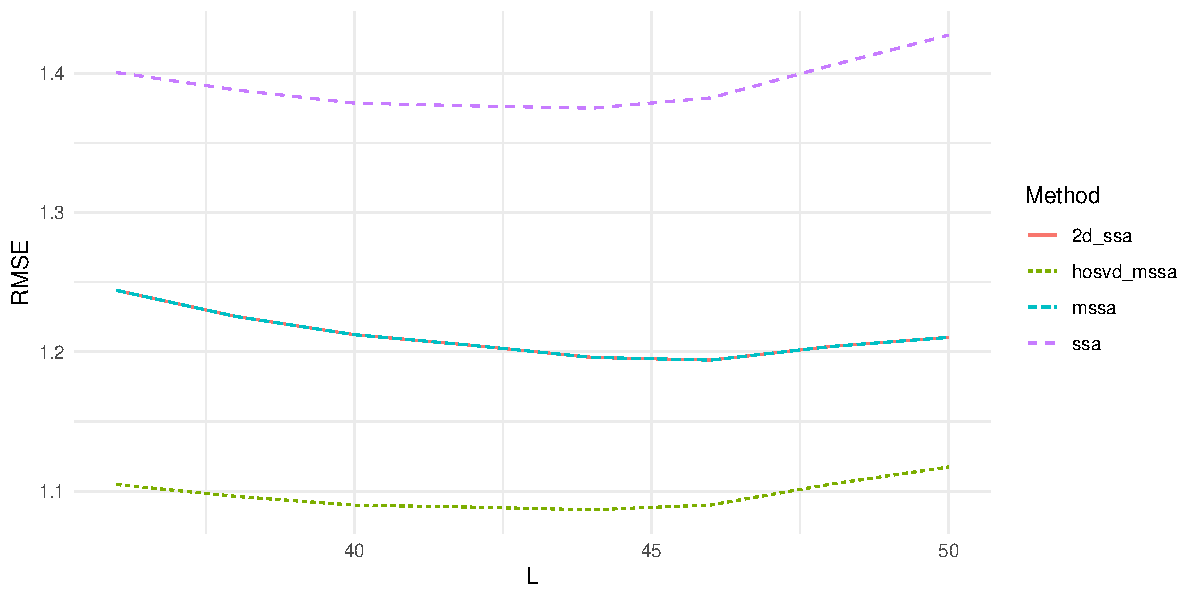
\includegraphics[width=.66\linewidth]{two-series-first}\hfill
            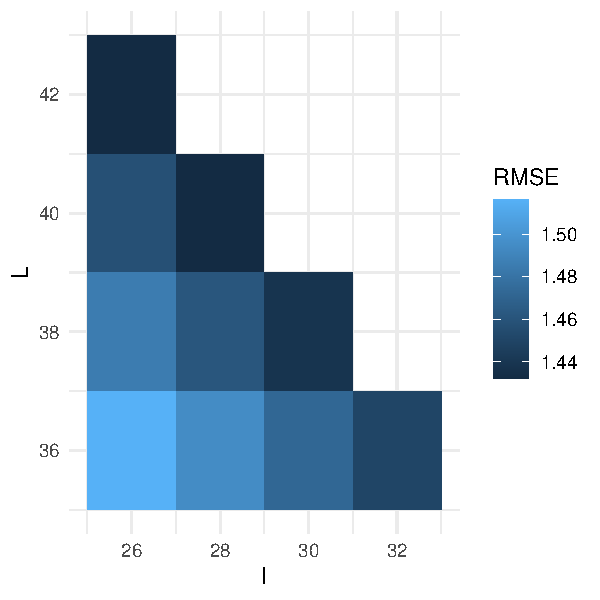
\includegraphics[width=.34\linewidth]{two-series-first_hooi}
            \caption{$\omega_1=\omega_2=1/12$, $\psi_1=\psi_2=0$}
        \end{subfigure} \par\medskip
        \begin{subfigure}{\linewidth}
            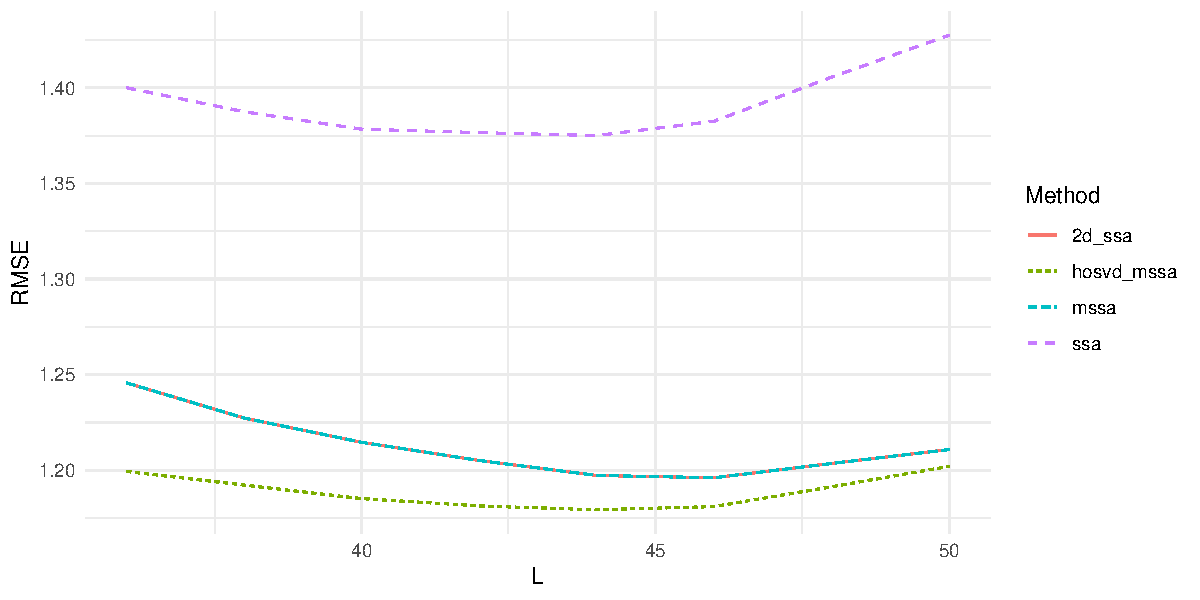
\includegraphics[width=.66\linewidth]{two-series-second}\hfill
            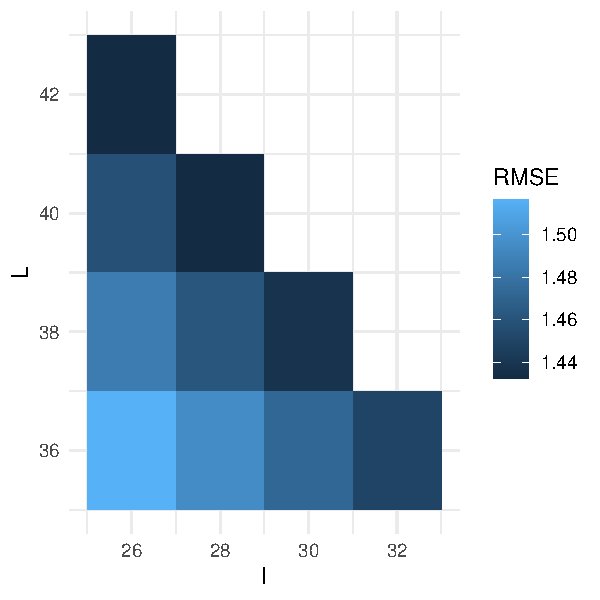
\includegraphics[width=.34\linewidth]{two-series-second_hooi}
            \caption{$\omega_1=\omega_2=1/12$, $\psi_1=0$, $\psi_2=\pi / 4$}
        \end{subfigure}
        \begin{subfigure}{\linewidth}
            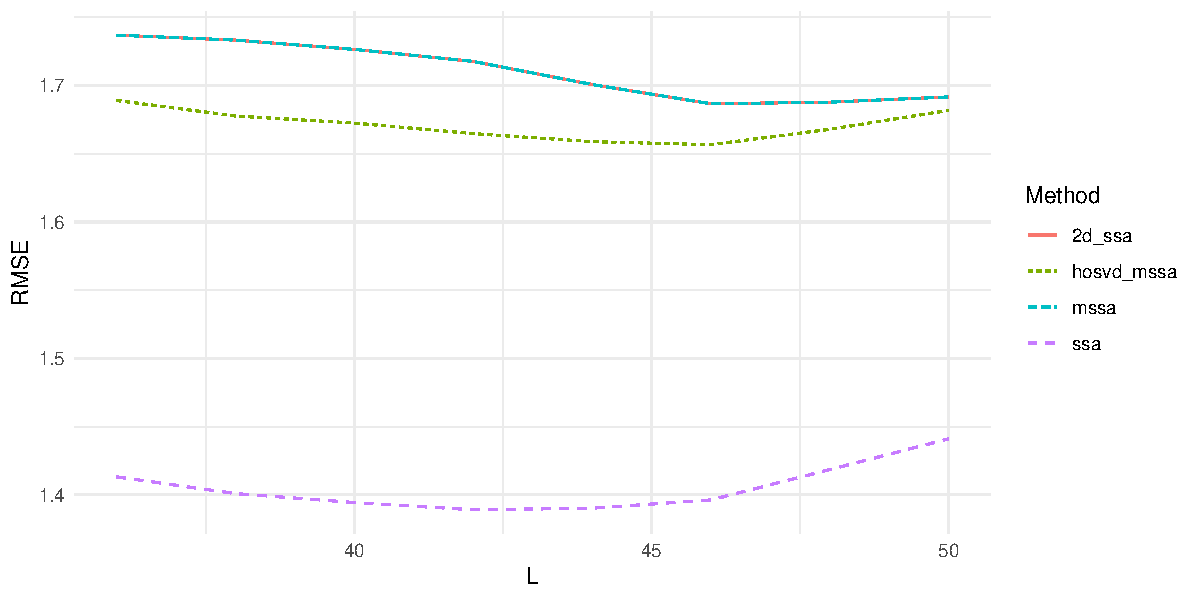
\includegraphics[width=.66\linewidth]{two-series-third}\hfill
            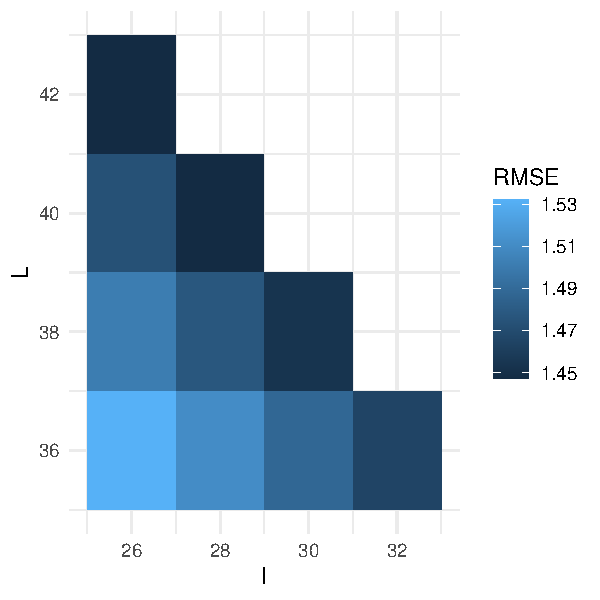
\includegraphics[width=.34\linewidth]{two-series-third_hooi}
            \caption{$\omega_1=1/12$, $\omega_2=1/8$, $\psi_1=0$, $\psi_2=\pi / 4$}
        \end{subfigure}
        \caption{Зависимости точности выделения сигнала от длин окна для каждого из методов
        SSA, MSSA, HOSVD-MSSA, 2D-SSA (слева), HOOI-SSA (справа), $P=2$, $a_1=30$, $a_2 = 20$.}
        \label{fig:two-series-example}
    \end{figure}
    \begin{table}[!h]
        \centering
        \caption{Сравнение SSA, HOOI-SSA, MSSA, HOSVD-MSSA и 2D-SSA: ранги сигнала
        вида~\eqref{eq:general-signal-example}, $P=5$.}
        \begin{tabular}{c|cccc}
            Параметры     & (HOOI) SSA & (HOSVD) MSSA & $r_3$ & 2D-SSA \\
            \hline
            \begin{tabular}{c}
                $a_p=30$     \\
                $\omega_p = \frac 1 {12}$,
                $\psi_p = 0$ \\
            \end{tabular} & 2          & 2            & 1     & 2      \\
            \hline
            \begin{tabular}{c}
                $a_1 = a_4 = 30$ \\
                $a_2 = a_5 =20$,
                $a_3=25$         \\
                $\omega_p = \frac 1 {12}$,
                $\psi_p = 0$     \\
            \end{tabular} & 2          & 2            & 1     & 6      \\
            \hline
            \begin{tabular}{c}
                $a_p=30$,
                $\omega_p = \frac 1 {12}$, \\
                $\psi_p = 2(p-1)\pi / 3$
            \end{tabular} & 2          & 2            & 2     & 2      \\
            \hline
            \begin{tabular}{c}
                $a_p=30$,
                $\psi_p = 2(p-1)\pi / 3$                        \\
                $\omega_1 = \omega_2 = \omega_3 = \frac 1 {12}$ \\
                $\omega_4=\omega_5=\frac 1 8$
            \end{tabular} & 2          & 4            & 4     & 10     \\
            \hline
        \end{tabular}\label{tab:ex-five-series-ranks}
    \end{table}
    \begin{table}[!h]
        \centering
        \caption{Сравнение SSA, HOOI-SSA, MSSA, HOSVD-MSSA и 2D-SSA: минимальные RMSE
        оценки сигнала вида~\eqref{eq:general-signal-example}, $P=5$.}
        \begin{tabular}{c|ccccc}
            \hline
            Параметры     & SSA           & HOOI-SSA & MSSA & HOSVD-MSSA    & 2D-SSA        \\
            \hline
            \begin{tabular}{c}
                $a_p = 30$   \\
                $\omega_p = \frac 1 {12}$,
                $\psi_p = 0$ \\
            \end{tabular} & 1.34          & 1.40     & 0.95 & 0.75          & \textbf{0.73} \\
            \hline
            \begin{tabular}{c}
                $a_1 = a_4 = 30$ \\
                $a_2 = a_5 =20$,
                $a_3=25$         \\
                $\omega_p = \frac 1 {12}$,
                $\psi_p = 0$     \\
            \end{tabular} & 1.38          & 1.41     & 1.07 & \textbf{0.86} & 1.45          \\  \\
            \hline
            \begin{tabular}{c}
                $a_p=30$,
                $\omega_p = \frac 1 {12}$ \\
                $\psi_p = 2(p-1)\pi / 3$
            \end{tabular} & 1.38 & 1.41 & 1.07 & 1.05 & \textbf{0.84} \\
            \hline
            \begin{tabular}{c}
                $a_p=30$,
                $\psi_p = 2(p-1)\pi / 3$                        \\
                $\omega_1 = \omega_2 = \omega_3 = \frac 1 {12}$ \\
                $\omega_4=\omega_5=\frac 1 8$
            \end{tabular} & \textbf{1.38} & 1.41 & 1.50 & 1.49 & 1.78 \\
            \hline
        \end{tabular}\label{tab:comparison-five-series}
    \end{table}
    \begin{figure}[!h]
        \footnotesize
        \centering
        \begin{subfigure}{.836\linewidth}
            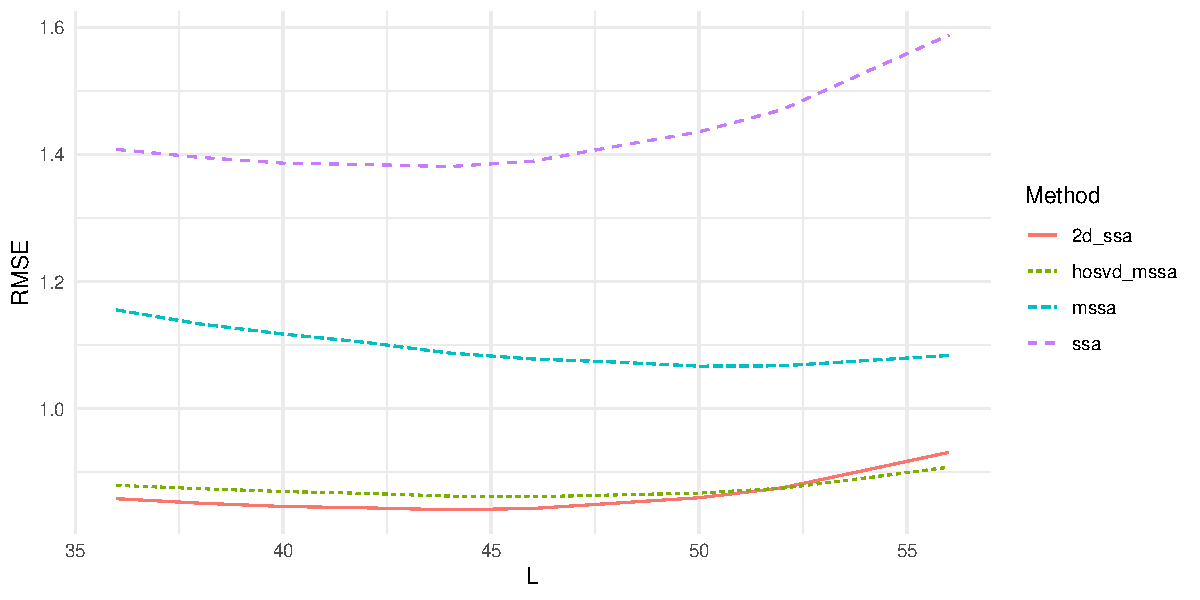
\includegraphics[width=.66\linewidth]{five-series-first}\hfill
            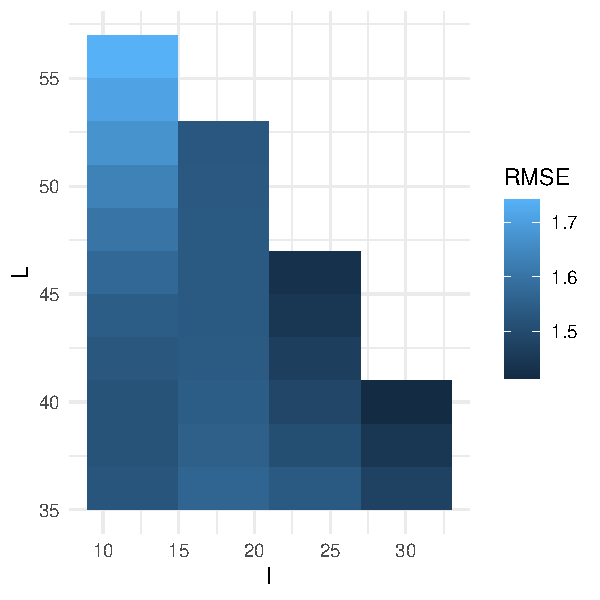
\includegraphics[width=.34\linewidth]{five-series-first_hooi}
            \caption{$a_p = 30$, $\omega_p=1/12$, $\psi_p=0$}
        \end{subfigure} \par\medskip
        \begin{subfigure}{.836\linewidth}
            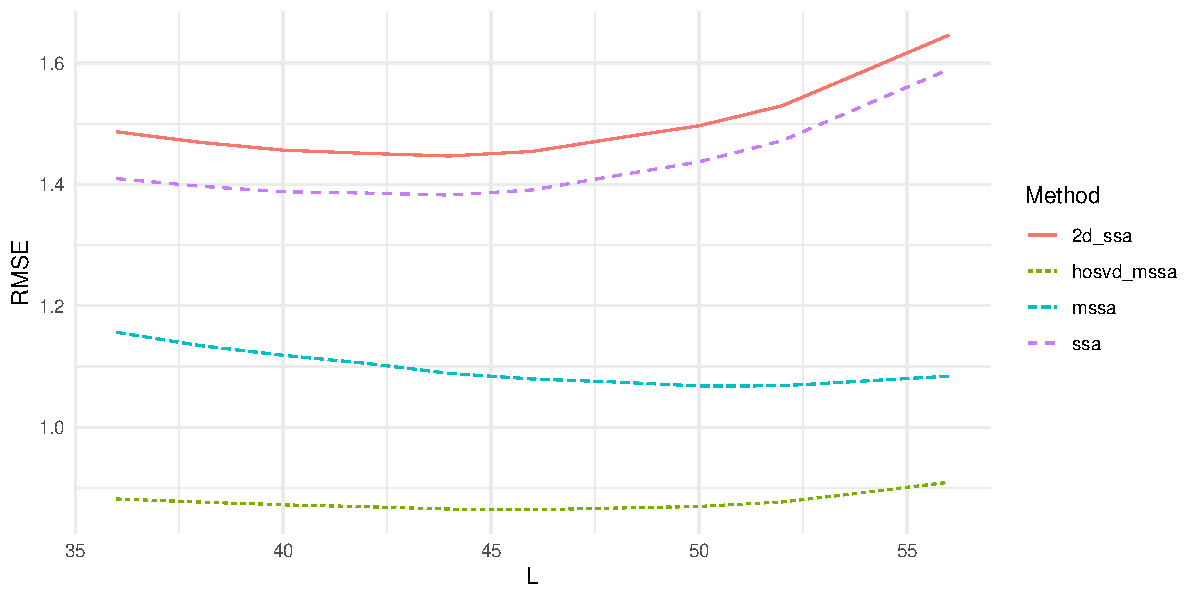
\includegraphics[width=.66\linewidth]{five-series-second}\hfill
            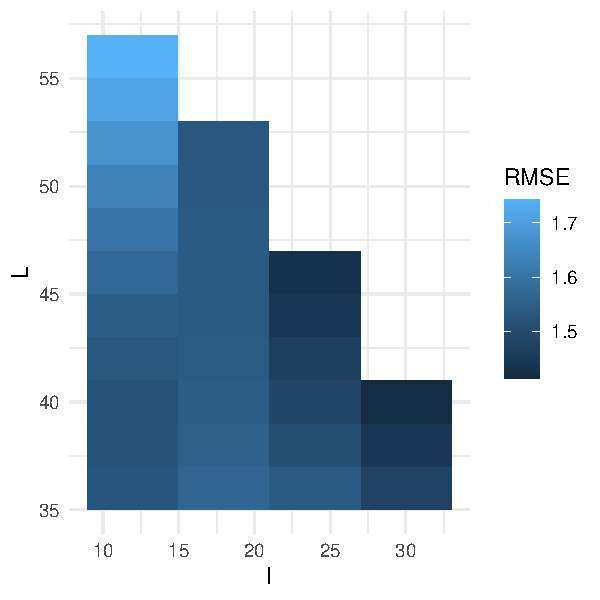
\includegraphics[width=.34\linewidth]{five-series-second_hooi}
            \caption{$a_1=a_4 = 30$, $a_2=a_5=20$, $a_3=25$, $\omega_p=1/12$, $\psi_p=0$}
        \end{subfigure} \par\medskip
        \begin{subfigure}{.836\linewidth}
            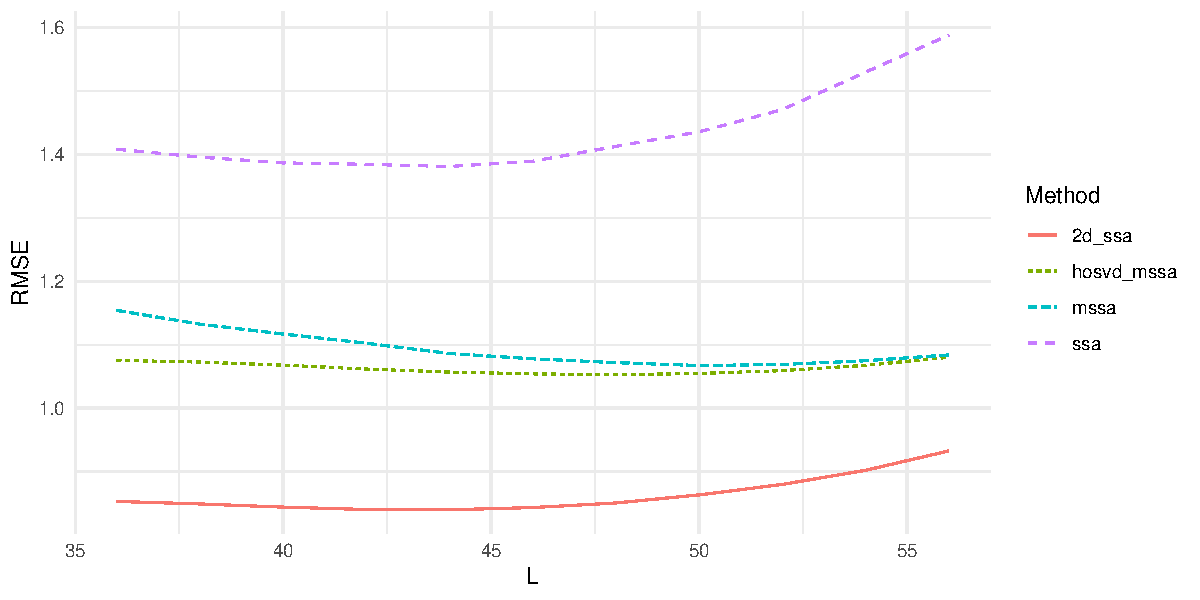
\includegraphics[width=.66\linewidth]{five-series-third}\hfill
            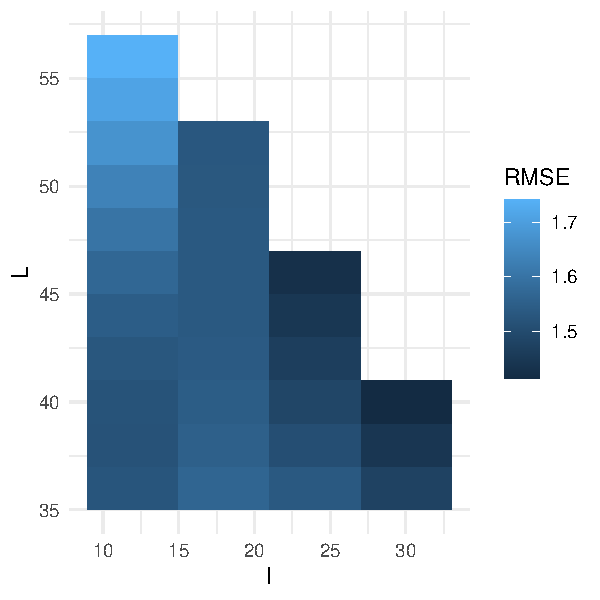
\includegraphics[width=.34\linewidth]{five-series-third_hooi}
            \caption{$a_p = 30$, $\omega_p=1/12$, $\psi_p=2(p-1)\pi/3$}
        \end{subfigure} \par\medskip
        \begin{subfigure}{.836\linewidth}
            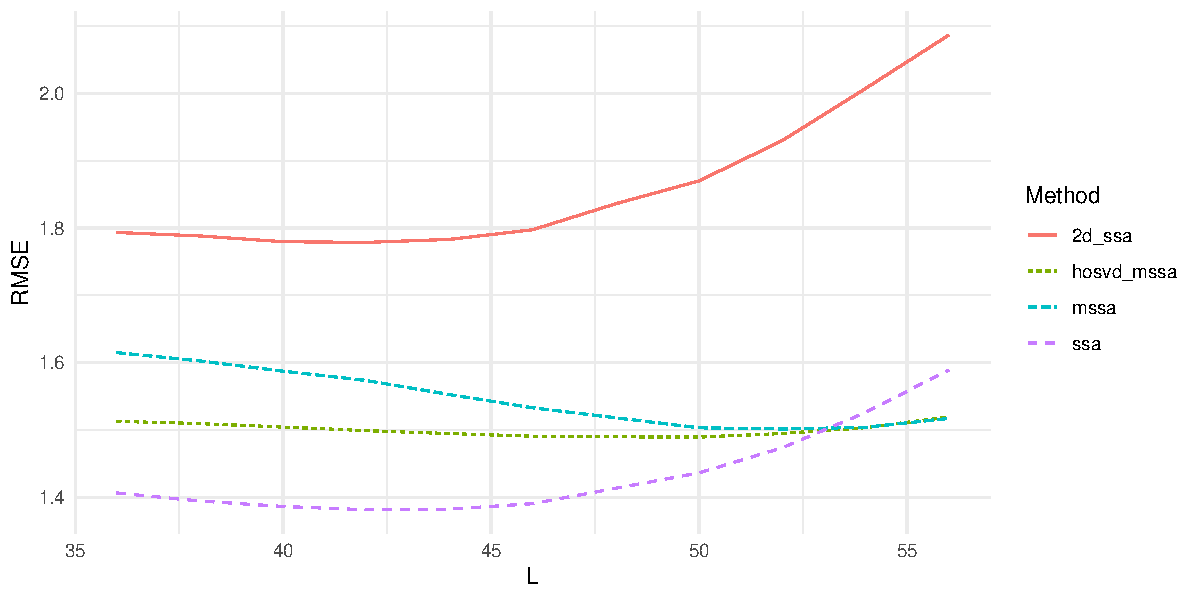
\includegraphics[width=.66\linewidth]{five-series-fourth}\hfill
            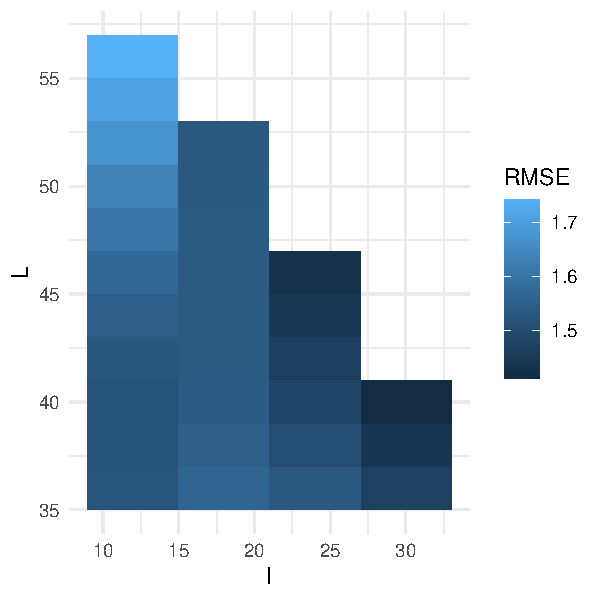
\includegraphics[width=.34\linewidth]{five-series-fourth_hooi}
            \caption{$a_p = 30$, $\omega_1=\omega_2=\omega_3=1/12$, $\omega_4=\omega_5=1/8$, $\psi_p=2(p-1)\pi/3$}
        \end{subfigure}
        \caption{Зависимости точности выделения сигнала от длин окна для каждого из методов
        SSA, MSSA, HOSVD-MSSA, 2D-SSA (слева), HOOI-SSA (справа), $P=5$.}
        \label{fig:five-series-example}
    \end{figure}
    \begin{table}[!h]
        \centering
        \caption{Сравнение SSA, HOOI-SSA, MSSA, HOSVD-MSSA и 2D-SSA: ранги сигнала
        вида~\eqref{eq:general-signal-example}, $P=9$.}
        \begin{tabular}{c|cccc}
            Параметры     & (HOOI) SSA & (HOSVD) MSSA & $r_3$ & 2D-SSA \\
            \hline
            \begin{tabular}{c}
                $a_p=30$     \\
                $\omega_p = \frac 1 {12}$,
                $\psi_p = 0$ \\
            \end{tabular} & 2          & 2            & 1     & 2      \\
            \hline
            \begin{tabular}{c}
                $a_{p} = a_{p+5} = 30 - 2(p-1)$, $1 \leqslant p \leqslant 4$ \\
                $a_5=22$,
                $\omega_p = \frac 1 {12}$,
                $\psi_p = 0$                                                 \\
            \end{tabular} & 2          & 2            & 1     & 10     \\
            \hline
            \begin{tabular}{c}
                $a_p=30$,
                $\omega_p = \frac 1 {12}$, \\
                $\psi_p = 2(p-1)\pi / 5$
            \end{tabular} & 2          & 2            & 2     & 2      \\
            \hline
            \begin{tabular}{c}
                $a_p=30$,
                $\psi_p = 2(p-1)\pi / 5$                               \\
                $\omega_p = \frac 1 {12}$, $1 \leqslant p \leqslant 7$ \\
                $\omega_8=\omega_9=\frac 1 8$
            \end{tabular} & 2          & 4            & 4     & 10     \\
            \hline
        \end{tabular}\label{tab:ex-nine-series-ranks}
    \end{table}
    \begin{figure}[!h]
        \centering
        \begin{subfigure}{.836\linewidth}
            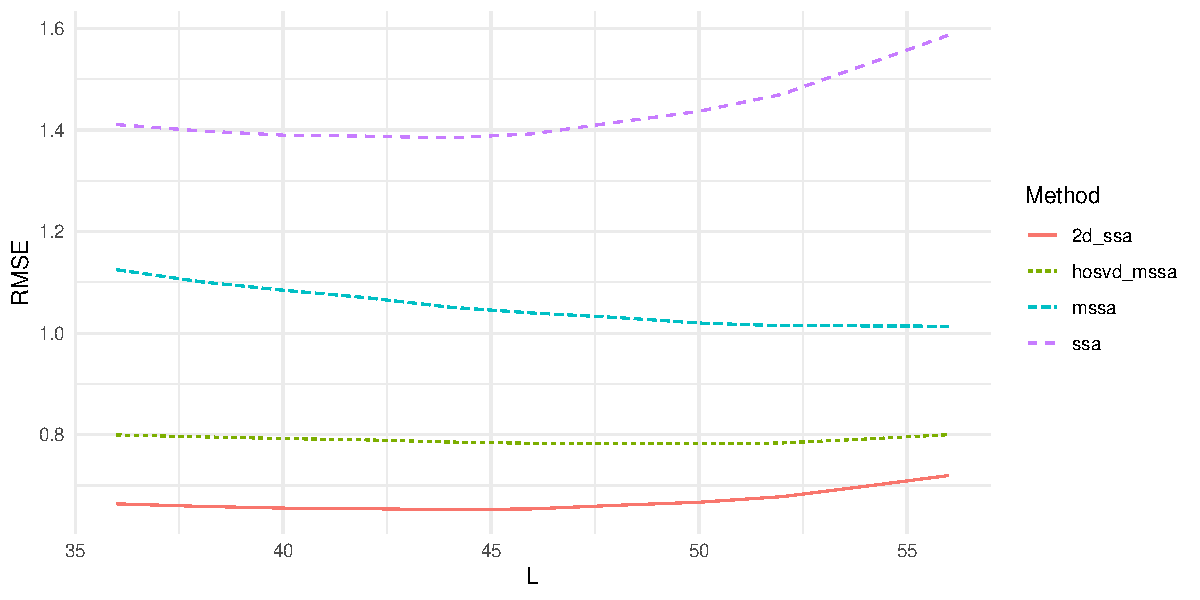
\includegraphics[width=.66\linewidth]{nine-series-first}\hfill
            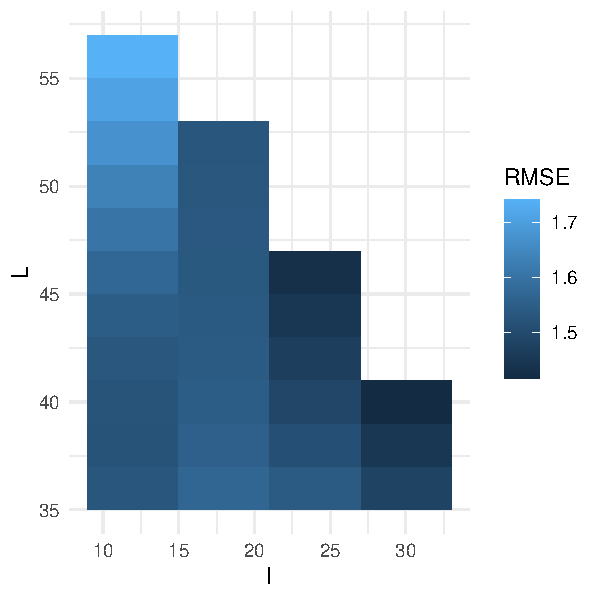
\includegraphics[width=.34\linewidth]{nine-series-first_hooi}
            \caption{$a_p = 30$, $\omega_p=1/12$, $\psi_p=0$}
        \end{subfigure} \par\medskip
        \begin{subfigure}{.836\linewidth}
            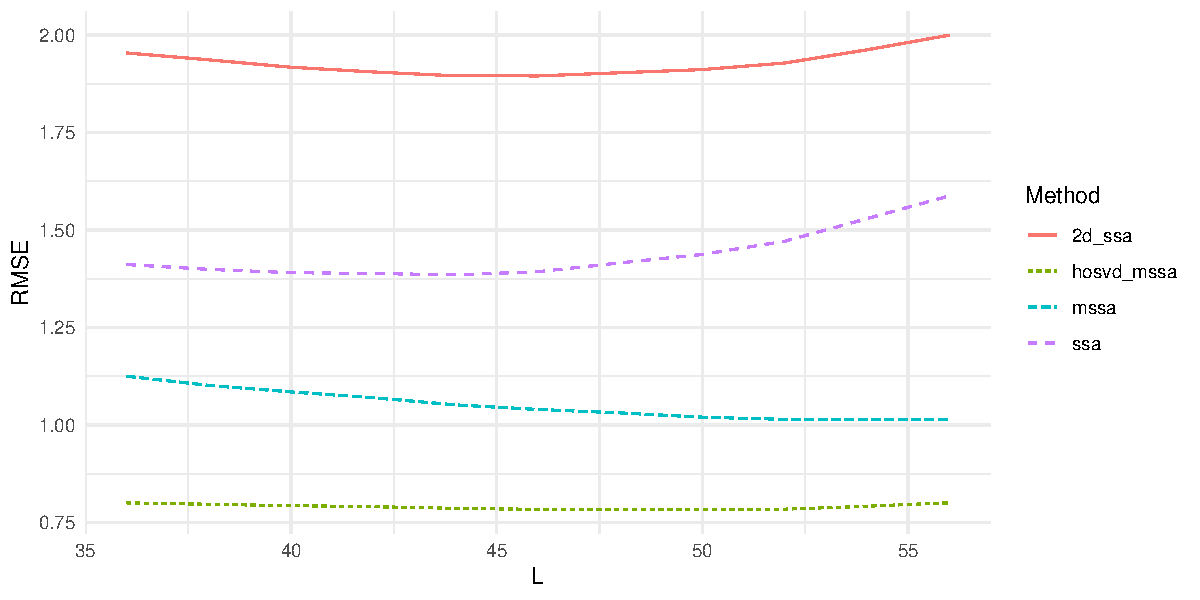
\includegraphics[width=.66\linewidth]{nine-series-second}\hfill
            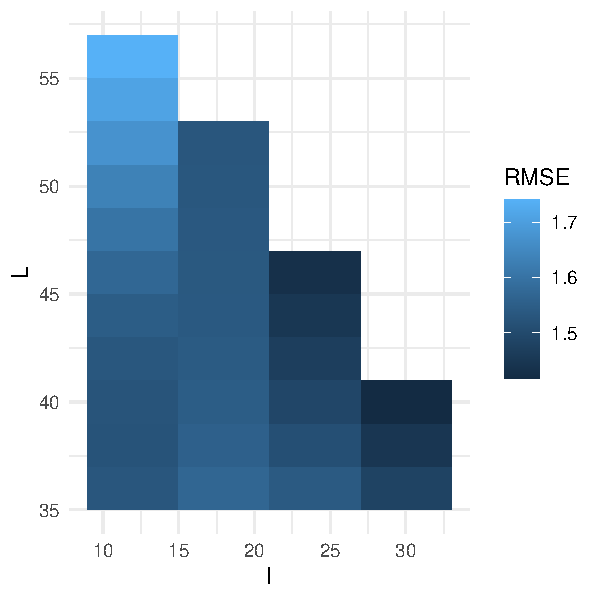
\includegraphics[width=.34\linewidth]{nine-series-second_hooi}
            \caption{$a_{p} = a_{p+5} = 30 - 2(p-1)$, $1 \leqslant p \leqslant 4$,
                $a_5=22$, $\omega_p=1/12$, $\psi_p=0$}
        \end{subfigure} \par\medskip
        \begin{subfigure}{.836\linewidth}
            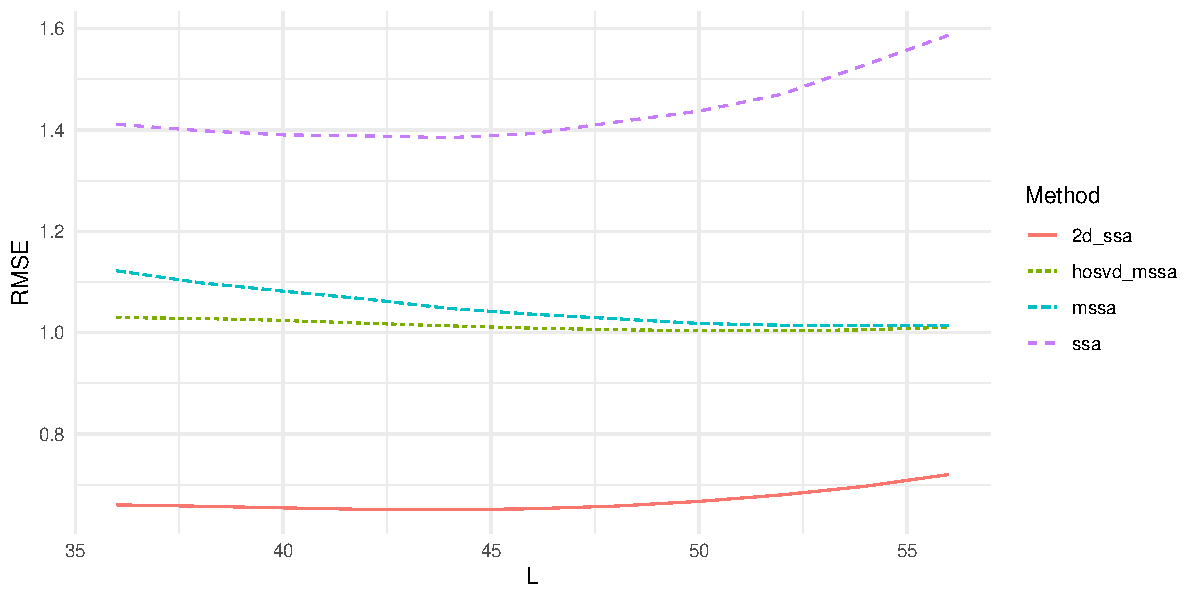
\includegraphics[width=.66\linewidth]{nine-series-third}\hfill
            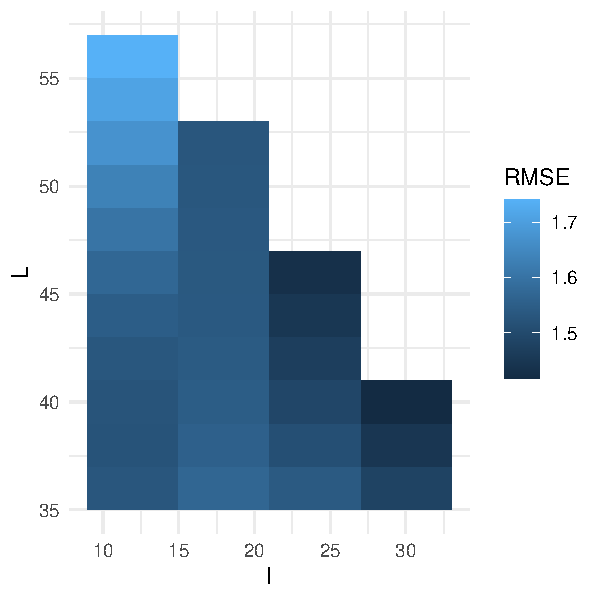
\includegraphics[width=.34\linewidth]{nine-series-third_hooi}
            \caption{$a_p = 30$, $\omega_p=1/12$, $\psi_p=2(p-1)\pi/5$}
        \end{subfigure} \par\medskip
        \begin{subfigure}{.836\linewidth}
            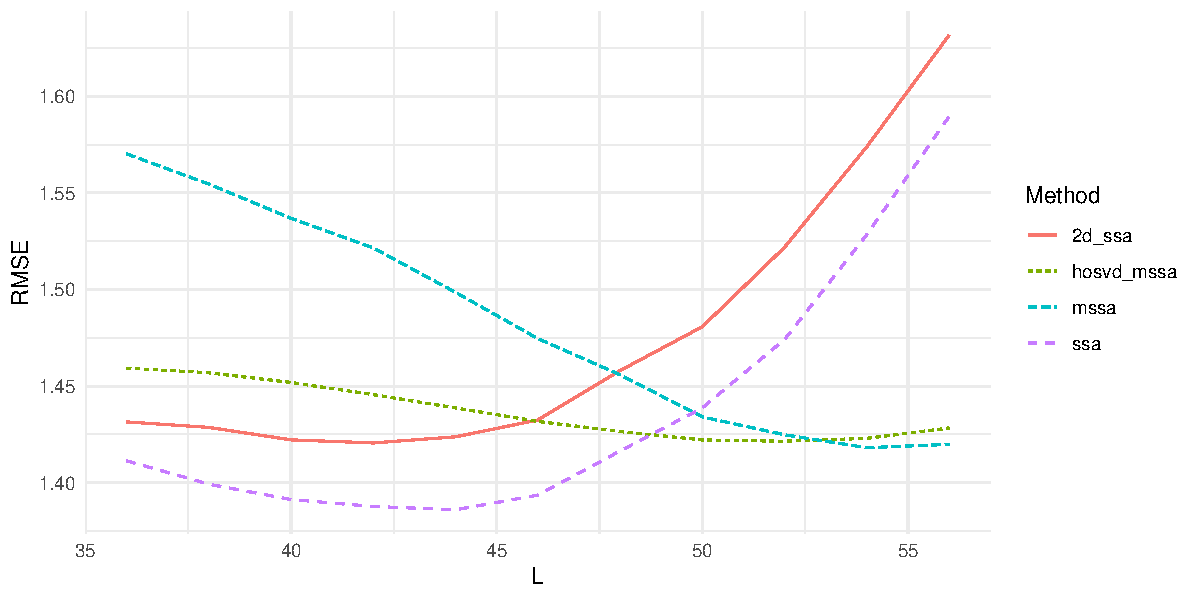
\includegraphics[width=.66\linewidth]{nine-series-fourth}\hfill
            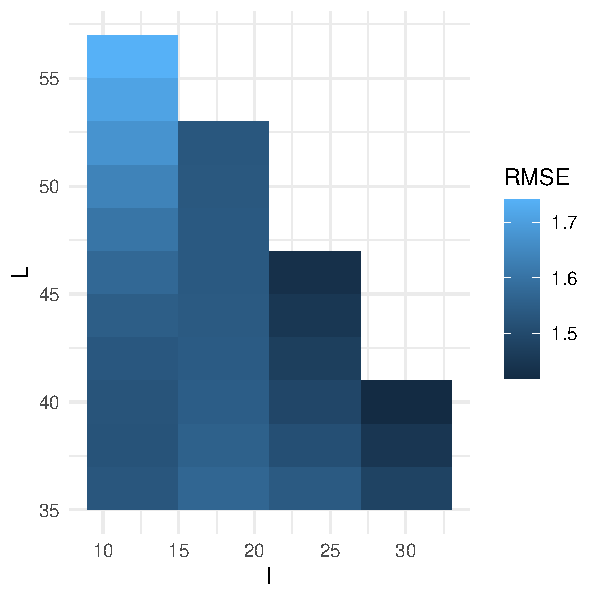
\includegraphics[width=.34\linewidth]{nine-series-fourth_hooi}
            \caption{$a_p = 30$, $\omega_p=1/12$, $1 \leqslant p \leqslant 7$,
                $\omega_8=\omega_9=1/8$, $\psi_p=2(p-1)\pi/5$}
        \end{subfigure}
        \caption{Зависимости точности выделения сигнала от длин окна для каждого из методов
            SSA, MSSA, HOSVD-MSSA, 2D-SSA (слева), HOOI-SSA (справа), $P=9$.}
        \label{fig:nine-series-example}
    \end{figure}

    \FloatBarrier

    \begin{table}[!h]
        \centering
        \caption{Сравнение SSA, HOOI-SSA, MSSA, HOSVD-MSSA и 2D-SSA: минимальные RMSE
        оценки сигнала вида~\eqref{eq:general-signal-example}, $P=9$.}
        \begin{tabular}{c|ccccc}
            \hline
            Параметры     & SSA           & HOOI-SSA & MSSA & HOSVD-MSSA    & 2D-SSA        \\
            \hline
            \begin{tabular}{c}
                $a_p = 30$   \\
                $\omega_p = \frac 1 {12}$,
                $\psi_p = 0$ \\
            \end{tabular} & 1.38          & 1.42     & 1.01 & 0.78          & \textbf{0.65} \\
            \hline
            \begin{tabular}{c}
                $a_{p} = a_{p+5} = 30 - 2(p-1)$ \\
                $1 \leqslant p \leqslant 4$,
                $a_5=22$                        \\
                $\omega_p = \frac 1 {12}$,
                $\psi_p = 0$
            \end{tabular} & 1.38          & 1.42     & 1.01 & \textbf{0.78} & 1.90          \\
            \hline
            \begin{tabular}{c}
                $a_p=30$,
                $\omega_p = \frac 1 {12}$ \\
                $\psi_p = 2(p-1)\pi / 5$
            \end{tabular} & 1.38          & 1.42     & 1.01 & 1.00          & \textbf{0.65} \\
            \hline
            \begin{tabular}{c}
                $a_p=30$,
                $\psi_p = 2(p-1)\pi / 5$                               \\
                $\omega_p = \frac 1 {12}$, $1 \leqslant p \leqslant 7$ \\
                $\omega_8=\omega_9=\frac 1 8$
            \end{tabular} & \textbf{1.39} & 1.42     & 1.42 & 1.42          & 1.42          \\
            \hline
        \end{tabular}\label{tab:comparison-nine-series}
    \end{table}

%    \FloatBarrier


    \section{Численные сравнения в задаче разделения компонент}\label{sec:numerical-comp-sep}
    Рассматриваются временные ряды $\tX = \left(\tX_1: \tX_2: \ldots: \tX_P\right)$,
    $\tX_p = \left(x_1^{(p)}, x_2^{(p)}, \ldots, x_N^{(p)}\right)^{\rmT}$, вида
    \begin{equation*}
        x_n^{(p)} = \hat{s}_n^{(p)} + \tilde{s}_n^{(p)} + \varepsilon_n^{(p)},
    \end{equation*}
    где $\varepsilon_n^{(p)}$ "--- белый гауссовский шум со стандартным отклонением $\sigma = 0.1$.
    Ниже приведены рассматриваемые варианты сигналов $\hat{s}_n^{(p)}$, $\tilde{s}_n^{(p)}$.
    \begin{enumerate}
        \item \textbf{Равные по каналам сигналы:} $N = 44$, $P = 12$,
        \begin{equation}
           \hat{s}_n^{(p)} = 2 \cos(2 \pi n / 5), \quad \tilde{s}_n^{(p)} = \cos(2\pi n /3).
           \label{eq:sep-same}
        \end{equation}
        \item \textbf{Сигналы по каналам отличаются амплитудой:} $N = 44$, $P = 12$,
        \begin{gather}
            \hat{s}_n^{(p)} = 2 c_1^{(p)} \cos(2 \pi n / 5), \quad \tilde{s}_n^{(p)} = c_2^{(p)}\cos(2\pi n /3),
            \label{eq:sep-coeffs}\\
            c_1 = \left(-0.63, 0.18, -0.84, 1.60, 0.33, -0.82, 0.49, 0.74, 0.58, -0.31, 1.51, 0.39\right)\nonumber\\
            c_2 = \left(-0.62, -2.21, 1.12, -0.04, -0.02, 0.94, 0.82, 0.59, 0.92, 0.78, 0.07, -1.99 \right). \nonumber
        \end{gather}
        Амплитуды $c_j^{(p)}$ взяты случайным образом из распределения $\rmN(0, 1)$ и фиксированы для каждой
        реализации шума и для всех дальнейших примеров.
        \item \textbf{Фазы сигналов меняются линейно по номеру канала:} $N = 44$, $P = 12$,
        \begin{equation}
            \hat{s}_n^{(p)} = 2 c_1^{(p)} \cos(2 \pi n / 5 + p \pi / 6),
            \quad \tilde{s}_n^{(p)} = c_2^{(p)}\cos(2\pi n /3 + p \pi / 9).
            \label{eq:sep-lin-phase}
        \end{equation}
        \item \textbf{Произвольные фазы сигналов:} $N = 44$, $P = 12$,
        \begin{gather}
               \hat{s}_n^{(p)} = 2 c_1^{(p)} \cos(2 \pi n / 5 + \varphi_1^{(p)}),
               \quad \tilde{s}_n^{(p)} = c_2^{(p)}\cos(2\pi n /3 + \varphi_2^{(p)}),
               \label{eq:sep-rand-phase}\\
               \varphi_1 = \left(4.60, 3.00, 2.75, 0.44, 1.99, 4.16, 5.74, 2.88, 4.09, 3.01, 0.53, 2.13\right),\nonumber\\
               \varphi_2 = \left(4.35, 5.41, 1.54, 0.62, 3.26, 2.56, 1.84, 2.09, 1.62, 4.81, 5.50, 5.27\right). \nonumber
        \end{gather}
        Фазы $\varphi_j^{(p)}$ взяты случайным образом из распределения $\rmU(0, 2\pi)$ и фиксированы для
        каждой реализации шума.
        \item \textbf{Разделимость константы от гармоники:} $N = 44$, $P = 12$,
        \begin{equation}
            \hat{s}_n^{(p)} = 3 c_1^{(p)},
            \quad \tilde{s}_n^{(p)} = c_2^{(p)}\cos(2\pi n /3).
            \label{eq:sep-const-cos}
        \end{equation}
        \item \textbf{Разные по каналам частоты:} $N = 59$, $P = 12$,
        \begin{gather}
            \hat{s}_n^{(p)} = 2 \cos(2 \pi n / 5), \quad
            \tilde{s}_n^{(p)} = \begin{cases}
                \cos(2\pi n /3), & 1 \leqslant p \leqslant 10,\\
                0.4 \cos(2 \pi n / 6), & 11 \leqslant p \leqslant 12.
            \end{cases}
            \label{eq:sep-periods}
        \end{gather}
        \item \textbf{Ортогональность пространств третьих направлений траекторных тензоров:} $N = 29$, $P = 12$,
        \begin{gather}
            \hat{s}_n^{(p)} = 2 \cos(2 \pi n / 5) \cos(2 \pi p / 3), \quad
            \tilde{s}_n^{(p)} = 0.5 \cos(2\pi n /3) \cos(2 \pi p / 6).
            \label{eq:sep-orthogonal-3}
        \end{gather}
    \end{enumerate}

    Сравнивались методы MSSA, HOSVD-MSSA и 2D-SSA по точности разделения компонент сигнала.
    В качестве оценки точности разделения компонент сигнала было взято RMSE
    каждой восстановленной компоненты сигнала от истинного её значения по 1000 реализациям шума,
    причём сравнения разных методов производилось на одних реализациях шума при выборе оптимальных
    для каждого метода параметров длины окна $L$.
    Оптимальность длины окна проверялась эмпирически.


    \paragraph{Принцип соотношения компонент сингулярного разложения с компонентами сигнала}
    \label{par:example-components-sep}
    Решение о том, к какой компоненте сигнала относить то или иное слагаемое сингулярного разложения
    траекторной матрицы или тензора, принимается из вида сингулярных векторов, образующих это слагаемое.
    А именно: сингулярный вектор должен иметь такой же вид, как и компонента сигнала.
    Например, если сигнал является суммой двух гармоник с периодами 5 и 3, то в случае MSSA и 2D-SSA
    к первой компоненте имеет смысл относить те слагаемые, левые сингулярные векторы которых являются гармониками
    с периодом 5, а ко второй "--- с периодом 3.
    В случае HOSVD-MSSA к первой компоненте имеет смысл относить те слагаемые, сингулярные векторы по первому и
    второму направлению которых являются гармониками с периодом 5, а ко второй "--- с периодом 3.


    \subsection{Результаты численных сравнений}\label{subsec:numerical-comp-sep}
    В таблице~\ref{tab:comparison-sep-comp} представлены индексы сингулярных векторов, относимых
    к компонентам сигнала: в каждой строке индексы над горизонтальной чертой отвечают компоненте $\hat{s}_n^{(p)}$,
    под горизонтальной чертой "--- компоненте $\tilde{s}_n^{(p)}$.
    В столбце $\gP_i$ выписаны соответствующие множества из алгоритма~\ref{alg:hosvd-mssa-sep},
    принцип их выбора указан в следствии к теореме~\ref{state:hosvd-mssa-sep-condition}.
    \begin{remark}
        Максимальные значения индексов для каждого примера совпадает рангом соответствующего сигнала в терминах
        каждого из методов.
    \end{remark}

    Сигнал $\tilde{s}_n^{(p)}$ в уравнении~\eqref{eq:sep-periods} представляется в виде суммы двух сигналов
    \begin{gather*}
        \tilde{s}_n^{(p)} = \tilde{r}_n^{(p)} + \tilde{q}_n^{(p)},\\
        \tilde{r}_n^{(p)} = \begin{cases}
            \cos(2\pi n /3), & 1 \leqslant p \leqslant 10,\\
            0, & 11 \leqslant p \leqslant 12,
        \end{cases} \\
        \tilde{q}_n^{(p)} = \begin{cases}
            0, & 1 \leqslant p \leqslant 10,\\
            0.4 \cos(2 \pi n / 6), & 11 \leqslant p \leqslant 12,
        \end{cases}
    \end{gather*}
    поэтому считается, что сигнал состоит из трёх компонент: $\hat{s}_n^{(p)}$, $\tilde{r}_n^{(p)}$ и
    $\tilde{r}_n^{(p)}$.
    Из-за этого в таблице~\ref{tab:comparison-sep-comp} в строке, отвечающей сигналу~\eqref{eq:sep-periods} выписаны
    три набора индексов: первый соответствует $\hat{s}_n^{(p)}$, второй "--- $\tilde{r}_n^{(p)}$,
    третий "--- $\tilde{q}_n^{(p)}$.

    По аналогии, в таблице~\ref{tab:comparison-sep-rmse} представлены минимальные значения RMSE восстановленных
    компонент сигналов.
    Жирным шрифтом выделены минимальные по строке значения RMSE для данного сигнала.
    Отличие выделенных значений от остальных в строке значимо при уровне значимости $\alpha=0.05$.

    \paragraph{Выводы из численных сравнений}\label{par:numerical-comparison-sep-res}
    Таким образом, метод HOSVD-MSSA разделяет компоненты сигнала не менее точно, чем метод MSSA во всех
    рассмотренных примерах, причём его точность выше в случае, когда у сигналов не меняются фазы при
    изменении номера сигнала.
    Метод 2D-SSA оказался точнее метода HOSVD-MSSA только в специфическом случае равных амплитуд сигнала,
    что соответствует малому 2D-SSA-рангу такого сигнала.

    \begin{table}[!h]
        \centering
        \caption{Сравнение MSSA, HOSVD-MSSA и 2D-SSA: индексы компонент сигналов.}
        \begin{tabular}{c|ccc}
            Вид сигнала    & (HOSVD) MSSA & $\gP_i$ & 2D-SSA \\
            \hline
            \eqref{eq:sep-same} & \begin{tabular}{c} 1, 2 \\ \hline 3, 4 \end{tabular} &
            \begin{tabular}{c} 1, 2 \\ \hline 1, 2 \end{tabular}    &
            \begin{tabular}{c} 1, 2 \\ \hline 3, 4 \end{tabular}   \\
            \hline
            \eqref{eq:sep-coeffs} & \begin{tabular}{c} 1, 2 \\ \hline 3, 4 \end{tabular} &
            \begin{tabular}{c} 1, 2 \\ \hline 1, 2 \end{tabular}    &
            \begin{tabular}{c} $\overline{1:8}$, 13, 14, 19, 20 \\
                \hline $\overline{9:12}$, $\overline{15:18}$, $\overline{21:24}$  \end{tabular}   \\
            \hline
            \eqref{eq:sep-lin-phase} & \begin{tabular}{c} 1, 2 \\ \hline 3, 4 \end{tabular} &
            \begin{tabular}{c} $\overline{1:4}$ \\ \hline $\overline{1:4}$ \end{tabular}    &
            \begin{tabular}{c} $\overline{1:8}$, 13, 14, 19, 20 \\
                \hline $\overline{9:12}$, $\overline{15:18}$, $\overline{21:24}$  \end{tabular}   \\
            \hline
            \eqref{eq:sep-rand-phase} & \begin{tabular}{c} 1, 2 \\ \hline 3, 4 \end{tabular} &
            \begin{tabular}{c} $\overline{1:4}$ \\ \hline $\overline{1:4}$ \end{tabular}    &
            \begin{tabular}{c} $\overline{1:6}$, $\overline{9:12}$, 17, 18 \\
                \hline 7, 8, $\overline{13:16}$, $\overline{19:24}$ \end{tabular}   \\
            \hline
            \eqref{eq:sep-const-cos} & \begin{tabular}{c} 1 \\ \hline 2, 3 \end{tabular} &
            \begin{tabular}{c} 1, 2 \\ \hline 1, 2 \end{tabular}    &
            \begin{tabular}{c} $\overline{1:5}$, 12 \\ \hline $\overline{6:11}$, $\overline{13:18}$ \end{tabular}   \\
            \hline
            \eqref{eq:sep-periods} & \begin{tabular}{c} 1, 2 \\ \hline 3, 4 \\ \hline 5, 6 \end{tabular} &
            \begin{tabular}{c} $\overline{1:3}$ \\ \hline $\overline{1:3}$ \\ \hline $\overline{1:3}$
            \end{tabular}    &
            \begin{tabular}{c} 1, 2 \\ \hline $\overline{3:6}$, 9, 10 \\
                \hline 7, 8, 11, 12 \end{tabular}   \\
            \hline
            \eqref{eq:sep-orthogonal-3} & \begin{tabular}{c} 1, 2 \\ \hline 3, 4 \end{tabular} &
            \begin{tabular}{c} 1 \\ \hline 2 \end{tabular}    &
            \begin{tabular}{c} $\overline{1:4}$ \\ \hline $\overline{5:8}$ \end{tabular}   \\
            \hline
        \end{tabular}\label{tab:comparison-sep-comp}
    \end{table}
    \begin{table}[!h]
        \centering
        \caption{Сравнение MSSA, HOSVD-MSSA и 2D-SSA: минимальные RMSE оценок компонент сигналов.}
        \begin{tabular}{c|ccc}
            \hline
            Вид сигнала    & MSSA & HOSVD-MSSA    & 2D-SSA \\
            \hline
            \eqref{eq:sep-same} & \begin{tabular}{c} 0.026 \\ \hline 0.025 \end{tabular} &
            \begin{tabular}{c} 0.019 \\ \hline 0.016 \end{tabular}    &
            \begin{tabular}{c} \textbf{0.014} \\ \hline \textbf{0.014} \end{tabular}   \\
            \hline
            \eqref{eq:sep-coeffs} & \begin{tabular}{c} 0.029 \\ \hline 0.029 \end{tabular} &
            \begin{tabular}{c} \textbf{0.019} \\ \hline \textbf{0.019} \end{tabular}    &
            \begin{tabular}{c} 0.086 \\ \hline 0.083 \end{tabular}   \\
            \hline
            \eqref{eq:sep-lin-phase} & \begin{tabular}{c} \textbf{0.026} \\ \hline \textbf{0.025} \end{tabular} &
            \begin{tabular}{c} \textbf{0.025} \\ \hline \textbf{0.025} \end{tabular}    &
            \begin{tabular}{c} 0.117 \\ \hline 0.114 \end{tabular}   \\
            \hline
            \eqref{eq:sep-rand-phase} & \begin{tabular}{c} \textbf{0.026} \\ \hline \textbf{0.025} \end{tabular} &
            \begin{tabular}{c} \textbf{0.025} \\ \hline \textbf{0.025} \end{tabular}    &
            \begin{tabular}{c} 0.034 \\ \hline 0.033 \end{tabular}   \\
            \hline
            \eqref{eq:sep-const-cos} & \begin{tabular}{c} \textbf{0.017} \\ \hline 0.025 \end{tabular} &
            \begin{tabular}{c} \textbf{0.017} \\ \hline \textbf{0.019} \end{tabular}    &
            \begin{tabular}{c} 0.023 \\ \hline 0.033 \end{tabular}   \\
            \hline
            \eqref{eq:sep-periods} & \begin{tabular}{c} 0.024 \\ \hline 0.024 \\ \hline 0.024 \end{tabular} &
            \begin{tabular}{c} 0.018 \\ \hline \textbf{0.018} \\ \hline \textbf{0.014} \end{tabular}    &
            \begin{tabular}{c} \textbf{0.012} \\ \hline 0.031 \\ \hline 0.026 \end{tabular}   \\
            \hline
            \eqref{eq:sep-orthogonal-3} & \begin{tabular}{c} 0.031 \\ \hline 0.030 \end{tabular} &
            \begin{tabular}{c} \textbf{0.023} \\ \hline \textbf{0.022} \end{tabular}    &
            \begin{tabular}{c} 0.025 \\ \hline 0.024 \end{tabular}   \\
            \hline
        \end{tabular}\label{tab:comparison-sep-rmse}
    \end{table}

    \subsection{Смещение и дисперсия в случай отсутствия HOSVD-MSSA-разделимости}
    
    В случае отсутствия шума, при длине окна, когда в MSSA есть очная разделимость, а в HOSVD-MSSA ее нет, очевидно, MSSA будет точнее разделять компоненты, так как у него будет ошибка равна нулю. Если для HOSVD-MSSA не существует длины окна, дающей точную разделимость, то, очевидно, MSSA при оптимальной длине окна будет лучше, чем HOSVD-MSSA при своей оптимальной длине окна. 
    
    Взглянем на соотношение ошибок с точки зрения разложения средне-квадратичного отклонения в сумму дисперсии и квадрата смещения: $\mathrm{MSE} = \mathrm{VAR} + \mathrm{bias}^2$.
    
    Сделаем следующее предположение о поведении слагаемых в зависимости от дисперсии шума $\sigma^2$, подтверждаемое на практике: при не слишком большом уровне шума, пока одна из компонент сигнала не начинает смешиваться с шумом, верны следующие соотношения:
    \begin{equation}
    \label{eq:var_bias}
    \mathrm{VAR} \sim C\sigma^2, \quad \mathrm{bias} \sim \mathrm{const}.
    \end{equation} 
    Покажем, что за счет того, что дисперсия оценки по HOSVD-MSSA меньше дисперсии оценки по MSSA, начиная с некоторого уровня шума, HOSVD-MSSA начинает точнее оценивать компоненты сигнала, даже если в отсутствии шума он был менее точным. Заодно проверим выполнение  \eqref{eq:var_bias}. Заметим, что $\mathrm{bias}$ совпадает с RMSE в отсутствии шума, так как в этом случае дисперсия нулевая.
    
    Рассмотрим случай $P$-мерного временного ряда длины $N$, который имеет вид
    \[
        \tX = \widetilde{\tS} + \widehat{\tS} + \tE,
    \]
    где $\hat{s}_n^{(p)} = C_p$ а
    $\tilde{s}_n^{(p)} = A_p \cos(2\pi \omega_p n + \varphi_p)$,
    $C_p$, $A_p \ne 0$, $\omega_p \in (0, 1/2)$, $\varepsilon_n^{(p)}$ "--- независимые случайные величины
    с распределением $\rmN(0, \sigma^2)$. \footnote{Почему не выписать просто вид ряда уже с заданными параметрами?}
    Пусть $P=2$, $N=40$, $\omega_1=\omega_2=1/20$, $C_1 = 3$, $C_2=-1.5$, $A_1 = 1$, $A_2 = 2$,
    $\varphi_1 = \varphi_2 = 0$.
    Согласно примеру~\ref{ex:no-sep} в этом случае сигналы $\widetilde{\tS}$ и $\widehat{\tS}$ являются
    разделимыми в смысле MSSA при $L=30$, и не являются разделимыми в смысле HOSVD-MSSA.

    Рассмотрим зависимость среднеквадратичного отклонения оценки сигнала каждым из методов от выбора длины окна
    $L$ при различных вариантах шума
    \begin{enumerate}
        \item отсутствие шума: $\sigma_0 = 0$,
        \item малый шум: $\sigma_1 = 0.5$,
        \item большой шум: $\sigma_2 = 1$.
    \end{enumerate}


    \begin{figure}[!h]
        \centering
        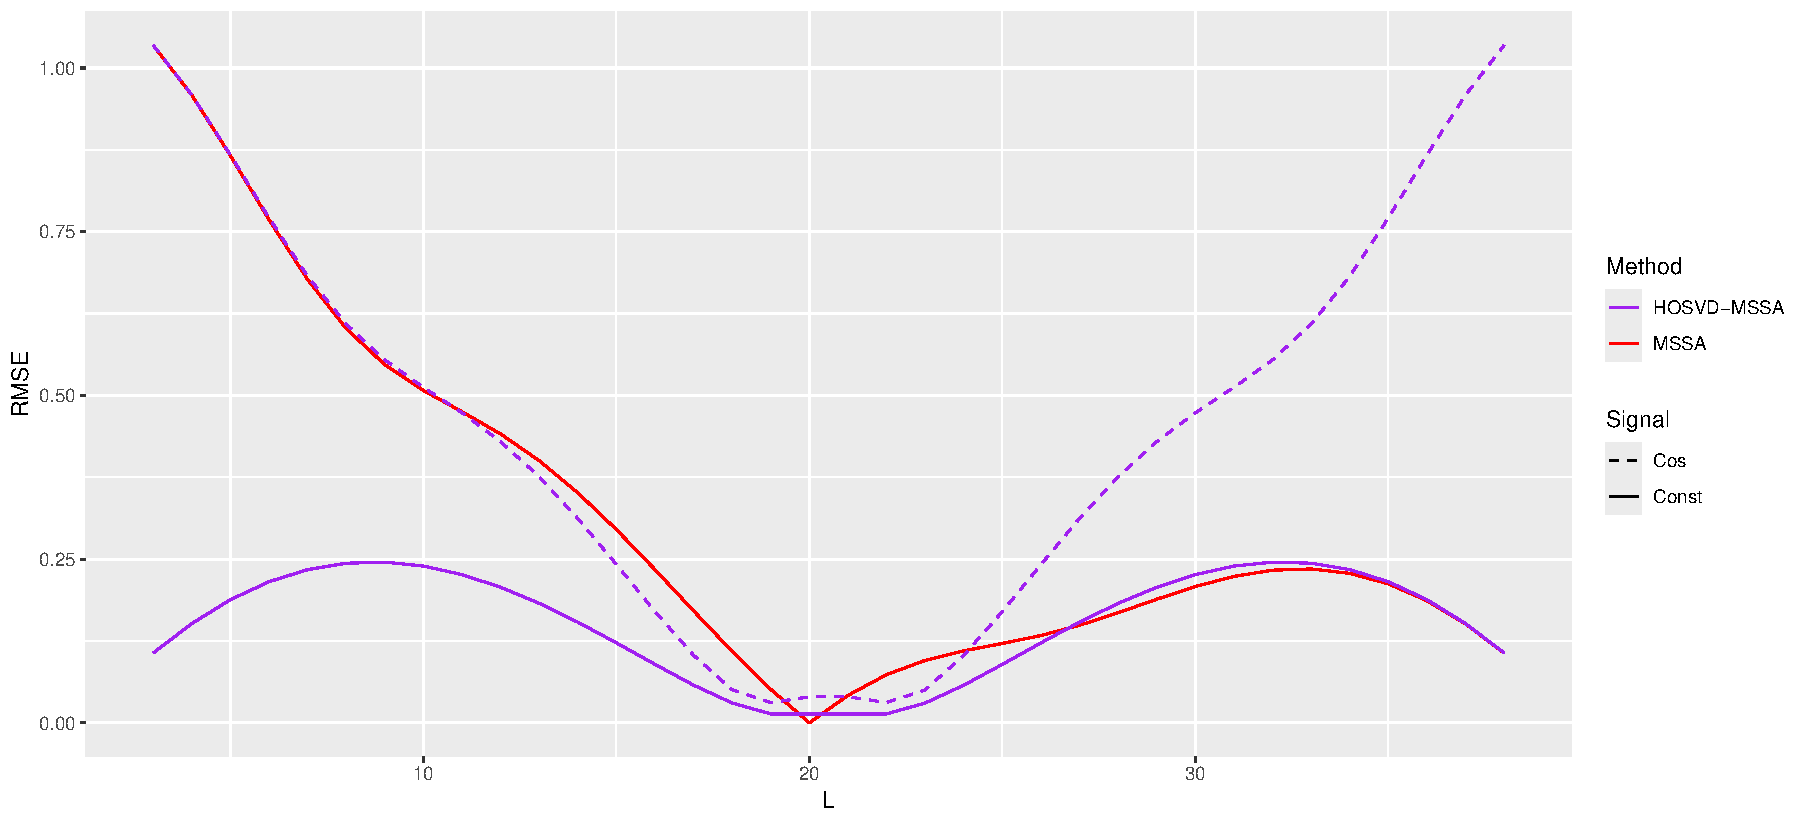
\includegraphics[width=0.87\linewidth]{approx_sep_no_noise}
        \caption{Зависимость RMSE оценки сигнала от длины окна при отсутствующем шуме}
        \label{fig:approx-sep-no-noise}
    \end{figure}
    \begin{figure}[!h]
        \centering
        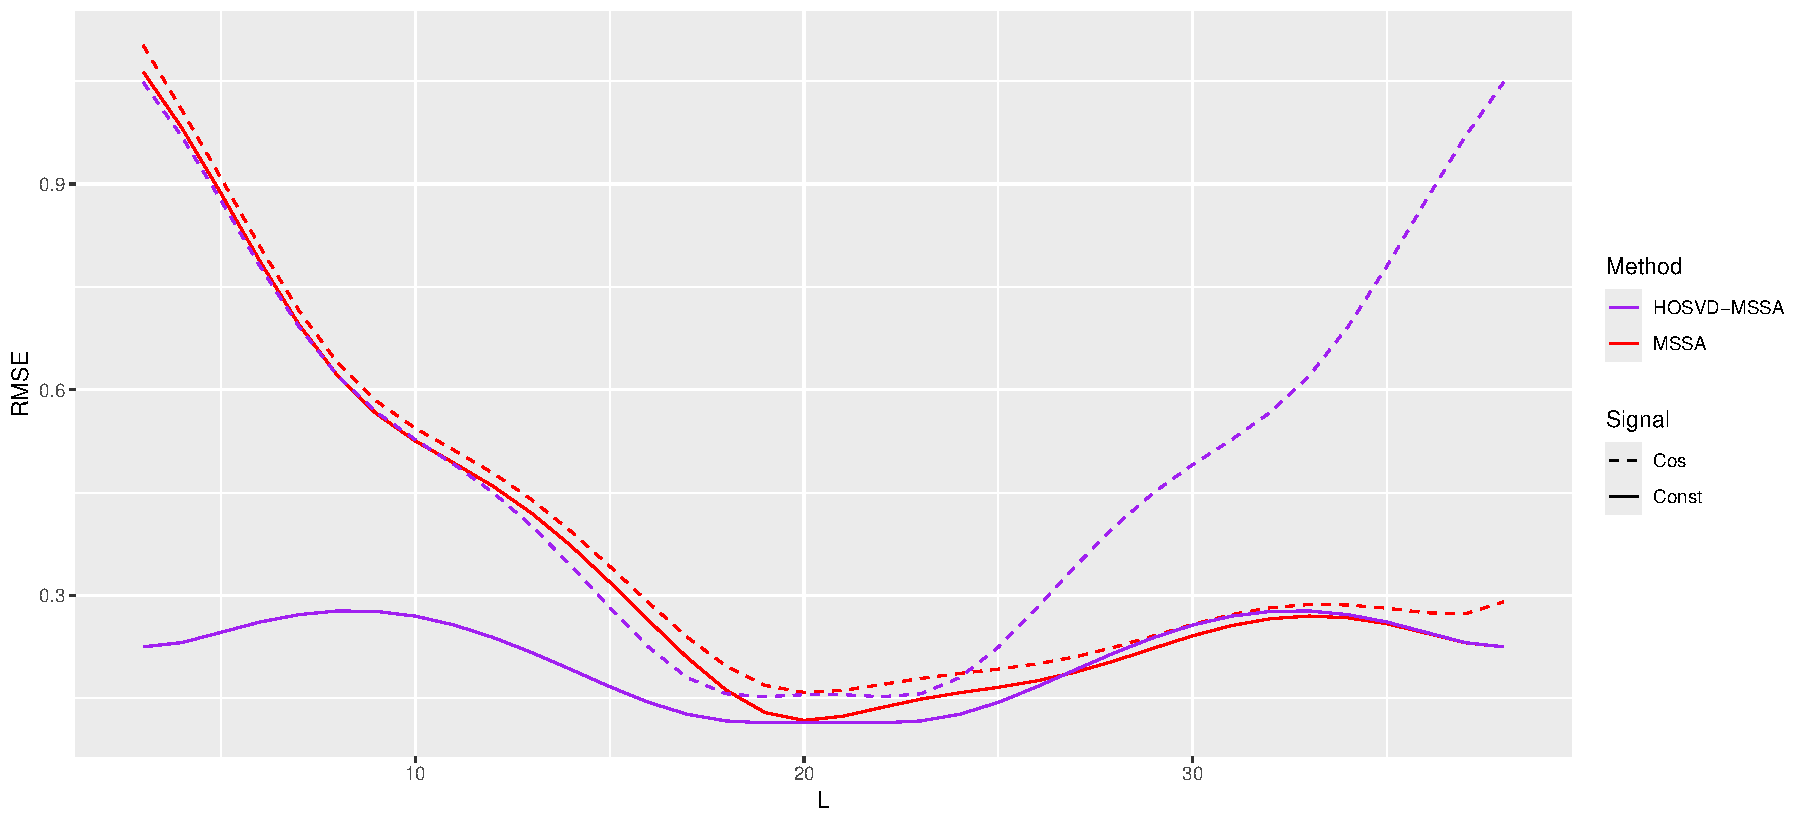
\includegraphics[width=0.87\linewidth]{approx_sep_small_noise}
        \caption{Зависимость RMSE оценки сигнала от длины окна при малом шуме}
        \label{fig:approx-sep-small-noise}
    \end{figure}
    \begin{figure}[!h]
        \centering
        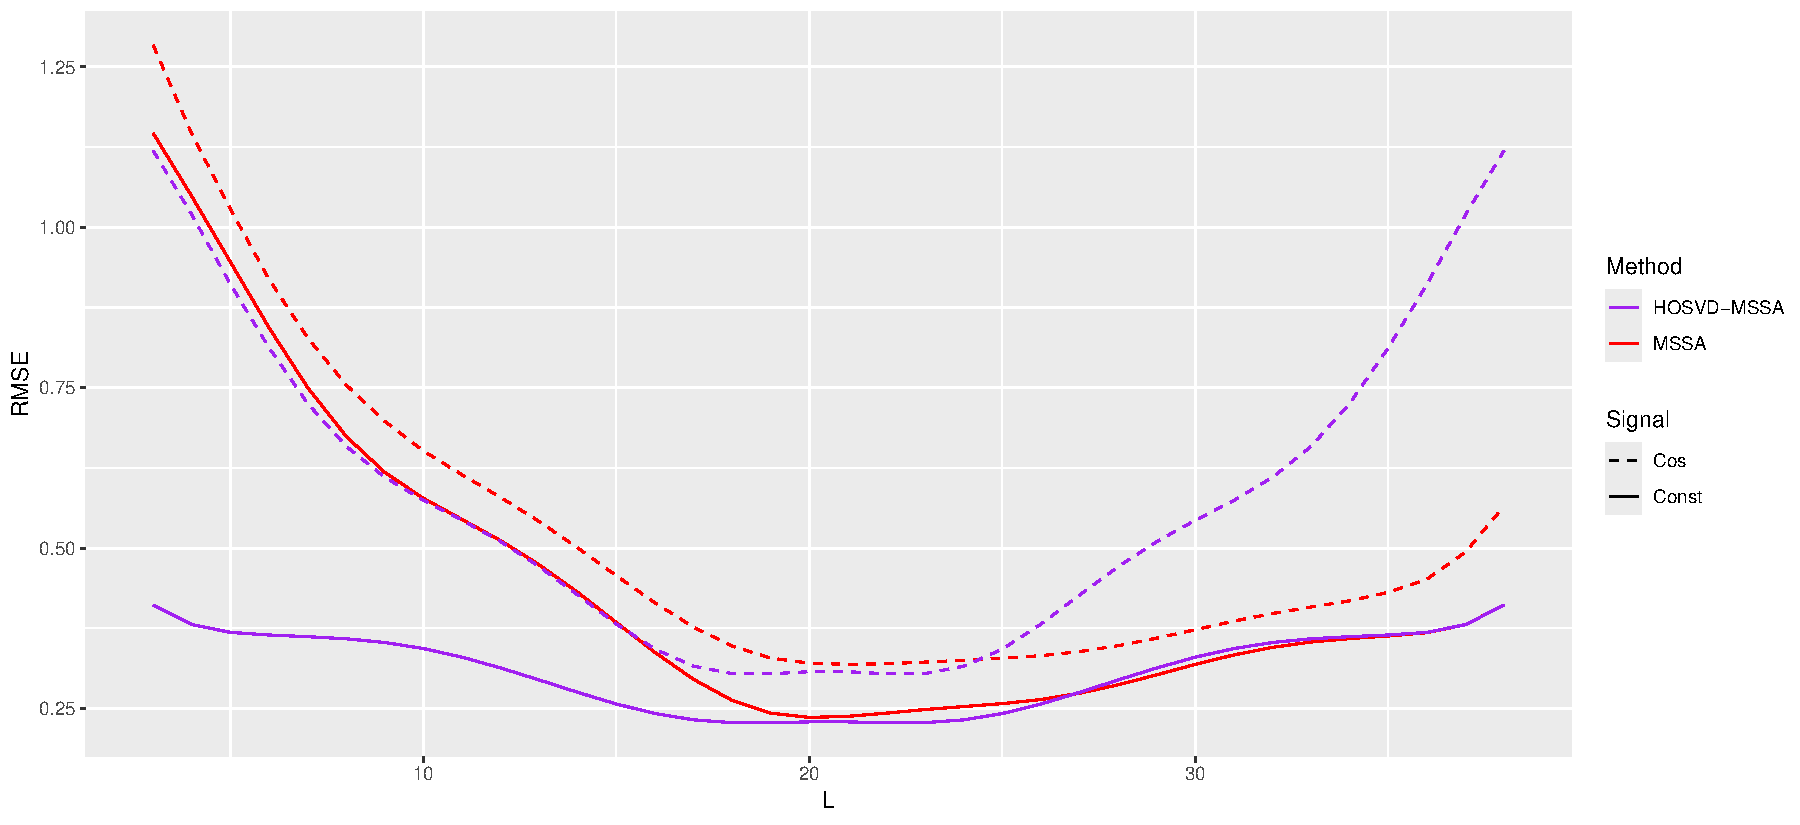
\includegraphics[width=0.87\linewidth]{approx_sep_large_noise}
        \caption{Зависимость RMSE оценки сигнала от длины окна при большом шуме}
        \label{fig:approx-sep-large-noise}
    \end{figure}

    На рисунках~\ref{fig:approx-sep-no-noise},~\ref{fig:approx-sep-small-noise} и~\ref{fig:approx-sep-large-noise}
    изображены графики зависимости RMSE оценок разделённых компонент сигнала для методов MSSA и HOSVD-MSSA от
    параметра длины окна $L$.
    Для каждой длины окна RMSE было посчитано по 500 реализациям шума, причём для различных длин окна
    и для различных методов восстановления при одной длине окна реализации шума совпадали.
    Индексы компонент разложения, относимых к той или иной компоненте сигнала, были взяты равными тем, что
    были описаны в таблице~\ref{tab:comparison-sep-comp} для сигнала~\eqref{eq:sep-const-cos}.

    Из полученных графиков видно, что при отсутствии шума метод MSSA с длиной окна $L=20$ точно разделяет
    компоненты сигнала, а методом HOSVD-MSSA разделить компоненты сигнала без ошибки нельзя ни при какой длине окна,
    что соответствует наличию и отсутствию слабой разделимости для каждого из методов соответственно.
    Значение RMSE в случае отсутствия шума является смещением оценки метода при данном $L$, обозначим
    это смещение $B$.

    При добавлении малого шума преимущество MSSA пропадает, и при большинстве значений параметра $L$ метод
    HOSVD-MSSA разделяет компоненты точнее, чем метод MSSA, однако оптимальные значения RMSE для обоих методов
    довольно близки.
    Значение $\hat{\sigma}_1^2 = \text{RMSE}^2 - B^2$ является оценкой дисперсии оценки компоненты сигнала при
    малом шуме.
    При добавлении большего шума метод HOSVD-MSSA начинает демонстрировать преимущество с точки зрения точности
    разделения компонент сигнала для большинства значений длин окна $L$.

    Увеличение преимущества метода HOSVD-MSSA с увеличением дисперсии шума объясняется тем, что оценки
    компонент сигнала, полученные этим методом, имеют меньшую дисперсию, чем соответствующие оценки, полученные
    методом MSSA, а так как увеличение дисперсии шума соответствующим образом увеличивает и дисперсию оценок
    обоих методов, то дисперсия оценок методом MSSA будет расти быстрее, чем методом HOSVD-MSSA.
    Таким образом, изначальное преимущество MSSA, полученное за счёт меньшего смещения, пропадёт, начиная
    с некоторого значения дисперсии шума.
    
    Чтобы подтвердить верность этих рассуждений, продемонстрируем выполнение предположения~\eqref{eq:var_bias}. Рассмотрим $\hat{\sigma}_2 = \hat{\sigma}_1 \sigma_2 / \sigma_1$
    "--- оценка дисперсии оценки компоненты, соответствующая росту дисперсии шума от $\sigma_1$ к $\sigma_2$.
    Тогда, как показано на графике~\ref{fig:approx-sep-errors}, выполняется приблизительное равенство
    \[
        \sqrt{B^2 + \hat{\sigma}_2^2} \approx \text{RMSE},
    \]
    где RMSE соответствует шуму с $\sigma = 1$.

    \begin{figure}[!h]
        \centering
        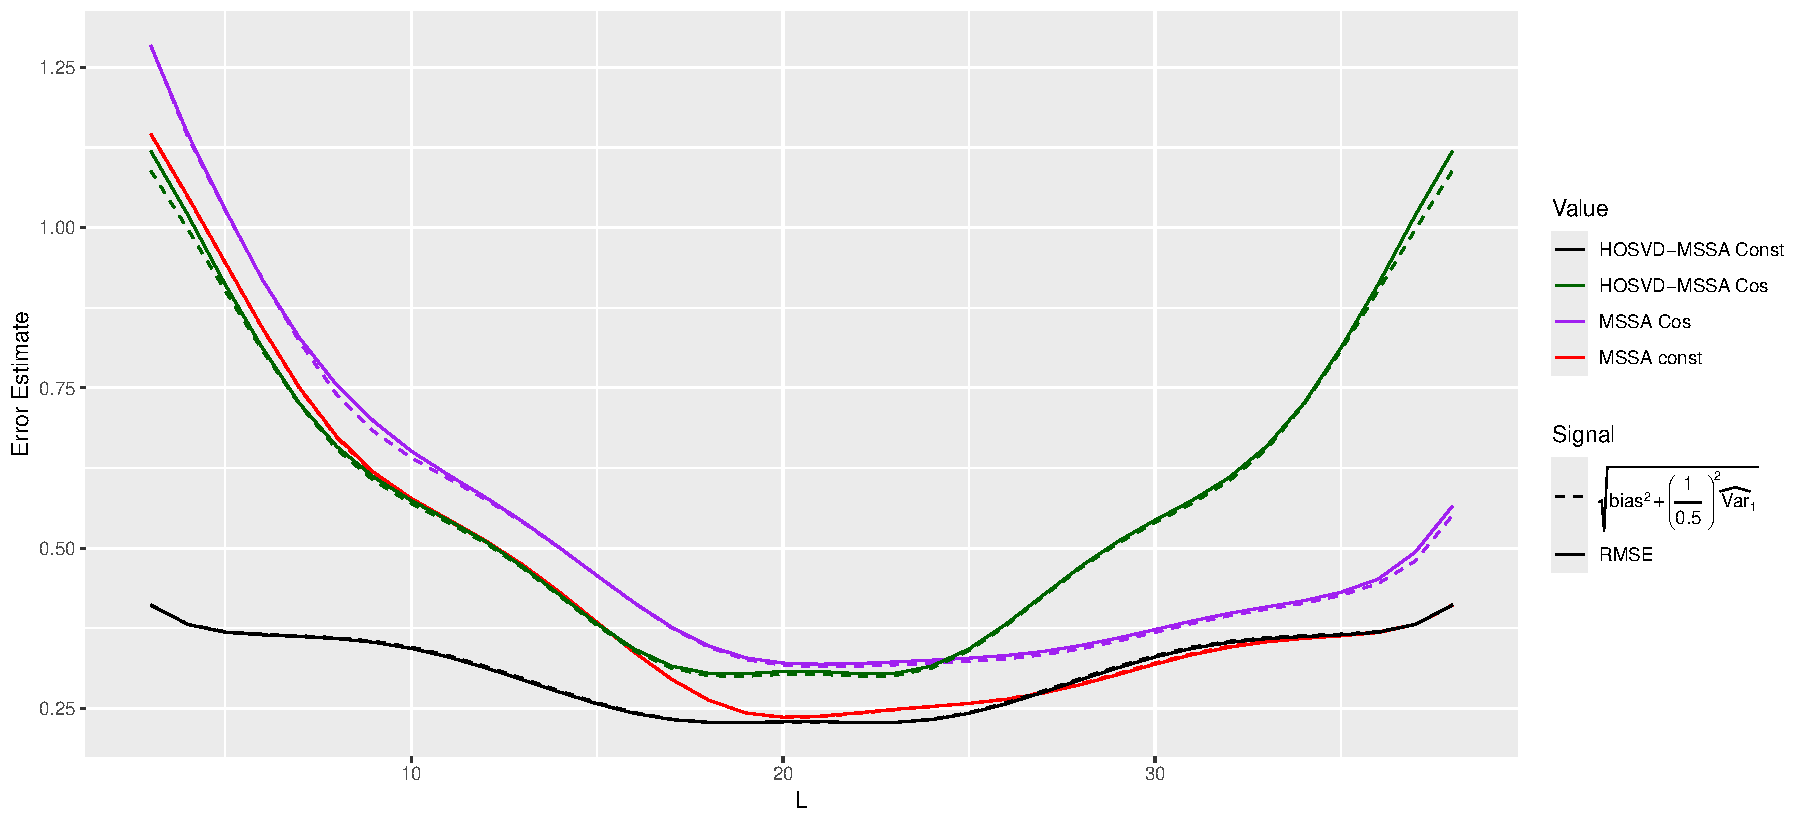
\includegraphics[width=\textwidth]{approx_sep_errors}
        \caption{Сравнение значений RMSE при большой дисперсии шума и аппроксимации $\sqrt{B^2 + \hat{\sigma}_2^2}$ в зависимости от длины окна}
        \label{fig:approx-sep-errors}
    \end{figure}
    
    Таким образом, несмотря на отсутствие слабой разделимости данного сигнала в терминах HOSVD-MSSA,
    тензорная модификация оказывается точнее (хотя и незначительно) базового метода MSSA при достаточно большой дисперсии шума. Пример показывает важность выбора длины окна, соответствующей наилучшей разделимости и уменьшающей смещение.

    \section{Альтернативные тензорные разложения}\label{sec:other-decomp}
    Кроме разложения Таккера, частным случаем которого является HOSVD, существуют и другие тензорные разложения,
    в некотором смысле расширяющие SVD.
    Например, ранговое (каноническое) разложение тензора.
    Суть этого разложения заключается в представлении тензора $\mathcal{A}$ в виде линейной комбинации $R$ тензоров
    ранга $1$, где $R=\operatorname{rank}(\mathcal{A})$.
    Однако нахождение этого ранга в общем случае является NP-трудной задачей~\cite{NP-hard}.

    CP (Canonical Polyadic или CANDECOMP-PARAFAC) approximation~\cite{parafac1, parafac2}"--- итерационный метод
    приближения тензора суммой заданного пользователем числа тензоров ранга $1$.
    То есть по параметру $K$ этот метод вычисляет наилучшее приближение заданного тензора суммой $K$ тензоров ранга $1$.
    Заметим, что из-за отсутствия каких-либо требований к ортогональности в определении рангового разложения тензора,
    многие свойства, верные в теории SSA, могут потерять справедливость при использовании этого разложения.

    Рассмотрим ряды $\tilde{x}_n=3,\, \hat{x}_n=\sin(2\pi n / 3)$, $n \in \overline{0:15}$.
    Построим по этим рядам траекторные тензоры с параметрами $I=L=6$.
    Тогда ранг траекторного тензора $\tilde{\mathcal{X}}$, соответствующего константному ряду, равен $1$, так как его
    можно представить в виде
    \[
        \tilde{\mathcal{X}} = 3 X\circ X \circ X,
    \]
    где $X=(1,\, 1,\, 1,\, 1,\, 1,\, 1)$.
    Ранг траекторного тензора $\hat{\mathcal{X}}$, соответствующего синусу, равен $3$, так как его можно представить в виде
    \[
        \hat{\mathcal{X}}=\sum_{k=1}^{3}\lambda_i X_i \circ Y_i\circ Z_i,
    \]
    где $\lambda_1 \approx 160.56$, $\lambda_2 \approx 65.69$, $\lambda_3 \approx 123.76$,
    \begin{align*}
        \mathbf{X}=[X_1,\, X_2,\, X_3] & \approx
        \begin{pmatrix}
            -0.16 & 0.25  & 0.06  \\
            0.25  & -0.06 & -0.25 \\
            -0.09 & -0.19 & 0.19  \\
            -0.16 & 0.25  & 0.06  \\
            0.25  & -0.06 & -0.25 \\
            -0.09 & -0.19 & 0.19
        \end{pmatrix},\\
        \mathbf{Y}=[Y_1,\, Y_2,\, Y_3] & \approx
        \begin{pmatrix}
            -0.25 & -0.15 & 0.21  \\
            0.18  & -0.10 & -0.25 \\
            0.07  & 0.25  & 0.04  \\
            -0.25 & -0.15 & 0.21  \\
            0.18  & -0.10 & -0.25 \\
            0.07  & 0.25  & 0.04
        \end{pmatrix},\\
        \mathbf{Z}=[Z_1,\, Z_2,\, Z_3] & \approx
        \begin{pmatrix}
            -0.10 & -0.25 & -0.01 \\
            0.25  & 0.12  & -0.24 \\
            -0.15 & 0.13  & 0.25  \\
            -0.10 & -0.25 & -0.01 \\
            0.25  & 0.12  & -0.24 \\
            -0.15 & 0.13  & 0.25
        \end{pmatrix},
    \end{align*}
    притом точных приближений двумя тензорами ранга $1$ нет.
    Траекторный тензор ряда $x_n=\tilde{x}_n+\hat{x}_n$, построенный с параметрами $I=L=6$ представим в виде суммы
    \[
        \mathcal{X}=\sum_{k=1}^{4}\lambda_i X_i \circ Y_i\circ Z_i,
    \]
    где $\lambda_1 \approx 320.17$, $\lambda_2 \approx 120.97$, $\lambda_3 \approx 209.38$, $\lambda_4 \approx 648$,
    \begin{align*}
        \mathbf{X}=[X_1,\, X_2,\, X_3,\, X_4] &=
        \begin{pmatrix}
            -0.25 & -0.25 & 0.25  & -0.17 \\
            0.11  & 0.25  & -0.04 & -0.17 \\
            0.14  & 0.00  & -0.21 & -0.17 \\
            -0.25 & -0.25 & 0.25  & -0.17 \\
            0.11  & 0.25  & -0.04 & -0.17 \\
            0.14  & 0.00  & -0.21 & -0.17
        \end{pmatrix},\\
        \mathbf{Y}=[Y_1,\, Y_2,\, Y_3,\, Y_4] &=
        \begin{pmatrix}
            0.25  & -0.25 & -0.25 & -0.17 \\
            -0.08 & 0.21  & -0.00 & -0.17 \\
            -0.17 & 0.04  & 0.25  & -0.17 \\
            0.25  & -0.25 & -0.25 & -0.17 \\
            -0.08 & 0.21  & -0.00 & -0.17 \\
            -0.17 & 0.04  & 0.25  & -0.17
        \end{pmatrix},\\
        \mathbf{Z}=[Z_1,\, Z_2,\, Z_3,\, Z_4] &=
        \begin{pmatrix}
            -0.00 & -0.14 & -0.08 & 0.17 \\
            -0.25 & -0.11 & 0.25  & 0.17 \\
            0.25  & 0.25  & -0.17 & 0.17 \\
            -0.00 & -0.14 & -0.08 & 0.17 \\
            -0.25 & -0.11 & 0.25  & 0.17 \\
            0.25  & 0.25  & -0.17 & 0.17
        \end{pmatrix},
    \end{align*}
    притом точных приближений суммой трёх тензоров ранга $1$ нет.

    По структуре векторов видно, что четвёртая компонента разложения соответствует константному ряду, а остальные три имеют период равный $3$.
    Таким образом, несмотря на отсутствие ограничений на ортогональность в определении ранговых разложений тензора, наблюдается
    разделимость константного и периодического рядов при наличии условий слабой разделимости в терминах SSA и отсутствия
    шума.
    Однако понятия ранга в терминах SSA и в терминах CP различаются, так как в терминах SSA синус с периодом $3$ имеет ранг $2$, а в
    терминах рангового разложения, как показано выше, такой синус имеет ранг $3$.
    \begin{remark}
        Траекторный тензор, соответствующий синусоидальному ряду, будет иметь ранг 2, если рассматривать его
        над полем $\bbC$, так как синус является суммой комплексных экспонент, а траекторный тензор экспоненциального
        ряда имеет ранг 1.
        Утверждения про зависимость ранга тензора от поля, над которым он рассматривается, можно найти в
        работе~\cite{tensors-bg}.
    \end{remark}

    Другим недостатком CP является то, что это итерационный метод со случайным начальным приближением, в связи
    с чем на одних и тех же данных он может выдавать разные результаты, в том числе может как сойтись, так и нет.

    Возможно можно добиться лучших результатов, используя CP или его модификации, если строить тензор по ряду
    некоторым другим образом и подбирать другие параметры разложения.
    Этот вопрос предлагается изучить в будущих работах.
    \newpage


    \section{Заключение}\label{sec:conclusion}
    В работе было показано, что по своим свойствам HO-SSA и HOSVD-MSSA имеют много общего
    с Basic SSA и MSSA соответственно.
    Однако, есть и особенности, кардинально меняющие свойства методов, которые можно использовать для анализа временных рядов.

    В результате исследования методов HO-SSA и HOSVD-MSSA были сделаны следующие выводы:
    методы можно использовать для выделения сигнала, и, в некоторых случаях, разделения компонент сигнала.
    В большинстве рассмотренных примеров, как HOSVD-SSA, так и HOOI-SSA, оказались хуже,
    чем Basic SSA в точности выделения сигнала.
    Удалось построить только один пример, где тензорная модификация выделяет сигнал точнее, чем Basic SSA.
    В работе~\cite{hosvd-hooi-separation} утверждалось преимущество тензорной модификации алгоритма
    ESPRIT, применяемого для оценки частот параметрического сигнала, над базовым алгоритмом в б\'{о}льшем числе случаев.
    В данной работе показано, что это преимущество отсутствует для тензорной модификации алгоритма SSA, применяемого в задачах выделения сигнала и разделения компонент сигнала.
    Исходный код реализации методов HO-SSA на языке программирования R, а также
    примеры его использования можно найти в~\cite{Rcode}.
    Код написан в стиле существующего пакета Rssa~\cite{Rssa}, реализующего многие методы семейства SSA в R.

    С другой стороны, в рассмотренных случаях, когда сигналы имеют вид вещественных гармоник, метод HOSVD-MSSA оказался
    точнее метода MSSA в задаче выделения сигнала и оказался точнее в задаче разделения компонент сигнала
    при условии наличия слабой HOSVD-MSSA-разделимости, либо при условии наличия у шума большой дисперсии.
    В случаях гармонических сигналов с равными амплитудами данный метод оказался менее точным, чем метод 2D-SSA.

    Таким образом, остались открытыми вопросы: найти семейство сигналов, для которых метод HOSVD-MSSA
    разделяет компоненты точнее, чем метод MSSA, исследовать другие тензорные разложения в задачах выделения сигнала
    и разделения компонент (например в работе~\cite{cpd-separation} предлагается использование модификации метода CPD
    "--- Block-Term Decomposition, в задаче разделения комплексных экспонент), а также
    перенести понятие сильной разделимости из теории MSSA на метод HOSVD-MSSA.

    \bibliography{main}
    \bibliographystyle{ugost2008}

\end{document}
